%%& -job-name=targetfile
\documentclass[
        oneside,      %%coloque  % no in\'icio desta linha para imprimir frente e verso
        english,
%	french,
%	spanish,
        brazil
        ]{configcefetmglpd}


\usepackage[T1]{fontenc}
\usepackage[utf8]{inputenc}		%% Para converter automaticamente acentos como digitados normalmente no teclado. Mude utf8 para latin1 se precisar.

%\usepackage{lmodern} %no caso do modelo Latex, pode-se usar a família de fontes lmodern como aqui indicado, no lugar de Arial e Times New Roman.
\usepackage{times}
\usepackage{lastpage}
\usepackage{indentfirst}
\usepackage{color}
\usepackage{graphicx}
\usepackage{float}
\usepackage{placeins} % fornece \FloatBarrier para conter as figuras na seção
\usepackage{svg}
\usepackage{microtype}
\usepackage{hyperref}
\usepackage{xurl}
\usepackage{pdflscape}
\usepackage[printonlyused]{acronym}
\usepackage{multirow}
\usepackage{etoolbox}
\patchcmd{\folhaaprov}{: \capmystring}{:\\\capmystring}{}{\PackageError{tcc-igor}{Falha ao separar o subtitulo da folha de aprovacao}{Verifique folhaaprov.}}
\patchcmd{\folhaaprov}{\MakeUppercase{ \printatitulo} \IfNonempty}{\MakeUppercase{\printatitulo}\IfNonempty}{}{\PackageError{tcc-igor}{Falha ao ajustar o titulo da folha de aprovacao}{Verifique a definicao de folhaaprov na classe.}}
\usepackage{array} % colunas p{} com alinhamento (>{\raggedright\arraybackslash})

\renewcommand{\appendixname}{APÊNDICE}
\usepackage{listings}
\usepackage{subcaption} % Permite adicionar legendas para subfiguras
% Configuração para exibir código .toml
\lstdefinelanguage{toml}{
    keywords={true, false},
    sensitive=true,
    comment=[l]{\#},
    morecomment=[s]{"""}{"""},
    string=[b]",
}

% Configuração para exibir código TypeScript
\lstdefinelanguage{typescript}{
    keywords={break, case, catch, class, const, continue, debugger, default, delete, do, else, enum, export, extends, false, finally, for, function, if, import, in, instanceof, interface, let, new, null, of, return, super, switch, this, throw, true, try, type, typeof, var, void, while, with, yield, async, await, as, from, namespace, readonly, public, private, protected, static, abstract, declare, implements, package},
    keywordstyle=\color{blue}\bfseries,
    ndkeywords={string, number, boolean, any, unknown, never, Record, Array, Promise, ReactNode},
    ndkeywordstyle=\color{teal}\bfseries,
    identifierstyle=\color{black},
    sensitive=true,
    comment=[l]{//},
    morecomment=[s]{/*}{*/},
    commentstyle=\color{gray}\itshape,
    stringstyle=\color{red},
    string=[b]',
    morestring=[b]",
    morestring=[b]`,
}

\lstset{
    language=toml,
    basicstyle=\ttfamily\small,        % Fonte monoespaçada e menor
    keywordstyle=\color{blue},         % Palavras-chave em azul
    commentstyle=\color{gray},         % Comentários em cinza
    stringstyle=\color{red},           % Strings em vermelho
    breaklines=true,                   % Quebra de linhas automáticas
    frame=single,                      % Adiciona uma moldura ao redor do código
    numbers=left,                      % Adiciona numeração das linhas
    numberstyle=\tiny\color{gray},     % Estilo dos números das linhas
    tabsize=2,                         % Tamanho do tabulação
    showstringspaces=false,            % Não mostra espaços em strings
    float=htbp,                        % Listagem vira float: nunca quebra entre páginas
    floatplacement=htbp                % (exigência da banca: listagem em página única)
}

\usepackage{lipsum}    % gera texto aleatório (remover)
\usepackage{soul}
\usepackage{xcolor}
\usepackage{algorithm}
\usepackage{algorithmic}
\usepackage{amsmath}
\usepackage{amssymb}


%% TikZ para os diagramas elaborados pelos autores (casos de uso e arquitetura).
\usepackage{tikz}
\usetikzlibrary{shapes.geometric,positioning,arrows.meta,fit,backgrounds,calc}

%% Ator UML (boneco palito) desenhado como pic, para uso no diagrama de casos de uso.
\tikzset{
  ator/.pic={
    \draw[thick] (0,0) circle (0.20);
    \draw[thick] (0,-0.20) -- (0,-0.80);
    \draw[thick] (-0.30,-0.40) -- (0.30,-0.40);
    \draw[thick] (0,-0.80) -- (-0.25,-1.25);
    \draw[thick] (0,-0.80) -- (0.25,-1.25);
  },
  uc/.style={ellipse, draw, align=center, inner sep=1.5pt,
             minimum height=0.85cm, font=\scriptsize, fill=white},
  pacote/.style={draw, dashed, rounded corners, inner sep=6pt},
  liga/.style={-, thin, gray!70},
  heranca/.style={-{Triangle[open, length=3mm, width=2.5mm]}, thin},
}

\graphicspath{{Figuras/}} % Diretório onde estão localizadas as figuras

%% Hifenização correta de palavras que o babel quebrava de forma indevida
%% (correções apontadas pelo orientador: divisão silábica).
\hyphenation{
  as-si-mi-la-ção re-pre-sen-ta-ção hie-rár-qui-ca ins-tru-ções
  res-pon-sa-bi-li-da-de so-li-ci-ta-ção a-na-li-sa-das mo-ni-tor
  cor-res-pon-den-tes es-pe-cia-li-za-dos
  re-tar-ge-ta-bi-li-da-de bi-bli-o-grá-fi-ca co-men-tá-rios
  con-sci-en-te es-câ-ne-res es-pe-cia-li-za-dos
}

%% Combate aos "Overfull \hbox" apontados pela banca (texto ultrapassando as
%% margens). \emergencystretch autoriza o TeX a afrouxar o espaçamento numa
%% passada final, em vez de estourar a margem.
\emergencystretch=3em

%% Permite quebra de linha dentro de identificadores longos em \texttt{}
%% (ex.: editor-glass-light, LanguageImage), outra fonte dos estouros.
%% Equivale à opção [htt] do pacote hyphenat, feito à mão para não exigir
%% a instalação de pacote adicional.
\makeatletter
\DeclareRobustCommand\ttfamily{%
  \not@math@alphabet\ttfamily\mathtt
  \fontfamily\ttdefault\selectfont
  \hyphenchar\font=`\-\relax}
\makeatother

%% A classe fixa \cftfigurenumwidth em 24pt dentro de \listfigvariadas
%% (configcefetmglpd.cls, l. 296-303). Essa largura não acomoda rótulos de dois
%% dígitos ("Figura 4.13"), e o excedente empurrava o número da página para fora
%% da margem na Lista de Figuras -- exatamente o ponto apontado pela banca.
%% Redefinido aqui para não alterar o arquivo da classe institucional.
\renewcommand{\listfigvariadas}{%
  \setlength{\cftfigurenumwidth}{32pt}%
  \setlength{\cftfigureindent}{0pt}%
  \begingroup
  \listoffigures*
  \endgroup
}

%% A classe aplica \MakeLowercase ao subtítulo (configcefetmglpd.cls, l. 468),
%% o que rebaixava a sigla IDE para "ide" na capa, na folha de rosto e na folha
%% de aprovação. \NoCaseChange preserva a caixa. O \providecommand é apenas
%% salvaguarda para kernels anteriores a 2022, que não trazem o comando.
\providecommand{\NoCaseChange}[1]{#1}

%% -----------------------------------------------------------------------------

%% Obs.: Alguns acentos foram omitidos.

\titulo{Interpretador Dinâmico para Ensino de Programação} %% O título do trabalho deve ser colocado dentro das chaves {}.
\subtitulo{Uma abordagem interativa com Ambiente de Desenvolvimento Integrado
(\NoCaseChange{IDE}) para personalização e execução de comandos definidos pelo usuário}  %% Acrescentar % no início desta linha se NÃO tiver subtítulo. Se tiver,o subtítulo do trabalho deve ser colocado dentro das chaves {}.

\tituloIngles{Dynamic Interpreter for Programming Education: A Web IDE with Configurable Language Grammar} %% O título do trabalho em inglês deve ser colocado dentro das chaves {} .
% \subtituloIngles{subtitle (se tiver)}  %% Acrescentar % no início desta linha se NÃO tiver subtítulo. Se tiver,o subtítulo em inglês do trabalho deve ser colocado dentro das chaves {}.

\autor{Igor Lamoia Queiroz} %%O nome completo do autor deve ser colocado dentro das chaves {}
\autorVirg{Queiroz, Igor Lamoia} %%Acrescentar o sobrenome do autor, separado por vírgula, antes do restante do nome do autor. Ex.: Silva, José da
\autorSobrenome{Queiroz} %% Apenas o último sobrenome dever ser acrescentado dentro das chaves
\matricula{20193015283} %%Matrícula do aluno autor do trabalho

\local{Leopoldina} %%Não alterar
\mesentrega{02} %%Colocar o mes da entrega dentro das chaves {}, em número. Por exemplo, 1 para janeiro; 2 para fevereiro ...
\data{2026} %%Colocar APENAS o ano da entrega dentro das chaves {}. Por exemplo, 2019.

\orientador[Orientador]{Luís Augusto Mattos Mendes} %%Colocar o nome completo do orientador(a) dentro das chaves {}. Entre os colchetes [], use [Orientador] ou [Orientadora] para identificação
\coorientador[Coorientador]{Eduardo Gabriel Reis Miranda} %%Colocar o nome completo do co-orientador(a) dentro das chaves {}. Entre os colchetes [], use [Orientador] ou [Orientadora] para identificação
\orientadorTitulo{Prof. Me.} %%Colocar a titulação do(a) orientador(a) dentro de chaves {}. Ex: Me., Dr., Dra., etc.
\coorientadorTitulo{Prof. Dsc.} %%Colocar a titulação do(a) co-orientador(a) dentro de chaves {}. Ex: Me., Dr., Dra., etc.
\siglaInstituicaoCoorientador{CEFET-MG} %% Alterar caso o coorientado não seja do CEFET-MG

\instituicao{Centro Federal de Educação Tecnológica de Minas Gerais} %% Não alterar
\siglaInstituicao{CEFET-MG} %% Não alterar

\faculdade{Unidade Leopoldina} %% Não alterar

\programa{Engenharia de Computação} %% Não alterar
\objeto{Trabalho de Conclusão de Curso}  %% Trabalho de Conclusão de Curso - graduação ; Dissertação - mestrado
\natureza{\printaobjeto ~apresentado ao Curso de \printaprograma ~do \printainstituicao, do Campus Leopoldina, como parte do requisito para obtenção do título de Bacharel em Engenharia de Computação.} %% Não alterar

% Data da aprovação
\aprovacaoDia{14} %% Colocar dentro das chaves {} o NÚMERO do dia da Data de aprovação. Ex: 15
\aprovacaoMes{fevereiro} %% Colocar dentro das chaves {} o mês por extenso da Data de aprovação. Ex: janeiro
\aprovacaoAno{2026} %%  Colocar dentro das chaves {} o NÚMERO do ano da Data de aprovação. Ex: 2021

% Dados do Avaliador 1
\avaliadorUm{Matheus Ávila Moreira de Paula} % Nome e sobrenome
\titulacaoAvaliadorUm{Prof. Me.} % Titulação
\siglaInstituicaoAvaliadorUm{CEFET-MG} % Sigla da institução de ensino vinculado

% Dados do Avaliador 2
\avaliadorDois{Gabriella Castro Barbosa Costa} % Nome e sobrenome
\titulacaoAvaliadorDois{Prof. Dsc.} % Titulação
\siglaInstituicaoAvaliadorDois{CEFET-MG} % Sigla da institução de ensino vinculado

% Dados da ficha catalográfica
\NumCatalog{AXXX} % Disponibilizado pela biblioteca.
\CDU{CDU XXX.XX} % Disponibilizado pela biblioteca.

%% Abaixo, prencher com os dados da parte final da ficha catalografica
\finalcatalog{1. Interpretador dinâmico. 2. Ensino de programação. 3. Compiladores. 4. Ambiente de Desenvolvimento Integrado. I. Mendes, Luís Augusto Mattos. II. Miranda, Eduardo Gabriel Reis. III. Interpretador Dinâmico para Ensino de Programação.} % alterar com os dados do trabalho


% Pacotes para referência bibliográfica. Não alterar as linhas abaixo
% \usepackage[round, numbers]{natbib} % Referência númérica (não usado nesse trabalho)
  % \usepackage{natbib} % Referência utilizando o sistema autor-data
%% abnt-etal-list=0 desliga a abreviação por "et al." nas Referências, de modo
%% que todos os autores sejam listados (exigência da banca em LAI et al.,
%% SILVA et al. e SILVEIRA et al.). No corpo do texto o "et al." é mantido.
\usepackage[alf,abnt-emphasize=bf,abnt-etal-list=0]{abntex2cite}

\linespread{1.5}
\begin{document}

%%---------------- Elementos Pré-textuais -----------------------------


%% Capa do Trabalho. (Não alterar)
\printacapa

%% Folha de rosto (Não alterar)
\printafolhaderosto{}

%% O aluno deverá solicitar a ficha na página da Biblioteca de Leopoldina.
%% Ficha catalográfica. AO IMPRIMIR, DEIXAR NO VERSO DA FOLHA DE ROSTO. (Não alterar)
\printacatalog


%% Folha de Aprovação. (Não alterar)
\printafolhaaprov{}


%% Dedicatória. ELEMENTO OPCIONAL. Caso desejar não usar, acrescentar % antes de todas as linhas até \end{dedicatoria}
 % \begin{dedicatoria}
 %  		A dedicatória deve ser escrita com o estilo de texto "Dedicatória" e ficar no final da página. Neste local colocam-se pequenos parágrafos (não muitos) homenageando as pessoas importantes da sua trajetória acadêmica.\\
 %  		Este não é um item obrigatório do TCC conforme NBR 14724 \cite{bib:abnt14724}. Caso opte por não colocar dedicatória, deve-se retirar esta seção.
 % \end{dedicatoria}


%% Agradecimentos. ELEMENTO OPCIONAL. Caso desejar não usar, acrescentar % antes de todas as linhas até \end{agradecimentos}
\begin{agradecimentos}
Agradeço à minha família pelo apoio incondicional, incentivo e paciência ao longo desta jornada. Sem vocês, nada disso seria possível.
Meu sincero agradecimento também ao meu orientador, Luís Augusto Mattos Mendes, e ao meu coorientador, Eduardo Gabriel Reis Miranda, pela orientação, dedicação e ensinamentos valiosos que tornaram este trabalho possível.
A todos que, de alguma forma, contribuíram para esta conquista, meu muito obrigado.

\end{agradecimentos}


%% Epígrafe. ELEMENTO OPCIONAL. Deve conter os dados do autor. A obra usada na epígrafe deve constar nas referências.
% \begin{epigrafemais}
% 	`` a epígrafe não é obrigatória conforme a NBR 10520 \cite{bib:abnt10520}, portanto esta página pode ser retirada. Toda epígrafe deve estar entre aspas e no final da página.''\\
% 	\raggedleft Colocar aqui o nome do autor
% \end{epigrafemais}


%% RESUMOS

%% Resumo em Português. ELEMENTO OBRIGATÓRIO.
\begin{resumo_cefetmg}

\begin{center}
    \textbf{RESUMO}
\end{center}
%\aplicaresumo


\noindent Este trabalho apresenta o projeto, a implementação e a integração de um Ambiente de Desenvolvimento Integrado (IDE) web a um núcleo de tradução e execução configurável para apoio ao ensino introdutório de programação. O projeto é desenvolvido em coautoria: o texto complementar trata do núcleo, enquanto este documento se concentra na interface, no assistente de personalização e nos fluxos educacionais. O qualificativo dinâmico refere-se à aplicação, a cada análise, do vocabulário e das variantes de linguagem selecionados pelo usuário entre as possibilidades implementadas. O desenvolvimento combina revisão bibliográfica, especificação de requisitos, modelagem da arquitetura, implementação incremental e testes automatizados. A IDE permite editar e executar código no navegador, inspecionar resultados de análise, depurar programas e administrar linguagens e atividades de turmas. A revisão técnica inclui testes da IDE e uma verificação delimitada de responsividade, navegação por teclado e acessibilidade automatizada. Também é proposta uma avaliação futura com tarefas, medidas e instrumentos de coleta. Os resultados apresentados descrevem o artefato e as verificações realizadas; não demonstram redução de carga cognitiva, melhoria de aprendizagem ou conformidade integral de acessibilidade. A aplicação do protocolo com estudantes e a correção das limitações identificadas constituem encaminhamentos futuros.

% Escrever o resumo do TCC. Este é um item obrigatório de acordo com a NBR 14724 \cite{bib:abnt14724}.
% Quanto a sua extensão os resumos devem ter de 150 a 500 palavras.
% A elaboração deste resumo deve seguir a NBR 6028 \cite{bib:abnt6028}.
% O texto do resumo deve estar em parágrafo único. Todas as palavras devem estar com letras minúsculas com exceção dos substantivos
% próprios e nomes científicos, separadas por ponto e vírgula.
% As palavras-chave são inseridas abaixo do resumo com uma linha de 1,5 em branco separando-as.

\noindent
\textbf{Palavras-chave}: Interpretador Dinâmico; Educação em Programação; Ambiente Educacional Web; IDE Educacional; Personalização de Linguagens.

\end{resumo_cefetmg}


%% Resumo em Inglês. Opcional, mas recomndável.
\begin{abstract_cefetmg}
 \begin{otherlanguage*}{english}

%\aplicaabstract

\begin{center}
    \textbf{ABSTRACT}
\end{center}
This work presents the design, implementation, and integration of a web Integrated Development Environment (IDE) with a configurable translation and execution core to support introductory programming education. The project is developed jointly: the companion document addresses the core, whereas this document focuses on the interface, the customization wizard, and educational workflows. The term dynamic refers to applying the vocabulary and language variants selected by the user from the implemented options at each analysis. Development combines a literature review, requirements specification, architecture modeling, incremental implementation, and automated tests. The IDE supports editing and running code in the browser, inspecting analysis results, debugging programs, and managing languages and classroom activities. Technical verification includes IDE tests and a limited assessment of responsive layout, keyboard navigation, and automated accessibility checks. A future evaluation is also proposed, specifying tasks, measures, and data collection instruments. The reported results describe the artifact and the checks performed; they do not establish reduced cognitive load, improved learning, or full accessibility conformance. Applying the protocol with students and addressing the identified limitations remain future work.

\noindent \textbf{Keywords:} Dynamic Interpreter; Programming Education; Web-Based Educational Environment; Educational IDE; Language Customization.%Finalizadas por ponto e aplicaializadas por letra maiuscula.

  \end{otherlanguage*}
\end{abstract_cefetmg}


% \printatermo

%% Lista de ilustrações.Sao consideradas ilustrações: desenhos, esquemas, fluxogramas, figuras, fotografias, gr\'aficos, mapas, organogramas, plantas, quadros, entre outros. Tabelas não são consideradas ilustrações.

\pdfbookmark[0]{\listfigurename}{lof}

%Caso as ilustrações do trabalho sejam todas do mesmo tipo (por exemplo, todas do tipo organograma), coloque % no início das duas linhas abaixo.
\figvariadas   %Use este comando somente caso as ilustrações não sejam todas do mesmo tipo.
\listfigvariadas  %Use este comando somente caso as ilustrações não sejam todas do mesmo tipo e caso queira inserir a lista delas.

%\listoffigures*  %Use este comando quando todas as ilustrações são do mesmo tipo e caso queira inserir a lista delas. Em geral, se mantém comentado

\cleardoublepage

\pdfbookmark[0]{\listtablename}{lot}

%% Lista de tabelas. Se NÃO houver tabela nenhuma, colocar % na frente da linha debaixo.
 \listoftables*

\cleardoublepage


%% Lista de abreviaturas e siglas. Não deve haver sinal grafico entre as siglas e abreviaturas e o significado.

% \begin{siglas} %%ALTERAR OS EXEMPLOS ABAIXO, CONFORME A NECESSIDADE
% 	\acro{EX}{Example}
% 	\acro{HiRDLS}{High-Resolution Dynamics Limb Sounder}
% 	\acro{MLS}{Microwave Limb Sounder}
% 	\acro{TES}{Tropospheric Emission Sounder}

% %  Deve obedecer a ordem alfabética. A sigla, quando mencionada pela primeira vez no texto, deve ser indicada entre parênteses, precedida do nome completo (ABNT 14724, 2011). Exemplo: Interface Homem Máquina (IHM).
%   \end{siglas}





%% Sumário. Não alterar
\pdfbookmark[0]{\contentsname}{toc}
\tableofcontents*
\cleardoublepage

%% ------------------- Elementos Textuais -------------------------

\textual %Não alterar


\chapter{INTRODUÇÃO}
\label{cap:introducao_modelo}

O presente Trabalho de Conclusão de Curso foi desenvolvido em cooperação técnico-científica, em coautoria com o acadêmico Victor de Souza Vilela da Silva, do Curso de Engenharia de Computação do Centro Federal de Educação Tecnológica de Minas Gerais, Unidade Leopoldina. Esta pesquisa faz parte de um estudo complementar e interdependente intitulado \textit{Interpretador Dinâmico para Ensino de Programação: Implementação de análise léxica e sintática, geração e interpretação de código intermediário em ambiente web}, de autoria do referido coautor e submetido ao mesmo curso desta Instituição. A divisão das atividades comuns e dos eixos individuais de aprofundamento é descrita no Apêndice~\ref{ap:plano}.

Embora este texto e o documento complementar acima identificado compartilhem a mesma base teórica geral e o mesmo objeto de estudo, isto é, uma plataforma educacional web formada por um interpretador dinâmico integrado a uma IDE com gramática configurável pelo usuário, as abordagens diferem em escopo e ênfase metodológica. Enquanto o documento complementar, de autoria de Victor de Souza Vilela da Silva, se concentra no núcleo de tradução, examinando as fases de análise léxica, análise sintática, geração de código intermediário e execução pelo interpretador, este texto trata do Ambiente de Desenvolvimento Integrado: sua arquitetura \textit{front-end}, a criação e implementação do assistente de personalização da linguagem, a experiência de uso da plataforma e a preparação de uma avaliação futura com estudantes. Para uma compreensão completa do sistema proposto, recomenda-se a leitura dos dois documentos.

O ensino introdutório de programação envolve dificuldades de compreensão e aplicação de conceitos, discutidas no mapeamento sistemático de \citeonline{souza2016}. Este trabalho enfoca uma dessas dificuldades: lidar simultaneamente com a construção do algoritmo e com as convenções de escrita da linguagem. Os experimentos de \citeonline{stefik2013} indicam que escolhas de sintaxe afetam o desempenho de iniciantes, motivando investigar outras formas de apresentação dos comandos. Esse resultado não demonstra, por si só, que a personalização proposta neste projeto reduza reprovação, evasão ou carga cognitiva.

Neste trabalho, \textbf{dinâmico} designa a configuração recebida pelo núcleo a cada nova análise e execução: palavras-chave, operadores em forma de palavra, literais booleanos e delimitadores podem ser redefinidos, e o usuário pode selecionar modos de terminação de instruções, blocos, tipagem e arranjos já implementados. As escolhas são aplicadas sem recompilar a aplicação web; não permitem acrescentar produções gramaticais arbitrárias nem mudar a semântica das operações durante a execução de um programa. A Tabela~\ref{tab:elementos-configuraveis} delimita essas possibilidades. O núcleo compila o código-fonte para instruções intermediárias e as executa por interpretação; a IDE oferece a interface para configurar e acionar esse processo.

A pergunta que orienta esta pesquisa nasce dessa observação: \textbf{em que medida uma plataforma de programação cuja sintaxe possa ser redefinida pelo próprio estudante contribui para reduzir a barreira sintática enfrentada no primeiro contato com a programação, deslocando o foco da forma para o conteúdo do raciocínio computacional?}

Trabalha-se com a hipótese, ainda não submetida a verificação empírica, de que permitir ao estudante escolher quais palavras servirão como comandos, como os blocos serão delimitados, como os operadores serão escritos e se o terminador de instrução será obrigatório ou opcional possa reduzir a carga cognitiva exigida no aprendizado simultâneo da lógica e da forma. A expectativa é que o exercício de adaptar a linguagem ao próprio repertório converta a sintaxe, antes vivida como obstáculo, em objeto consciente de escolha pedagógica.

Cumpre delimitar, desde já, o alcance deste trabalho diante dessa pergunta. O que aqui se apresenta é a construção do artefato que torna a investigação possível e uma proposta de protocolo com que ela poderá ser conduzida. A aplicação desse protocolo junto a estudantes, que permitiria responder empiricamente à pergunta formulada, não integra o escopo deste documento e é registrada como encaminhamento futuro.

\section{Justificativa}

A justificativa parte de uma comparação delimitada entre ferramentas. O Portugol Studio utiliza comandos em português e oferece depuração e inspeção de variáveis \cite{univali2026}. O Quorum investiga decisões de linguagem com base em evidências e oferece recursos de acessibilidade \cite{quorum2025}. O Beecrowd apoia a prática por submissões avaliadas automaticamente \cite{beecrowd2026faq}. Essas abordagens já tratam dificuldades de iniciantes, mas não têm como foco o mesmo assistente de configuração de vocabulário e de variantes sintáticas proposto aqui.

A contribuição deste trabalho é integrar esse assistente a uma IDE web com editor, terminal, visualização de \textit{tokens} e código intermediário, depuração e recursos de gestão de exercícios. A comparação da Seção~\ref{sec:trabalhos-relacionados} explicita os critérios e os limites desse recorte, sem generalizar seus resultados para todos os ambientes educacionais. A efetividade pedagógica da combinação permanece uma hipótese, cuja avaliação requer dados de uso e aprendizagem.

\section{Objetivos}

A seguir são apresentados o objetivo geral que orienta a investigação e os objetivos específicos que viabilizam o seu alcance.

\subsection{Objetivo Geral}

Projetar, implementar e integrar uma IDE web ao núcleo de tradução e execução configurável, oferecendo ao estudante iniciante recursos para personalizar a linguagem e experimentar algoritmos no navegador.

\subsection{Objetivos Específicos}

Para que o objetivo geral seja efetivamente alcançado, as seguintes metas operacionais foram fixadas:

\begin{itemize}
    \item Especificar quais elementos da linguagem serão passíveis de redefinição pelo usuário, delimitando o conjunto configurável de palavras-chave, operadores, literais, delimitadores de bloco e terminador de instrução;
    \item Projetar e implementar a IDE web, contemplando o assistente de personalização da linguagem, a edição de código, a execução no próprio ambiente e a apresentação de \textit{feedback} ao usuário;
    \item Integrar a IDE ao interpretador dinâmico, de modo que as análises léxica e sintática e a execução do código intermediário sejam acionadas a partir do código produzido no editor;
    \item Disponibilizar a plataforma em ambiente web, com os fluxos de uso concluídos e com atenção a requisitos de acessibilidade e responsividade;
    \item Propor um protocolo de avaliação da plataforma, estabelecendo os instrumentos de coleta, as métricas e os critérios que permitirão, em etapa posterior, aferir sua contribuição pedagógica.
\end{itemize}

\section{Estrutura do Trabalho}

O restante deste trabalho está organizado da seguinte maneira. O Capítulo~\ref{cap:referencial} apresenta o referencial teórico que sustenta o projeto, reunindo os fundamentos de construção de compiladores, as práticas associadas ao desenvolvimento de aplicações web e as iniciativas educacionais relacionadas. O Capítulo~\ref{cap:proposta}, por sua vez, expõe a proposta do trabalho e o planejamento de suas duas fases. Por fim, o Capítulo~\ref{cap:metodologia} descreve a modelagem realizada e a implementação consolidada até o encerramento desta etapa, contemplando a arquitetura da plataforma, a personalização dinâmica da linguagem, a integração com o interpretador e a estratégia de testes adotada.

O Capítulo~\ref{cap:consideracoes} retoma os objetivos, apresenta os resultados técnicos e as limitações e delimita os trabalhos futuros. A Seção~\ref{sec:protocolo-avaliacao} apresenta a proposta de avaliação, ainda não aplicada com estudantes.


\chapter{REFERENCIAL TEÓRICO E TRABALHOS RELACIONADOS} \label{cap:referencial}

Este capítulo apresenta o referencial teórico que fundamenta o desenvolvimento da plataforma. A Seção~\ref{sec:compiladores} discute a construção de compiladores e interpretadores, percorrendo as fases de análise léxica, sintática e semântica, a geração de código intermediário e objeto, as estratégias de otimização e a execução do código de máquina. A Seção~\ref{sec:engenharia-software} reúne as práticas de engenharia de software que orientaram o projeto: as metodologias ágeis de desenvolvimento, os testes automatizados, a separação de responsabilidades em camadas, as práticas de qualidade de código, a arquitetura do \textit{framework} Next.js e os princípios de Experiência do Usuário (UX) e Interface do Usuário (UI). Em seguida, são apresentados os softwares educativos e as tecnologias de apoio à aprendizagem e, por fim, os trabalhos relacionados, cuja análise crítica fundamenta o diferencial da solução proposta.

\section{Compiladores}
\label{sec:compiladores}

Esta seção percorre os fundamentos de compiladores que embasam o núcleo de tradução implementado neste trabalho, desde a definição de compilador e de suas fases até a geração de código intermediário.

\subsection{Compiladores e seus Fundamentos}

Um compilador é um programa cuja função é ler um código-fonte, escrito em uma linguagem específica, e traduzi-lo para um programa equivalente em uma linguagem-alvo. No modelo moderno de compilação, esse processo é estruturado em duas etapas principais e complementares: a análise e a síntese. A etapa de análise, comumente chamada de \textit{front-end}, divide o programa original em suas partes e gera uma representação intermediária do código. Por outro lado, a etapa de síntese, conhecida como \textit{back-end}, utiliza essa representação intermediária para construir e formatar o programa final desejado \cite{aho1995,cooper2012}.

Para facilitar a compreensão dessa separação lógica e visualizar a evolução da transformação do código, observe a Figura \ref{fig:fluxo_compilador}.

\begin{figure}[H]
    \centering
    \caption{Arquitetura de um compilador moderno.}
    \label{fig:fluxo_compilador}
    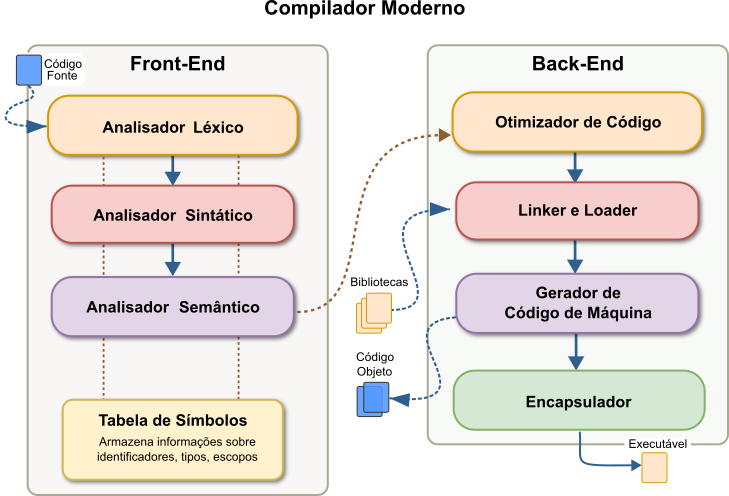
\includegraphics[width=0.8\textwidth]{Figuras/compiler.png}

    \legend{Fonte: \citeonline{alcantara2024}.}
\end{figure}

De modo conceitual, a operação de um compilador ocorre por meio de fases sequenciais, nas quais cada etapa tem o papel de converter o programa de um nível de abstração para outro. O núcleo de análise é formado pelas fases iniciais, que englobam as análises léxica, sintática e semântica. A partir desse ponto, o fluxo do compilador avança para as etapas de síntese, que englobam a geração do código intermediário, a otimização desse código e, por fim, a geração do código-alvo \cite{aho1995,cooper2012}.

A tabela de símbolos é gerenciada ao longo de todas essas fases. Trata-se de uma estrutura de dados muito importante para o compilador, pois mapeia todos os identificadores usados no programa fonte. Ao coletar e armazenar informações sobre os atributos de cada identificador, essa tabela permite recuperar escopos rapidamente e realizar a validação semântica durante a tradução \cite{aho1995,price2001}.

\subsection{O Modelo de Análise e Síntese (Fases da Compilação)}

De modo geral, a tradução é normalmente dividida em duas etapas principais: a análise e a síntese.
No estágio de análise (\textit{front-end}), o foco está em interpretar o programa original, dividindo-o em componentes menores para gerar uma abstração chamada representação intermediária.
Por outro lado, o estágio de síntese (\textit{back-end}) converte essa representação no programa final pretendido.
Essa distinção arquitetural entre \textit{front-end} e \textit{back-end} funciona como uma camada de abstração que simplifica a portabilidade, permitindo que o compilador suporte diversas linguagens e diferentes plataformas de hardware com maior agilidade \cite{aho1995,cooper2012}.

Para lidar com a complexidade da tradução de linguagens de alto nível, o fluxo operacional é dividido em unidades lógicas menores, chamadas de fases. Cada fase é responsável por uma transformação específica na representação do código. Na prática, essas fases podem ser agrupadas em ``passagens'' (\textit{passes}), estratégias que percorrem o código para otimizar a gerência de memória e o desempenho do sistema \cite{aho1995,cooper2012}.

As principais etapas que integram um compilador são detalhadas a seguir:

\begin{itemize}
    \item \textbf{Análise Léxica (\textit{Scanner}):} É a primeira etapa da compilação e processa o código-fonte caractere a caractere. Sua função é converter o fluxo de texto em uma sequência de unidades lógicas conhecidas como \textit{tokens}, removendo elementos irrelevantes para o processamento, como comentários e espaços redundantes \cite{cooper2012,nystrom2021}.

    \item \textbf{Análise Sintática (\textit{Parser}):} Utiliza a sequência de \textit{tokens} para validar a conformidade gramatical do programa em relação às regras da linguagem. O \textit{parser} organiza esses elementos em estruturas hierárquicas (as árvores sintáticas ou de derivação), empregando métodos descendentes (\textit{top-down}) ou redutivos (\textit{bottom-up}) \cite{aho1995,cooper2012}.

    \item \textbf{Análise Semântica:} Esta fase vai além da forma gramatical para garantir que as instruções tenham coerência lógica e operacional. Uma atividade importante aqui é a checagem de tipos (\textit{type checking}), que valida se a interação entre operadores, variáveis e funções respeita as definições da linguagem \cite{aho1995,cooper2012}.

    \item \textbf{Geração de Código Intermediário:} Concluídas as análises, o sistema produz uma versão do código que é independente da arquitetura final. O ``código de três endereços'' é um formato recorrente nesta etapa, servindo para reduzir a complexidade entre a abstração do alto nível e o rigor das instruções de máquina \cite{cooper2012,price2001}.

    \item \textbf{Otimização de Código:} Dedica-se ao refinamento do código intermediário, buscando torná-lo mais eficiente. O objetivo principal é reduzir o tempo de processamento e a ocupação de memória sem alterar o comportamento funcional do programa \cite{aho1995,cooper2012}.

    \item \textbf{Geração de Código Objeto:} Marca o encerramento da fase de síntese, na qual a representação intermediária é mapeada para a linguagem alvo (seja \textit{assembly} ou código de máquina). Esta etapa exige precisão na escolha das instruções nativas e cuidado na gestão dos registradores e endereços de memória do processador \cite{aho1995,cooper2012}.
\end{itemize}

Durante todo o ciclo, dois componentes dão suporte contínuo: o gerenciador da Tabela de Símbolos e o Tratador de Erros. A tabela de símbolos centraliza o registro de identificadores e seus metadados (como tipo e escopo), garantindo acesso rápido às informações em qualquer fase. Já o módulo de erros monitora falhas léxicas, sintáticas e lógicas, aplicando rotinas de recuperação que permitem ao compilador prosseguir com a análise e identificar o maior número possível de inconsistências em uma única execução \cite{aho1995,cooper2012}.

% ------------------------------------------------------------------------------------------------

\subsection{A Análise Léxica e o Reconhecimento de \textit{Tokens}}

Conhecida tecnicamente como \textit{scanner}, a análise léxica representa o estágio inicial do pipeline de compilação. Sua principal responsabilidade é percorrer o código-fonte caractere por caractere, processando essa entrada bruta para agrupar elementos em unidades com significado para a gramática da linguagem, chamadas de lexemas (conforme ilustrado na Figura \ref{fig:lexemas_nystrom}) \cite{cooper2012,nystrom2021}.

\begin{figure}[htb]
    \centering
    \caption{Exemplificação de agrupamento de caracteres em lexemas.}
    \label{fig:lexemas_nystrom}
    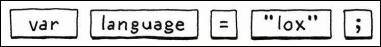
\includegraphics[width=0.8\textwidth]{Figuras/lex.png}
    \legend{Fonte: \citeonline[p. 43]{nystrom2021}.}
\end{figure}

Ao mesmo tempo em que organiza esses elementos, o analisador léxico realiza uma ``limpeza'' no fluxo de dados. Ele identifica e descarta componentes que, embora úteis ao programador, são irrelevantes para a tradução lógica, como comentários, tabulações e espaços em branco excedentes \cite{cooper2012,price2001}.

É importante, contudo, não confundir os conceitos de lexema e \textit{token}. O lexema refere-se à sequência literal de caracteres encontrada no texto original (a \textit{string} propriamente dita, como ``if'', ``soma'' ou ``42''). Já o \textit{token} é um objeto abstrato produzido pelo compilador para representar esse lexema. O \textit{token} carrega a categoria sintática da unidade (identificador, operador, palavra-chave) e, frequentemente, metadados adicionais, como o valor convertido e as coordenadas de linha e coluna, importantes para o rastreio de erros em fases posteriores \cite{cooper2012,nystrom2021}.

Para que o reconhecimento desses padrões ocorra de forma rigorosa, a micro-sintaxe da linguagem é definida por meio de expressões regulares. Esse modelo matemático permite descrever, de maneira concisa, as regras de formação de cada categoria de \textit{token}, definindo, por exemplo, quais combinações de símbolos formam um número real ou um nome de variável válido dentro daquela linguagem \cite{price2001,cooper2012}.

Contudo, expressões regulares são ferramentas de especificação, não de execução. Para que o computador processe essas regras, elas são convertidas em autômatos finitos. Um autômato funciona como uma máquina de estados: ele consome a entrada caractere por caractere, transitando entre estados lógicos até atingir um ``estado de aceitação''. Quando isso ocorre, o lexema é validado e o \textit{token} correspondente é enviado para o analisador sintático \cite{price2001,cooper2012}.

A implementação baseada em autômatos garante que a análise léxica seja eficiente, operando em tempo linear em relação ao volume de código. Na prática, desenvolvedores utilizam ferramentas de geração automática, como o \textit{Lex}, que transformam definições baseadas em expressões regulares diretamente em código otimizado de autômatos finitos determinísticos \cite{cooper2012,price2001}.

% ------------------------------------------------------------------------------------------------------------

\subsection{Estratégias de Análise Sintática: \textit{Top-Down} e \textit{Bottom-Up}}

A etapa de análise sintática, comumente chamada de \textit{parsing}, tem a tarefa de validar se a sequência de \textit{tokens} gerada previamente está de acordo com as regras gramaticais da linguagem de origem. Para processar essa estrutura e gerar a árvore de derivação, o sistema utiliza algoritmos baseados em duas abordagens principais: a análise descendente (\textit{top-down}), que atua da raiz para as folhas, e a análise ascendente (\textit{bottom-up}), que opera no sentido inverso \cite{aho1995,cooper2012}.

\noindent\textbf{I) Análise Sintática Descendente (\textit{Top-Down}):} Esta abordagem busca reconstruir a árvore sintática partindo do símbolo inicial (raiz) até alcançar os elementos terminais (folhas) que compõem o código de entrada. Durante esse fluxo, o analisador expande de forma sistemática o símbolo não-terminal posicionado mais à esquerda, utilizando as regras de produção para realizar o que se conhece tecnicamente como derivação à esquerda (\textit{leftmost derivation}) \cite{aho1995,price2001}.

Dentro dessa categoria, destacam-se os métodos recursivos descendentes e os preditivos baseados em tabelas, como o LL(1). O uso de analisadores por descida recursiva é frequente em projetos reais devido à sua legibilidade, simplicidade de implementação manual e eficiência no tratamento e diagnóstico de erros. Entretanto, para garantir um processamento linear e evitar o \textit{backtracking} (retrocesso), a gramática precisa ser cuidadosamente preparada: ela não deve apresentar recursão à esquerda e precisa ser devidamente fatorada. Isso assegura que o analisador consiga decidir qual regra aplicar consultando apenas o próximo \textit{token} da entrada \cite{cooper2012,nystrom2021}.

\noindent\textbf{II) Análise Sintática Ascendente ou Redutiva (\textit{Bottom-Up}):} Diferente do modelo anterior, a análise ascendente inicia o reconhecimento a partir dos \textit{tokens} individuais (folhas) e progride estruturalmente até atingir o símbolo inicial da gramática (raiz) \cite{aho1995,cooper2012}.

O termo ``redutiva'' caracteriza bem o funcionamento deste algoritmo: o analisador identifica padrões na pilha que correspondem ao lado direito de uma regra gramatical (denominados \textit{handles}) e os substitui (reduz) pelo respectivo símbolo não-terminal do lado esquerdo. Esse procedimento resulta em uma derivação à direita realizada de forma reversa \cite{aho1995,price2001}.

Os analisadores da família LR (como SLR, LALR e o LR Canônico) representam o que há de mais robusto nesta categoria, operando por meio de um sistema de empilhamento e redução (\textit{shift-reduce}) controlado por tabelas de estados. Uma vantagem significativa sobre a técnica descendente é a flexibilidade, pois os métodos \textit{bottom-up} lidam nativamente com recursão à esquerda e suportam quase todas as construções de gramáticas livres de contexto \cite{aho1995,cooper2012}.

Contudo, a criação manual das tabelas de transição para esses analisadores envolve alta complexidade matemática. Por esse motivo, a prática comum não envolve a codificação manual do \textit{parser}, mas sim o uso de ferramentas de geração automática, como o YACC, que traduzem a gramática formal diretamente em código funcional \cite{cooper2012,price2001}.

% -------------------------------------------------------------------------------------------------------------
\subsection{Análise Semântica e Verificação de Tipos}

Após a verificação gramatical feita pela análise sintática, o compilador entra na fase de análise semântica. Segundo \citeonline{price2001}, esta etapa tem como objetivo principal garantir que as estruturas e construções do programa, embora já validadas sintaticamente, façam sentido lógico para a posterior execução do código.
Enquanto o \textit{parser} (analisador sintático) assegura que a forma do código está correta, o analisador semântico vai além, inspecionando o que as peças do programa realmente significam de forma combinada \cite{nystrom2021}.
Nesse cenário, uma de suas atividades fundamentais é a resolução de associações, na qual o compilador verifica todas as variáveis mencionadas e determina exatamente a qual declaração de escopo cada identificador se refere \cite{nystrom2021}.

Outro componente central da análise semântica é a verificação de tipos \cite{aho1995, cooper2012}.
Nesta etapa, o compilador utiliza a estrutura hierárquica gerada previamente (a árvore de derivação) em conjunto com as informações coletadas na tabela de símbolos para checar se cada operador da linguagem está recebendo os operandos que lhe são legalmente permitidos \cite{aho1995}.
A análise semântica atua inferindo tipos para as expressões e detectando situações nas quais os valores são interpretados incorretamente \cite{cooper2012}.
Quando permitido pela especificação da linguagem, é também nesta fase que o compilador realiza conversões de tipo embutidas (coerções), como a transformação implícita de um valor inteiro para ponto flutuante antes de realizar uma adição entre tipos mistos \cite{aho1995, cooper2012}.

Os erros semânticos, por sua vez, são falhas peculiares, pois ocorrem em programas que podem possuir uma estrutura gramatical perfeitamente bem-formada, mas que violam as regras de significado, consistência ou contexto da linguagem de programação \cite{aho1995, cooper2012}.
O tratamento de erros semânticos é focado em capturar inconsistências que incluem, principalmente:

\begin{itemize}
    \item \textbf{Incompatibilidade de Tipos de Operandos:} Ocorre quando um operador é aplicado a um ou mais operandos cujos tipos de dados são conflitantes e não possuem regras de conversão implícita ou explícita \cite{aho1995, cooper2012}.
    Um exemplo prático na maioria das linguagens de programação fortemente tipadas é a tentativa inválida de se aplicar um operador aritmético binário a uma \textit{string} (texto) e a um booleano, ou tentar adicionar um tipo de precisão dupla a um tipo complexo de forma irregular \cite{cooper2012}.

    \item \textbf{Uso de Variáveis Não Declaradas ou Falhas de Escopo:} Este erro se manifesta quando o código faz referência a uma variável, função ou objeto que não foi previamente definido no programa, ou cuja declaração se encontra em um escopo léxico distinto e inacessível naquele momento \cite{cooper2012, nystrom2021}.
    A utilização de uma variável local fora de seu bloco restrito, por exemplo, acarretará uma falha semântica de identificador não reconhecido ou indefinido \cite{nystrom2021}.

    \item \textbf{Inconsistência de Aridade e Estruturas:} Acontece comumente em construções que exigem conformidade de números, como o número incorreto de argumentos \cite{cooper2012}.
    Exemplos incluem uma invocação de função ou chamada de procedimento na qual a quantidade de parâmetros passados difere da quantidade estipulada em sua definição original \cite{cooper2012, nystrom2021}.
    Igualmente, configura-se um erro semântico referenciar um \textit{array} informando um número de dimensões diferente do limite (ou \textit{rank}) estipulado em sua declaração \cite{cooper2012}.


\end{itemize}

% -------------------------------------------------------------------------------------------------------------

\subsection{Geração de Código Intermediário}

A fase de geração de código intermediário funciona como um mediador essencial entre a análise (\textit{front-end}) e a síntese (\textit{back-end}) de um sistema de compilação. Uma vez validadas as estruturas e a semântica do programa original, o compilador elabora uma representação interna explícita, projetada para ser agnóstica tanto em relação à linguagem de origem quanto à arquitetura de destino. Essa estratégia de tradução em múltiplos estágios é fundamental para decompor a complexidade de converter abstrações de alto nível em comandos de baixo nível de forma controlada. Além disso, essa camada de isolamento facilita a aplicação de técnicas de otimização e potencializa a portabilidade, visto que uma única representação interna pode ser mapeada para diferentes plataformas de \textit{hardware} \cite{cooper2012,price2001}.

Dentre os formatos de representação linear mais difundidos na literatura técnica, destaca-se o código de três endereços, que opera como um tipo de linguagem de montagem (\textit{assembly}) abstrata e universal. Nessa convenção, operações lógicas e aritméticas complexas são fragmentadas em instruções elementares contendo, no máximo, três operandos. A distinção crucial entre este formato e o código objeto final é que a representação intermediária ignora restrições físicas, como a gestão específica de registradores e o mapeamento direto de endereços de memória \cite{aho1995,cooper2012}.

Para exemplificar o conceito, considere uma expressão de atribuição como $A := X + Y * Z$. O compilador desmembra essa lógica em instruções de \textit{pseudo-assembly} simplificadas, utilizando variáveis temporárias para armazenar resultados parciais. O fluxo resultante em código de três endereços seguiria a sequência \cite{aho1995,cooper2012}:
\begin{enumerate}
    \item $T_1 := Y * Z$
    \item $T_2 := X + T_1$
    \item $A := T_2$
\end{enumerate}

A automação desse processo de conversão é viabilizada pela técnica de tradução dirigida pela sintaxe. Esse método expande o formalismo das gramáticas livres de contexto, permitindo que atributos sejam associados aos símbolos gramaticais e que ações semânticas específicas sejam vinculadas às regras de produção da linguagem \cite{aho1995,cooper2012}.

Na implementação prática, a emissão do código intermediário ocorre de forma síncrona com a análise sintática. No momento em que o \textit{parser} identifica uma construção gramatical legítima, ele dispara a ação semântica correspondente. Esse procedimento processa os atributos herdados ou sintetizados dos nós da árvore sintática, permitindo que os fragmentos de código sejam gerados de maneira ordenada e coerente com a lógica original do programa \cite{cooper2012,price2001}.

\subsection{Otimização de Código e Eficiência Computacional}

Posicionada estrategicamente como um estágio de refinamento no \textit{pipeline} de compilação, a otimização busca elevar a qualidade da representação interna do software. Esse aprimoramento vai além do ganho de velocidade e da economia de memória, abrangendo também a redução do consumo energético, um requisito crítico na computação contemporânea. Durante esta fase, o compilador atua substituindo construções genéricas por equivalentes semânticos mais ágeis. Um exemplo notório é o dobramento de constantes (\textit{constant folding}), que antecipa operações entre valores fixos ainda em tempo de compilação, eliminando o custo desse processamento durante a execução do programa \cite{aho1995,cooper2012}.

A legitimidade de qualquer transformação de código está condicionada a dois critérios imperativos: a preservação semântica (segurança) e a eficácia computacional (rentabilidade). O pilar da segurança determina que a lógica original do algoritmo deve permanecer inalterada, assegurando que a otimização não introduza efeitos colaterais. Já a rentabilidade exige que a alteração proporcione uma melhoria de desempenho real e mensurável, justificando o esforço computacional e o tempo adicional dedicados pelo compilador ao processo \cite{cooper2012,price2001}.

Quanto à abrangência das intervenções, a otimização é classificada em quatro níveis de profundidade:

\begin{itemize}
    \item \textbf{Otimização Local:} Restringe-se à análise de blocos básicos, isto é, sequências de instruções sem desvios de controle. Neste nível, utilizam-se frequentemente Grafos Acíclicos Dirigidos (GADs) para detectar e remover subexpressões redundantes e gerir variáveis locais de forma eficiente \cite{aho1995,cooper2012}.

    \item \textbf{Otimização Regional:} Expande o foco para conjuntos de blocos básicos, concentrando esforços prioritariamente em laços de repetição (\textit{loops}). Dado que a maior parte da carga de processamento ocorre nestes ciclos, melhorias como o deslocamento de código invariante geram impactos substanciais na performance global \cite{aho1995,cooper2012}.

    \item \textbf{Otimização Global (Intraprocedural):} Analisa o contexto integral de uma função ou procedimento. Por meio de estudos minuciosos do fluxo de dados, o compilador identifica oportunidades de simplificação que seriam invisíveis sob uma inspeção puramente local ou limitada \cite{aho1995,cooper2012}.

    \item \textbf{Otimização Interprocedural:} Atua no nível mais macro, transpondo as fronteiras entre diferentes módulos e sub-rotinas. Este escopo permite manobras agressivas como o \textit{inlining}, onde o corpo de uma função é integrado diretamente ao ponto de chamada, eliminando a sobrecarga (\textit{overhead}) associada ao desvio de execução e à gestão de pilhas de ativação \cite{aho1995,cooper2012}.
\end{itemize}

Na prática, a maioria das rotinas de otimização é dividida em duas etapas: uma fase de análise, dedicada ao mapeamento de dependências e do fluxo de controle, seguida por uma fase de transformação sintática, que efetivamente reescreve o código. Entre as técnicas mais usuais, destacam-se a eliminação de código morto (instruções inacessíveis ou inúteis), a simplificação de redundâncias aritméticas e a movimentação estratégica de cálculos para fora de zonas de alta repetição \cite{aho1995,cooper2012}.

\subsection{Geração de Código Objeto e Mapeamento de Arquitetura}

A fase de geração de código objeto (ou geração de código de máquina) representa a culminação do processo de compilação, consolidando as atividades finais do \textit{back-end}. O propósito central desta etapa é converter a representação intermediária otimizada na linguagem nativa da plataforma de destino. Para tanto, o compilador deve assegurar não apenas a fidelidade lógica em relação ao código original, mas também o aproveitamento máximo dos recursos de \textit{hardware} para garantir uma execução de alta performance \cite{aho1995,cooper2012}.

Um dos obstáculos primordiais nesta fase reside na acentuada heterogeneidade das arquiteturas de hardware. Cada família de processadores, a exemplo das arquiteturas x86, ARM ou RISC-V, possui sua própria Arquitetura do Conjunto de Instruções (ISA - \textit{Instruction Set Architecture}). Consequentemente, as operações de baixo nível e suas respectivas codificações binárias variam drasticamente entre diferentes sistemas, exigindo um mapeamento preciso para cada caso \cite{cooper2012,price2001}.

Para mitigar a complexidade de desenvolver um compilador do zero para cada novo processador, a engenharia de software moderna adota o princípio da \textit{retargetabilidade} (redirecionamento). Essa modularidade é viabilizada pelo papel central da representação intermediária: enquanto o \textit{front-end} opera de forma agnóstica em relação ao hardware, a adaptação para uma nova arquitetura exige apenas a substituição ou reconfiguração do módulo gerador de código (\textit{back-end}) \cite{aho1995,cooper2012}.

A síntese do código para uma máquina específica fundamenta-se em duas atividades interdependentes:

\begin{itemize}
    \item \textbf{Seleção de Instruções:} Atua como um mecanismo de reconhecimento de padrões que mapeia o fluxo do código intermediário para a sequência de comandos da ISA do processador que apresente o menor custo computacional possível \cite{aho1995,cooper2012}.
    \item \textbf{Alocação de Registradores:} Gerencia o conjunto limitado de registradores físicos da Unidade Central de Processamento (UCP). Esta tarefa é crítica, pois o compilador deve decidir estrategicamente quais valores devem permanecer nesses componentes de altíssima velocidade e quais devem ser transferidos para a memória principal (\textit{spilling}), visando minimizar os atrasos de acesso \cite{aho1995,cooper2012}.
\end{itemize}

% -----------------------------------------------------------------------------------------------------------
\subsection{Execução de Código de Máquina}

Ao término do processo de síntese, o que emerge é uma sucessão binária, densa e linear de operações primitivas. Diferente das abstrações hierárquicas manipuladas nas etapas iniciais da compilação, como as árvores sintáticas, o código de máquina é desprovido de estruturas de alto nível. Trata-se de uma linguagem de baixíssimo nível, constituída por instruções rudimentares que ocupam apenas alguns \textit{bytes} e ditam ações imediatas nos circuitos: movimentação de dados entre células de memória e registradores ou a execução de operações aritméticas básicas \cite{cooper2012,nystrom2021}.

Para que essa massa de dados binários ganhe vida, o programa deve ser transferido para a memória principal. Neste estágio, o sistema operacional, auxiliado por um \textit{software} carregador (\textit{loader}), prepara o ambiente de tempo de execução (\textit{runtime}). Este processo envolve a segmentação da memória em áreas distintas, isolando o setor de código estruturado das regiões destinadas ao armazenamento de dados \cite{cooper2012,price2001}.

A partir desse momento, o comando da execução passa à Unidade Central de Processamento (UCP). O ``guia'' dessa jornada é um registrador especializado da arquitetura, conhecido como Contador de Programa (\textit{Program Counter} - PC) ou Ponteiro de Instrução (\textit{Instruction Pointer} - IP), cuja função é monitorar rigorosamente o endereço da próxima instrução a ser processada \cite{cooper2012,price2001}.

A execução ocorre por meio de um ciclo mecânico e ininterrupto de busca e execução. O processador percorre a fita de instruções, decodifica o código de operação (\textit{opcode}) de cada entrada para extrair seu significado semântico e, em seguida, executa a tarefa correspondente. Nesse ecossistema de baixo nível, a complexidade dos laços de repetição e desvios condicionais das linguagens de alto nível é simplificada drasticamente. O controle do fluxo é resolvido exclusivamente através de operações de salto (\textit{jumps} ou \textit{branches}), que alteram o fluxo ao escrever um novo endereço de memória diretamente no Contador de Programa, desviando o ``foco'' da UCP de um ponto do binário para outro \cite{cooper2012,nystrom2021}.

%----------------------------------------------------------------------------------------------------------
\section{Engenharia de Software}
\label{sec:engenharia-software}

Esta seção reúne as práticas de engenharia de software que orientaram a construção da plataforma: a organização do trabalho em ciclos iterativos, a estratégia de testes automatizados, a separação de responsabilidades em camadas, as diretrizes de qualidade de código, a arquitetura do \textit{framework} adotado no \textit{front-end} e os princípios de experiência e interface do usuário.

\subsection{Desenvolvimento Iterativo e Incremental e \textit{Extreme Programming}}
\label{subsec:xp}

O gerenciamento clássico de projetos de software, frequentemente baseado no modelo em cascata (\textit{waterfall}), assume que o desenvolvimento pode ser tratado como uma sequência previsível e linear de atividades. No entanto, a engenharia de software lida com sistemas intrinsecamente complexos e com alto grau de incerteza, e o engessamento de requisitos em fases iniciais costuma resultar em desperdício e na entrega de produtos que não atendem às necessidades reais. Em contraponto a essa visão, o desenvolvimento iterativo e incremental assume a imprevisibilidade natural do processo e organiza o trabalho em ciclos curtos, nos quais o sistema cresce por acréscimos funcionais sucessivos, cada um integrado e verificado antes do início do seguinte \cite{agile2012,beck2004}.

Entre os métodos ágeis, o \textit{Extreme Programming} (XP) distingue-se por concentrar suas prescrições nas práticas técnicas de construção do software, e não em papéis ou cerimônias de gestão. O método parte do princípio de que o custo da mudança pode ser mantido baixo ao longo de todo o projeto, desde que o código permaneça simples, coberto por testes e continuamente refatorado. A mudança deixa, assim, de ser tratada como desvio a ser evitado e passa a ser incorporada ao fluxo normal de trabalho \cite{beck2004,wildt2015}.

As práticas que sustentam esse princípio incluem o planejamento incremental, no qual o escopo é detalhado apenas no momento em que será implementado; o \textit{design} simples, que evita antecipar estruturas ainda não exigidas; o desenvolvimento guiado por testes, que estabelece o comportamento esperado antes da implementação; a refatoração contínua, que preserva a legibilidade do código à medida que ele cresce; a integração contínua, que reduz o custo de reunir contribuições paralelas; e a propriedade coletiva do código, segundo a qual qualquer integrante pode alterar qualquer parte do sistema, sustentada pela revisão mútua entre os desenvolvedores \cite{beck2004,wildt2015}.

Essa combinação torna o XP particularmente adequado a equipes reduzidas, nas quais não há massa crítica para instanciar papéis especializados: os mesmos desenvolvedores acumulam as atribuições de levantamento de requisitos, projeto, implementação, teste e revisão. Nesse cenário, as práticas técnicas assumidas pelo método ocupam o lugar dos mecanismos de coordenação que métodos orientados a processo delegariam a papéis distintos \cite{wildt2015}. As subseções seguintes detalham três dessas práticas que estruturaram diretamente a construção da plataforma: os testes automatizados e o \textit{Test-Driven Development}, a separação de responsabilidades em camadas e as diretrizes de \textit{Clean Code}.

\subsection{Testes Automatizados e \textit{Test-Driven Development} (TDD)}
\label{subsec:testes-tdd}

A garantia da qualidade de um software exige validação contínua de seus comportamentos. Em projetos modernos, a automação de testes reduz a dependência de verificação manual e fornece uma rede de segurança para alterações, refatorações e evolução do código. Essa prevenção contra a quebra de comportamentos já consolidados é conhecida como teste de regressão; além de validar funcionalidades, os testes automatizados funcionam como documentação executável das regras de negócio do sistema \cite{aniche2012,silveira2012}.

Nesse contexto, o TDD inverte o ciclo tradicional de implementação, exigindo que o desenvolvedor escreva um teste automatizado antes da funcionalidade. O ciclo vermelho-verde-refatora consiste em criar primeiro um teste que falha, escrever o código mínimo para fazê-lo passar e, por fim, refatorar a solução mantendo o comportamento validado \cite{aniche2012,martin_coder}.

Mais do que uma técnica de verificação, o TDD também influencia o \textit{design} de software. Ao escrever o teste primeiro, o desenvolvedor precisa pensar na interface pública, nas dependências e na responsabilidade de cada componente; dificuldades excessivas na escrita dos testes podem indicar acoplamento elevado, baixa coesão ou problemas de arquitetura \cite{martin_clean,aniche2012}.

A estratégia de testes de um sistema costuma ser distribuída em diferentes níveis de granularidade, arranjo frequentemente ilustrado pela chamada pirâmide de testes. A base é composta pelos testes de unidade, rápidos e isolados, que verificam o comportamento de pequenas partes do código. O nível intermediário abriga os testes de integração, responsáveis por garantir a correta comunicação entre componentes e serviços de infraestrutura. No topo situam-se os testes de ponta a ponta (\textit{end-to-end}), que validam o sistema inteiro a partir da interface do usuário, ao custo de execuções mais lentas e frágeis. A recomendação decorrente é concentrar o maior volume de casos na base e reservar os níveis superiores para os fluxos mais críticos \cite{aniche2012,silveira2012}.

\subsection{Arquitetura Limpa e Separação de Responsabilidades}

O projeto arquitetural de um sistema deve separar responsabilidades em camadas com papéis independentes e bem definidos. A interface de usuário no \textit{front-end} concentra-se na experiência de uso e na integração visual, enquanto regras de negócio, persistência e serviços de apoio devem permanecer desacoplados de detalhes periféricos de entrega. Essa separação reduz dependências indevidas e facilita testes, manutenção e evolução do software \cite{martin_clean,silveira2012}.

No contexto da plataforma, a separação entre elementos de interface, regras de customização da linguagem, execução do código e persistência de dados contribui para que cada parte possa evoluir sem comprometer as demais. Essa organização também favorece o uso de padrões de projeto e abstrações voltadas à redução de acoplamento entre os módulos \cite{martin_clean}. Os padrões efetivamente adotados na construção da plataforma, bem como os pontos do código em que foram aplicados, são enumerados na Seção~\ref{sec:arquitetura-plataforma}.

\subsection{Qualidade de Código e \textit{Clean Code}}

A construção de um software de maneira ágil e sustentável esbarra invariavelmente na qualidade de sua base de código. O código-fonte é a linguagem formal na qual os requisitos de um sistema são expressos e detalhados de modo que a máquina possa executá-los. No entanto, sob a pressão de prazos, é comum que as equipes produzam códigos desorganizados, resultando em uma degradação estrutural contínua que, a longo prazo, faz a produtividade despencar, podendo até mesmo inviabilizar a evolução do projeto \cite{martin_clean_code,agile2012}.

Para combater essa entropia, a adoção das práticas de Código Limpo torna-se essencial. A escrita de um código limpo exige disciplina, o uso consciente de padrões e uma sensibilidade aguçada para reconhecer a desorganização e aplicar refatorações. Um código limpo deve ser elegante, simples, direto e, sobretudo, legível para os seres humanos. O profissionalismo no desenvolvimento de software pressupõe que o código não deve apenas funcionar, mas deve ser fácil de entender, alterar e estender por outros desenvolvedores \cite{martin_clean_code}.

Dentre as diretrizes estruturais básicas e inegociáveis para a manutenção dessa clareza na base de código, destacam-se \cite{martin_clean_code}:

\begin{itemize}
    \item \textbf{Nomes Significativos:} A nomenclatura de variáveis, funções, parâmetros e classes deve revelar claramente a sua intenção e responder ao porquê de sua existência e ao que o componente faz. Deve-se evitar o uso de siglas obscuras, codificações desnecessárias ou trocadilhos que exijam mapeamentos mentais, facilitando assim a leitura fluida e a busca no código \cite{martin_clean_code}.

    \item \textbf{Funções Pequenas e Focadas:} Uma função deve ser extremamente concisa e projetada para fazer estritamente uma única coisa, mantendo um único nível de abstração. Funções extensas que realizam múltiplas tarefas, agrupam várias seções lógicas ou que misturam tratamento de erros com a lógica de negócio violam a organização e dificultam o entendimento e a testabilidade \cite{martin_clean_code}.

    \item \textbf{Uso Consciente de Comentários:} O uso de comentários costuma compensar a incapacidade do programador de se expressar claramente através do próprio código. Eles não devem ser utilizados para encobrir ou justificar um código ruim ou confuso. A energia da equipe deve ser direcionada para tornar o código tão claro e autoexplicativo que elimine a necessidade de anotações redundantes \cite{martin_clean_code}.

    \item \textbf{Eliminação de Duplicidade e Refatoração contínua:} A repetição de código é o grande inimigo de um sistema bem desenvolvido, pois representa trabalho, risco e complexidade desnecessária. Deve-se melhorar o \textit{design} do código de forma contínua, aplicando refatorações que tornem o sistema mais enxuto e compreensível, sem alterar o seu comportamento externo \cite{martin_clean_code,agile2012}.
\end{itemize}

\subsection{O Framework Next.js e sua Arquitetura}

O Next.js é um \textit{framework} React voltado para a construção de aplicações web \textit{full-stack}, que facilita o desenvolvimento ao configurar internamente ferramentas de baixo nível, como empacotadores e compiladores, permitindo que o foco seja direcionado exclusivamente à construção do produto. A evolução de sua arquitetura ficou marcada pela transição do modelo tradicional de rotas, conhecido como \textit{Pages Router}, para o \textit{App Router}. Esse novo modelo adota uma arquitetura avançada centrada em \textit{React Server Components}, aprimorando o processo de busca de dados e permitindo o uso nativo de \textit{layouts} aninhados por meio de uma estrutura rigorosa de arquivos, utilizando convenções como \texttt{layout.tsx} e \texttt{loading.tsx} \cite{ziemann2025,vercel2024}.

A adoção de componentes de servidor transforma a forma de renderização, pois permite que o código seja executado exclusivamente no servidor e nunca seja enviado ao cliente, o que elimina a sobrecarga de arquivos JavaScript redundantes ao navegador. Integrado a essa estrutura arquitetural, o \textit{framework} disponibiliza o \textit{streaming}, uma técnica muitas vezes apoiada pelo \textit{React Suspense}, que permite enviar partes da interface gráfica progressivamente para o cliente à medida que os dados ficam prontos, reduzindo o tempo de espera inicial percebido pelo usuário \cite{lai2025,vercel2024}.

Outra característica de destaque, consolidada nas versões mais recentes, é o uso de \textit{Server Actions}. Tais ações consistem em funções assíncronas executadas diretamente no servidor que podem ser invocadas a partir de componentes interativos no cliente. Essa abordagem simplifica mutações de dados complexas, como submissões de formulários e interações com o banco de dados, eliminando a necessidade de criar arquivos manuais para \textit{endpoints} de API \cite{makerkit2026,vercel2024}.

Por fim, para a otimização em ambiente de produção, a ferramenta não apenas suporta múltiplas estratégias de renderização, como a estática e a dinâmica, mas também possibilita a escolha do ambiente de execução (\textit{runtime}) mais adequado para cada rota. O desenvolvedor pode optar pelo \textit{Node.js Runtime} padrão, que possui acesso completo a todas as APIs e ao ecossistema do Node.js, ou pelo \textit{Edge Runtime}, que opera com base em APIs da Web e é projetado para latência mínima e inicialização rápida ao lidar com lógicas de resposta simples \cite{makerkit2026,vercel2024}.

\subsection{Design de Experiência do Usuário (UX) e Interface do Usuário (UI)}
\label{subsec:uxui}

O \textit{design} de produtos digitais modernos compreende duas disciplinas fundamentais e complementares: a Experiência do Usuário (UX) e a Interface do Usuário (UI). A UX refere-se à percepção, às emoções e às respostas de um indivíduo ao interagir com um sistema ao longo de toda a sua jornada. Essa área vai muito além da usabilidade, englobando a compreensão profunda do comportamento, das necessidades e das frustrações do público-alvo. Para garantir uma boa experiência, a organização estrutural é essencial, sendo a Arquitetura da Informação a especialidade responsável por moldar, gerenciar e dispor os conteúdos de modo a tornar a navegação fluida, acessível e agradável \cite{seyffert2026,lima2024,raposo2012}.

Por outro lado, a UI diz respeito à camada visual e interativa com a qual o usuário interage diretamente. Isso inclui a definição rigorosa de leiautes, botões, tipografia, cores e componentes visuais. Mais do que atuar apenas na estética, uma interface bem projetada deve garantir clareza e consistência de uso. Uma organização confusa no aspecto visual pode comprometer toda a experiência global e levar ao abandono do sistema, independentemente de quão robusta seja a sua funcionalidade em \textit{back-end} \cite{seyffert2026,lima2024}.

A relação entre essas duas áreas é de forte complementaridade, na qual a UX estrutura a lógica e a solução do problema, enquanto a UI materializa essas soluções em uma interface tangível e eficiente. O desenvolvimento adequado em engenharia de software dita que a estruturação de UX anteceda a de UI; ou seja, define-se primeiramente quais problemas serão resolvidos e como os fluxos de navegação funcionarão, para somente então aplicar o \textit{design} visual \cite{seyffert2026,raposo2012}.

Essa intersecção técnica também é fortemente influenciada por aspectos cognitivos e leis da psicologia. O chamado ``efeito estética-usabilidade'', por exemplo, demonstra que os usuários tendem a perceber um \textit{design} esteticamente agradável, isto é, uma boa UI, como sendo inerentemente mais utilizável e eficiente na resolução de suas tarefas. Para avaliar e garantir a eficácia dessas interfaces, métodos de inspeção como a avaliação heurística são comumente aplicados. Trata-se de uma análise guiada por heurísticas (princípios gerais de bom \textit{design}) para certificar itens como a visibilidade do estado do sistema e a prevenção de erros, maximizando a usabilidade final do artefato \cite{yablonski2020,raposo2012}.

Um desdobramento operacional desses princípios é a acessibilidade da interface, normatizada pela especificação \textit{Accessible Rich Internet Applications} (WAI-ARIA), mantida pelo \textit{World Wide Web Consortium} \cite{w3c2023aria}. A especificação parte de uma constatação simples: os elementos nativos do HTML comunicam automaticamente seu significado às tecnologias assistivas, mas componentes ricos construídos com elementos genéricos (uma caixa de diálogo montada sobre \texttt{div}, por exemplo) chegam ao leitor de tela desprovidos de qualquer semântica. Para suprir essa lacuna, a WAI-ARIA define três categorias de atributos: os \textit{papéis} (\textit{roles}), que declaram o que um elemento é (diálogo, aba, menu, alerta); os \textit{estados}, que descrevem sua condição corrente e mutável (expandido, selecionado, desabilitado); e as \textit{propriedades}, que expressam relações estáveis entre elementos (qual rótulo descreve qual campo, qual região é controlada por qual botão). A especificação estabelece ainda requisitos de operação exclusivamente por teclado e de gerenciamento de foco, de modo que todo recurso acionável pelo ponteiro também o seja pela navegação sequencial, e que a posição do foco permaneça previsível quando a interface muda de estado \cite{w3c2023aria}.

\section{Softwares Educativos e Tecnologias de Apoio à Aprendizagem}

Uma plataforma educativa é um ambiente virtual desenvolvido para apoiar processos de ensino e aprendizagem, oferecendo recursos, ferramentas e conteúdos que facilitam a interação entre alunos, professores e instituições de ensino. Nesse cenário de transformação, a escolha da ferramenta certa não é apenas uma questão tecnológica, mas um fator determinante para o engajamento, a motivação e o sucesso educacional \cite{benedetti2025,mindmakers2025}.

Contudo, para aproveitar o potencial das novas tecnologias, a instituição de ensino precisa ir além da simples adoção de ferramentas digitais. É essencial entender o propósito pedagógico por trás de cada inovação, garantindo que a tecnologia esteja sempre a serviço da aprendizagem, e não o contrário. Afinal, a tecnologia educacional atua como um meio que exige professores preparados para usar recursos digitais de forma criativa e estratégica, conectando os alunos a um aprendizado relevante, dinâmico e significativo \cite{mindmakers2025}.

Quando projetada com esse foco pedagógico, uma plataforma educativa bem estruturada permite a personalização do aprendizado, ajustando-se ao ritmo e ao estilo de cada aluno, o que maximiza seu potencial e promove uma assimilação muito mais eficaz do conteúdo. Essa abordagem valoriza o tempo de cada estudante e amplia as suas capacidades ao longo de toda a jornada educacional. Ademais, a integração de dinâmicas interativas nas ferramentas de ensino, como a gamificação e a aprendizagem baseada em desafios, transforma a educação em um processo envolvente de recompensas. Esses sistemas lúdicos ajudam a despertar o interesse contínuo dos alunos e a desenvolver habilidades socioemocionais indispensáveis, como persistência e colaboração \cite{benedetti2025,mindmakers2025}.

\label{sec:softwares-apoio}

\section{Trabalhos Relacionados}
\label{sec:trabalhos-relacionados}

Esta seção tem como finalidade situar a plataforma desenvolvida neste trabalho no conjunto de soluções tecnológicas voltadas ao ensino introdutório de programação. Embora o objetivo do projeto seja apoiar a aprendizagem de programação, e não o ensino de construção de compiladores, sua própria natureza, a de uma IDE acoplada a um interpretador de gramática configurável, posiciona a proposta na fronteira entre dois universos de ferramentas: de um lado, os ambientes voltados à iniciação em programação; de outro, os projetos didáticos de construção de compiladores e de analisadores léxicos e sintáticos, cujas decisões técnicas e pedagógicas são pertinentes por dialogarem diretamente com o núcleo de tradução que sustenta esta plataforma. Por essa razão, são examinadas cinco iniciativas representativas do estado da arte, organizadas nas duas subseções seguintes conforme o grupo a que pertencem e observando, em cada uma delas, as escolhas de interface, os recursos pedagógicos e as estratégias de interação com o estudante. Ao final, apresenta-se uma análise comparativa que evidencia as lacunas restantes e o diferencial da abordagem proposta, que se situa justamente entre esses dois grupos.

\subsection{Ambientes Voltados à Iniciação em Programação}

Reúnem-se aqui as ferramentas cujo público-alvo é o estudante em primeiro contato com a programação e cujo propósito declarado é reduzir o atrito desse contato inicial. Cada uma é examinada segundo os três eixos anunciados no início desta seção: as escolhas de interface, os recursos pedagógicos e as estratégias de interação com o estudante.

\noindent\textbf{Portugol Studio e Portugol Webstudio}

\textit{Escolhas de interface.} Criado pelo Laboratório de Inovação Tecnológica na Educação (LITE) da Universidade do Vale do Itajaí, o Portugol Studio é distribuído como um ambiente de desenvolvimento integrado de código aberto, originalmente para instalação local. A migração posterior para o Portugol Webstudio transferiu edição, compilação e execução para o navegador, decisão que remove a barreira da instalação em laboratórios escolares com configurações heterogêneas. A composição da tela reproduz a organização convencional de uma IDE profissional, com editor central, painel de saída e área de inspeção, de modo que a familiaridade adquirida seja transferível a ferramentas de mercado \cite{gomes2020,univali2026}.

\textit{Recursos pedagógicos.} O recurso central é a própria linguagem: construções sintáticas inspiradas em C e PHP, porém com palavras-chave integralmente traduzidas para o português brasileiro, o que evita que o aprendiz lide com dois idiomas ao mesmo tempo durante o estudo das estruturas básicas de controle de fluxo e de dados. A esse núcleo somam-se um depurador com execução passo a passo, um inspetor de variáveis sincronizado com a linha em execução e uma árvore que representa a estrutura sintática do código produzido, recursos que tornam observável o que normalmente permanece implícito para o iniciante \cite{gomes2020,univali2026}.

\textit{Estratégias de interação.} A interação apoia-se na visualização do programa em funcionamento: o estudante acompanha, linha a linha, a alteração dos valores em memória, o que aproxima a execução mental do algoritmo de sua execução efetiva. O suporte nativo a bibliotecas gráficas e sonoras amplia essa estratégia ao permitir projetos lúdicos, como pequenos jogos, cuja saída visível fornece retorno imediato sobre o efeito do código escrito \cite{martins2025,univali2026}.

\noindent\textbf{Quorum: linguagem de programação baseada em evidências}

\textit{Escolhas de interface.} O ecossistema disponibiliza o Quorum Studio, IDE concebida desde o início para operar com leitores de tela, e não adaptada a eles posteriormente. O ambiente funciona tanto em modo \textit{offline}, com geração de \textit{bytecode} para a máquina virtual Java, quanto em modo executável no navegador, o que permite adotá-lo em contextos com restrições de instalação \cite{quorum2025,ladner2019}.

\textit{Recursos pedagógicos.} O traço distintivo do projeto é submeter as decisões de sintaxe e de semântica a verificação empírica, em vez de herdá-las por imitação ou familiaridade histórica. Os testes conduzidos pela equipe responsável compararam linguagens consolidadas no mercado a uma linguagem de controle cujas palavras-chave foram geradas aleatoriamente, recurso metodológico que isolou o efeito da forma sintática sobre o desempenho de novatos. As evidências indicaram que substituir símbolos como chaves, colchetes e pontos e vírgulas por palavras de vocabulário comum reduz de modo consistente as taxas de erro sintático, resultado visível em construções como \texttt{repeat 10 times}, cuja leitura se aproxima de uma instrução em linguagem natural \cite{stefik2013}.

\textit{Estratégias de interação.} A modalidade primária de interação prevista é auditiva: a linguagem foi desenhada para que sua leitura por síntese de voz permaneça inteligível, o que condiciona desde a escolha das palavras-chave até a pontuação. O ecossistema estende essa interação a domínios de saída variados --- áudio, gráficos e robótica ---, oferecendo ao estudante formas de perceber o resultado do programa que não dependem exclusivamente da leitura visual de texto \cite{quorum2025,ladner2019}.

\noindent\textbf{Beecrowd: prática de algoritmos e avaliação automatizada}

\textit{Escolhas de interface.} Antes denominada URI Online Judge, a Beecrowd é uma plataforma inteiramente web, organizada em torno de um catálogo de problemas navegável por tema e por nível de dificuldade. A interface não oferece ambiente de desenvolvimento: o estudante escreve a solução em ferramenta externa e submete o código pronto, o que pressupõe que ele já disponha de um ambiente configurado \cite{ferreira2025}.

\textit{Recursos pedagógicos.} O acervo contempla milhares de problemas categorizados, abrangendo desde estruturas básicas de seleção e repetição até tópicos avançados como grafos e programação dinâmica, e admite submissões em diversas linguagens consolidadas no mercado, incluindo C++, Python, Java e JavaScript. A graduação de dificuldade é o principal recurso didático, pois permite ao estudante progredir por incrementos e ao professor selecionar conjuntos coerentes com o momento da disciplina \cite{ferreira2025,maonocodigo2022}.

\textit{Estratégias de interação.} A dinâmica articula-se em torno de um ciclo curto de submissão e \textit{feedback}: o estudante lê o enunciado, redige uma solução e a envia ao sistema, que a executa contra um conjunto fechado de casos de teste e retorna, em poucos segundos, um veredito como ``\textit{Accepted}'', ``\textit{Wrong Answer}'' ou ``\textit{Presentation Error}''. Cabe observar que esse retorno é binário quanto ao resultado e não localiza o erro no código. Combinado a elementos de gamificação como \textit{rankings} públicos, fóruns e contagem de submissões aceitas, o ciclo sustenta um regime de prática deliberada que tende a manter o estudante em posição ativa \cite{ferreira2025,garcia2024}.

\subsection{Projetos Didáticos de Construção de Compiladores}

Reúnem-se aqui as iniciativas voltadas ao ensino da construção de tradutores. Embora se dirijam a um público mais avançado, suas decisões técnicas e pedagógicas dialogam diretamente com o núcleo de tradução que sustenta a plataforma proposta, e por isso são examinadas segundo os mesmos três eixos.

\noindent\textbf{Laila: gerador de analisadores léxicos e sintáticos \textit{online}}

\textit{Escolhas de interface.} A ferramenta oferece um ambiente de desenvolvimento inteiramente executado no navegador, construído em JavaScript com o \textit{framework} VueJS e apoiado na biblioteca CodeMirror, responsável pelo destaque de sintaxe e pela sinalização \textit{inline} de inconsistências. A camada de \textit{back-end} é uma API REST em Python que coordena a execução de FLEX e Bison no servidor. Essa escolha responde a um problema concreto de interface com a disciplina: a instalação coordenada desses geradores junto a uma cadeia compatível do GCC consome parte significativa da carga horária de laboratório, sobretudo em sistemas operacionais que não derivam do Linux \cite{ladgelson2021}.

\textit{Recursos pedagógicos.} O recurso didático central é a possibilidade de o estudante especificar gramáticas, redigir analisadores léxicos e sintáticos e executar os experimentos sem qualquer dependência local, concentrando o tempo de aula no objeto de estudo e não em sua configuração. O servidor captura comportamentos anômalos, como laços infinitos ou erros de compilação, e devolve os diagnósticos correspondentes ao cliente \cite{ladgelson2021}.

\textit{Estratégias de interação.} A interação organiza-se em um ciclo curto entre edição, submissão e retorno do resultado. Estudos de caso conduzidos junto a turmas de Ciência da Computação relataram ganhos perceptíveis de engajamento e de compreensão prática dos algoritmos de análise, atribuídos justamente à brevidade desse ciclo \cite{ladgelson2021}.

\noindent\textbf{\textit{chibicc}: abordagem incremental para o ensino de compiladores}

\textit{Escolhas de interface.} Este é o caso em que a análise por eixos revela a maior distância em relação às demais ferramentas: o \textit{chibicc} não possui interface própria. Trata-se de um repositório de código-fonte, cuja fruição pressupõe editor, cadeia de compilação e sistema de controle de versão já instalados e dominados pelo estudante. Toda a mediação recai sobre o histórico de \textit{commits} do projeto \cite{ueyama2020}.

\textit{Recursos pedagógicos.} O traço pedagógico mais relevante está na organização incremental. Em vez de expor o aprendiz, desde o princípio, a uma arquitetura completa com múltiplos passes e estruturas internas elaboradas, o projeto propõe uma trajetória gradual em que cada etapa adiciona uma única capacidade gramatical ou semântica ao compilador. O ponto de partida é um tradutor mínimo que reconhece apenas um número como entrada válida; sobre essa base, são integrados, em iterações sucessivas, suporte a expressões, declarações, controle de fluxo, ponteiros, estruturas e demais elementos do C11. Apesar do enfoque didático, o resultado cobre parte expressiva da especificação C11, sendo capaz de compilar, sem adaptações, projetos de complexidade considerável, como o sistema de controle de versão Git e o gerenciador de banco de dados SQLite \cite{ueyama2020}.

\textit{Estratégias de interação.} Não há retorno automatizado nem execução assistida: a interação consiste na leitura do código de cada etapa e em sua reimplementação pelo estudante, que verifica o próprio progresso executando manualmente a suíte de testes do projeto. A estratégia favorece a observação direta da relação entre escolhas de implementação e comportamento do compilador, mas transfere integralmente ao aprendiz a responsabilidade pela regulação do próprio ritmo \cite{ueyama2020}.

\subsection{Análise Crítica e o Diferencial da Solução Proposta}

A Tabela~\ref{tab:comparativo} sintetiza as principais características das ferramentas examinadas frente à plataforma proposta, evidenciando, em especial, a personalização da sintaxe pelo próprio estudante como traço distintivo da abordagem.

\begin{landscape}
\begin{table}[p]
    \centering
    \caption{Comparativo entre as ferramentas analisadas e a plataforma proposta, segundo os três eixos de análise.}
    \label{tab:comparativo}
    \footnotesize
    \setlength{\tabcolsep}{4pt}
    \renewcommand{\arraystretch}{1.3}
    \begin{tabular}{|>{\raggedright\arraybackslash}p{2.3cm}|>{\raggedright\arraybackslash}p{4.3cm}|>{\raggedright\arraybackslash}p{4.7cm}|>{\raggedright\arraybackslash}p{4.7cm}|>{\raggedright\arraybackslash}p{4.4cm}|}
        \hline
        \textbf{Ferramenta} & \textbf{Escolhas de interface} & \textbf{Recursos pedagógicos} & \textbf{Estratégias de interação} & \textbf{Personalização da sintaxe pelo estudante} \\
        \hline
        Portugol Studio e Webstudio
          & IDE própria, em versão local e em versão executada no navegador
          & Linguagem com palavras-chave em português; depurador, inspetor de variáveis e árvore sintática
          & Acompanhamento visual da execução; projetos gráficos e sonoros
          & Não \\
        \hline
        Quorum
          & IDE própria concebida para leitores de tela; execução local ou no navegador
          & Sintaxe definida por evidência empírica; operadores expressos por palavras
          & Leitura por síntese de voz; saídas em áudio, gráficos e robótica
          & Não \\
        \hline
        Beecrowd
          & Plataforma web sem ambiente de edição; exige ferramenta externa
          & Acervo graduado por tema e dificuldade; múltiplas linguagens de mercado
          & Ciclo submissão--veredito, sem localização do erro; gamificação
          & Não \\
        \hline
        Laila
          & IDE web com destaque de sintaxe e diagnóstico \textit{inline}
          & Dispensa a instalação de FLEX, Bison e GCC, liberando o tempo de laboratório
          & Ciclo curto entre edição, execução e diagnóstico
          & Sim, mas como objeto de estudo: o aluno escreve gramáticas formais \\
        \hline
        \textit{chibicc}
          & Sem interface própria; repositório de código-fonte
          & Trajetória incremental, uma capacidade da linguagem por etapa
          & Leitura e reimplementação do código; sem retorno automatizado
          & Não \\
        \hline
        \textbf{Plataforma proposta}
          & IDE web própria, com terminal integrado e sistema de arquivos
          & Exposição das fases de tradução (\textit{tokens} e código intermediário); avaliação automatizada de exercícios
          & Execução e depuração passo a passo; erros relatados no vocabulário escolhido pelo próprio estudante
          & Sim: palavras-chave, delimitadores de bloco, operadores, literais booleanos e terminador de instrução \\
        \hline
    \end{tabular}
    \legend{Fonte: elaborado pelo autor.}
\end{table}
\end{landscape}

Quando observadas em conjunto, as ferramentas analisadas organizam-se em dois grandes grupos cujas limitações afetam diretamente o público iniciante. O primeiro grupo reúne soluções dedicadas à prática algorítmica e à formação inicial em programação, do qual fazem parte o Portugol Studio, o Quorum e a Beecrowd. Embora apresentem avanços relevantes, seja por meio da tradução das palavras-chave para o português, da adoção de uma sintaxe baseada em evidências ou da prática contínua sustentada por avaliação automatizada, todas operam sob uma gramática fixa, definida previamente pelos seus responsáveis. O estudante permanece, portanto, na condição de quem se adapta à linguagem, e não de quem participa de sua modelagem; pequenas diferenças entre o vocabulário esperado e o vocabulário internalizado podem invalidar soluções logicamente corretas e reintroduzir, ainda que de forma reduzida, a barreira sintática que se buscava remover.

O segundo grupo reúne plataformas e projetos voltados ao ensino de compiladores propriamente dito, exemplificados pela Laila e pelo \textit{chibicc}. Ambos oferecem contribuições expressivas em seus nichos, sobretudo na eliminação do atrito de configuração ou na apresentação incremental da arquitetura de um compilador. Contudo, o público pressuposto é, em grande medida, o de estudantes em estágio avançado de cursos de Computação, com domínio prévio de linguagens estritas como C11 e de geradores como FLEX e Bison, o que afasta esses recursos do estudante que ainda enfrenta a barreira inicial de entrada no pensamento computacional.

A plataforma proposta situa-se entre esses dois grupos. Em vez de oferecer uma gramática previamente fixada ou de exigir a configuração local de cadeias de ferramentas, este trabalho disponibiliza uma IDE web integrada a um interpretador dinâmico cuja função principal é deslocar o controle estrutural da linguagem para o próprio estudante. Por meio da interface, é possível redefinir palavras-chave, delimitadores de bloco, operadores expressos por palavras, literais booleanos e regras de finalização de instrução, sem que o aprendiz precise lidar com a complexidade interna das fases de análise léxica, sintática e semântica.

Do ponto de vista da experiência do usuário, a personalização oferecida pela plataforma transforma o ato de programar em uma atividade na qual a linguagem se ajusta ao repertório do aprendiz, e não o contrário. Esse arranjo cria um laboratório seguro de experimentação algorítmica, no qual a frustração associada a erros de digitação ou de memorização de palavras reservadas é substituída pela investigação consciente das estruturas de controle e de dados. Forma-se, assim, uma ponte pedagógica entre a primeira aproximação ao raciocínio computacional e o futuro contato do estudante com as linguagens estritas e com os juízes automatizados que predominam no mercado e nas etapas mais avançadas da formação.


\chapter{PROPOSTA} \label{cap:proposta}

A finalidade deste capítulo é delimitar o que se pretende construir ao longo das duas fases do Trabalho de Conclusão de Curso e, em seguida, apresentar a cadeia temporal de atividades prevista na pré-proposta aprovada. A descrição parte da plataforma vista como produto educacional, atravessa as macroatividades técnicas necessárias à sua materialização e culmina na exposição do cronograma e do regime de trabalho em dupla adotado.

O artefato que orienta este trabalho não é apenas um compilador ou um editor de código, mas sim uma plataforma educacional web cuja unidade de valor é a possibilidade de o estudante personalizar a própria linguagem que utilizará para aprender programação. Em termos concretos, oferece-se ao usuário a possibilidade de redefinir o vocabulário das palavras-chave, escolher os delimitadores de bloco que melhor representem sua noção de escopo, substituir operadores lógicos e relacionais por palavras de uso natural, reescrever os literais booleanos no idioma de sua preferência e ajustar as regras de finalização de instrução. Cada uma dessas dimensões responde, em alguma medida, a uma fonte conhecida de atrito sintático no contato inicial com linguagens consolidadas no mercado, sendo a sua reunião sob uma mesma interface o que sustenta o caráter inovador da proposta. A Tabela~\ref{tab:elementos-configuraveis} detalha cada um desses elementos, confrontando a forma canônica herdada da família C com um exemplo de personalização e com as restrições verificadas pela plataforma no momento da configuração.

\begin{table}[htbp]
    \centering
    \caption{Elementos da linguagem passíveis de redefinição pelo usuário.}
    \label{tab:elementos-configuraveis}
    \footnotesize
    \setlength{\tabcolsep}{4pt}
    \renewcommand{\arraystretch}{1.25}
    \begin{tabular}{|>{\raggedright\arraybackslash}p{2.5cm}|>{\raggedright\arraybackslash}p{2.6cm}|>{\raggedright\arraybackslash}p{2.9cm}|>{\raggedright\arraybackslash}p{5.2cm}|}
        \hline
        \textbf{Elemento} & \textbf{Forma canônica} & \textbf{Exemplo de personalização} & \textbf{Restrições verificadas} \\
        \hline
        Palavras-chave de tipo & \texttt{int}, \texttt{float}, \texttt{bool}, \texttt{string} & \texttt{inteiro}, \texttt{real}, \texttt{logico}, \texttt{texto} & Devem ter forma de identificador e não colidir entre si nem com os demais elementos configurados \\
        \hline
        Controle de fluxo & \texttt{if}, \texttt{else}, \texttt{for}, \texttt{while}, \texttt{break}, \texttt{continue}, \texttt{return} & \texttt{se}, \texttt{senao}, \texttt{para}, \texttt{enquanto}, \texttt{pare}, \texttt{siga}, \texttt{retorne} & Mesmas restrições das palavras-chave de tipo \\
        \hline
        Entrada e saída & \texttt{print}, \texttt{scan} & \texttt{escreva}, \texttt{leia} & Mesmas restrições das palavras-chave de tipo \\
        \hline
        Operadores lógicos & \texttt{\&\&}, \texttt{||}, \texttt{!} & \texttt{e}, \texttt{ou}, \texttt{nao} & Forma de identificador; sem duplicatas; não podem reusar palavra reservada nem colidir com delimitadores de bloco \\
        \hline
        Operadores relacionais & \texttt{==}, \texttt{!=}, \texttt{>}, \texttt{>=}, \texttt{<}, \texttt{<=} & \texttt{igual}, \texttt{diferente}, \texttt{maior}, \texttt{maiorIgual}, \texttt{menor}, \texttt{menorIgual} & Mesmas restrições dos operadores lógicos \\
        \hline
        Literais booleanos & \texttt{true}, \texttt{false} & \texttt{verdadeiro}, \texttt{falso} & Forma de identificador; sem duplicatas; não podem conflitar com operadores em forma de palavra nem com delimitadores \\
        \hline
        Delimitadores de bloco & \texttt{\{} e \texttt{\}} & \texttt{inicio} e \texttt{fim}, ou indentação & Ambos preenchidos, com forma de identificador, distintos entre si e sem reusar palavra reservada \\
        \hline
        Terminador de instrução & \texttt{;} & \texttt{ponto} ou ausência de terminador & Não pode ser vazio, conter espaços, reusar o ponto e vírgula ou caracteres de operadores fixos, nem colidir com palavras já definidas na linguagem \\
        \hline
    \end{tabular}
    \legend{Fonte: elaborado pelo autor, a partir das funções de validação do módulo \texttt{config.ts} do pacote \texttt{compiler}.}
\end{table}


O conjunto completo de funcionalidades previstas para a plataforma, com os respectivos atores, é apresentado no diagrama de casos de uso da Figura~\ref{fig:casos-de-uso}. O diagrama distingue quatro atores: o visitante, que apenas se cadastra e se autentica; o usuário autenticado, que concentra as funcionalidades comuns de personalização da linguagem e de uso do ambiente de desenvolvimento; e os papéis de aluno e de professor, que dele herdam e acrescentam, respectivamente, as funcionalidades de participação em turmas e de gestão pedagógica.

\begin{landscape}
\begin{figure}[p]
    \centering
    \caption{Diagrama de casos de uso da plataforma.}
    \label{fig:casos-de-uso}
    \resizebox{\linewidth}{!}{%
    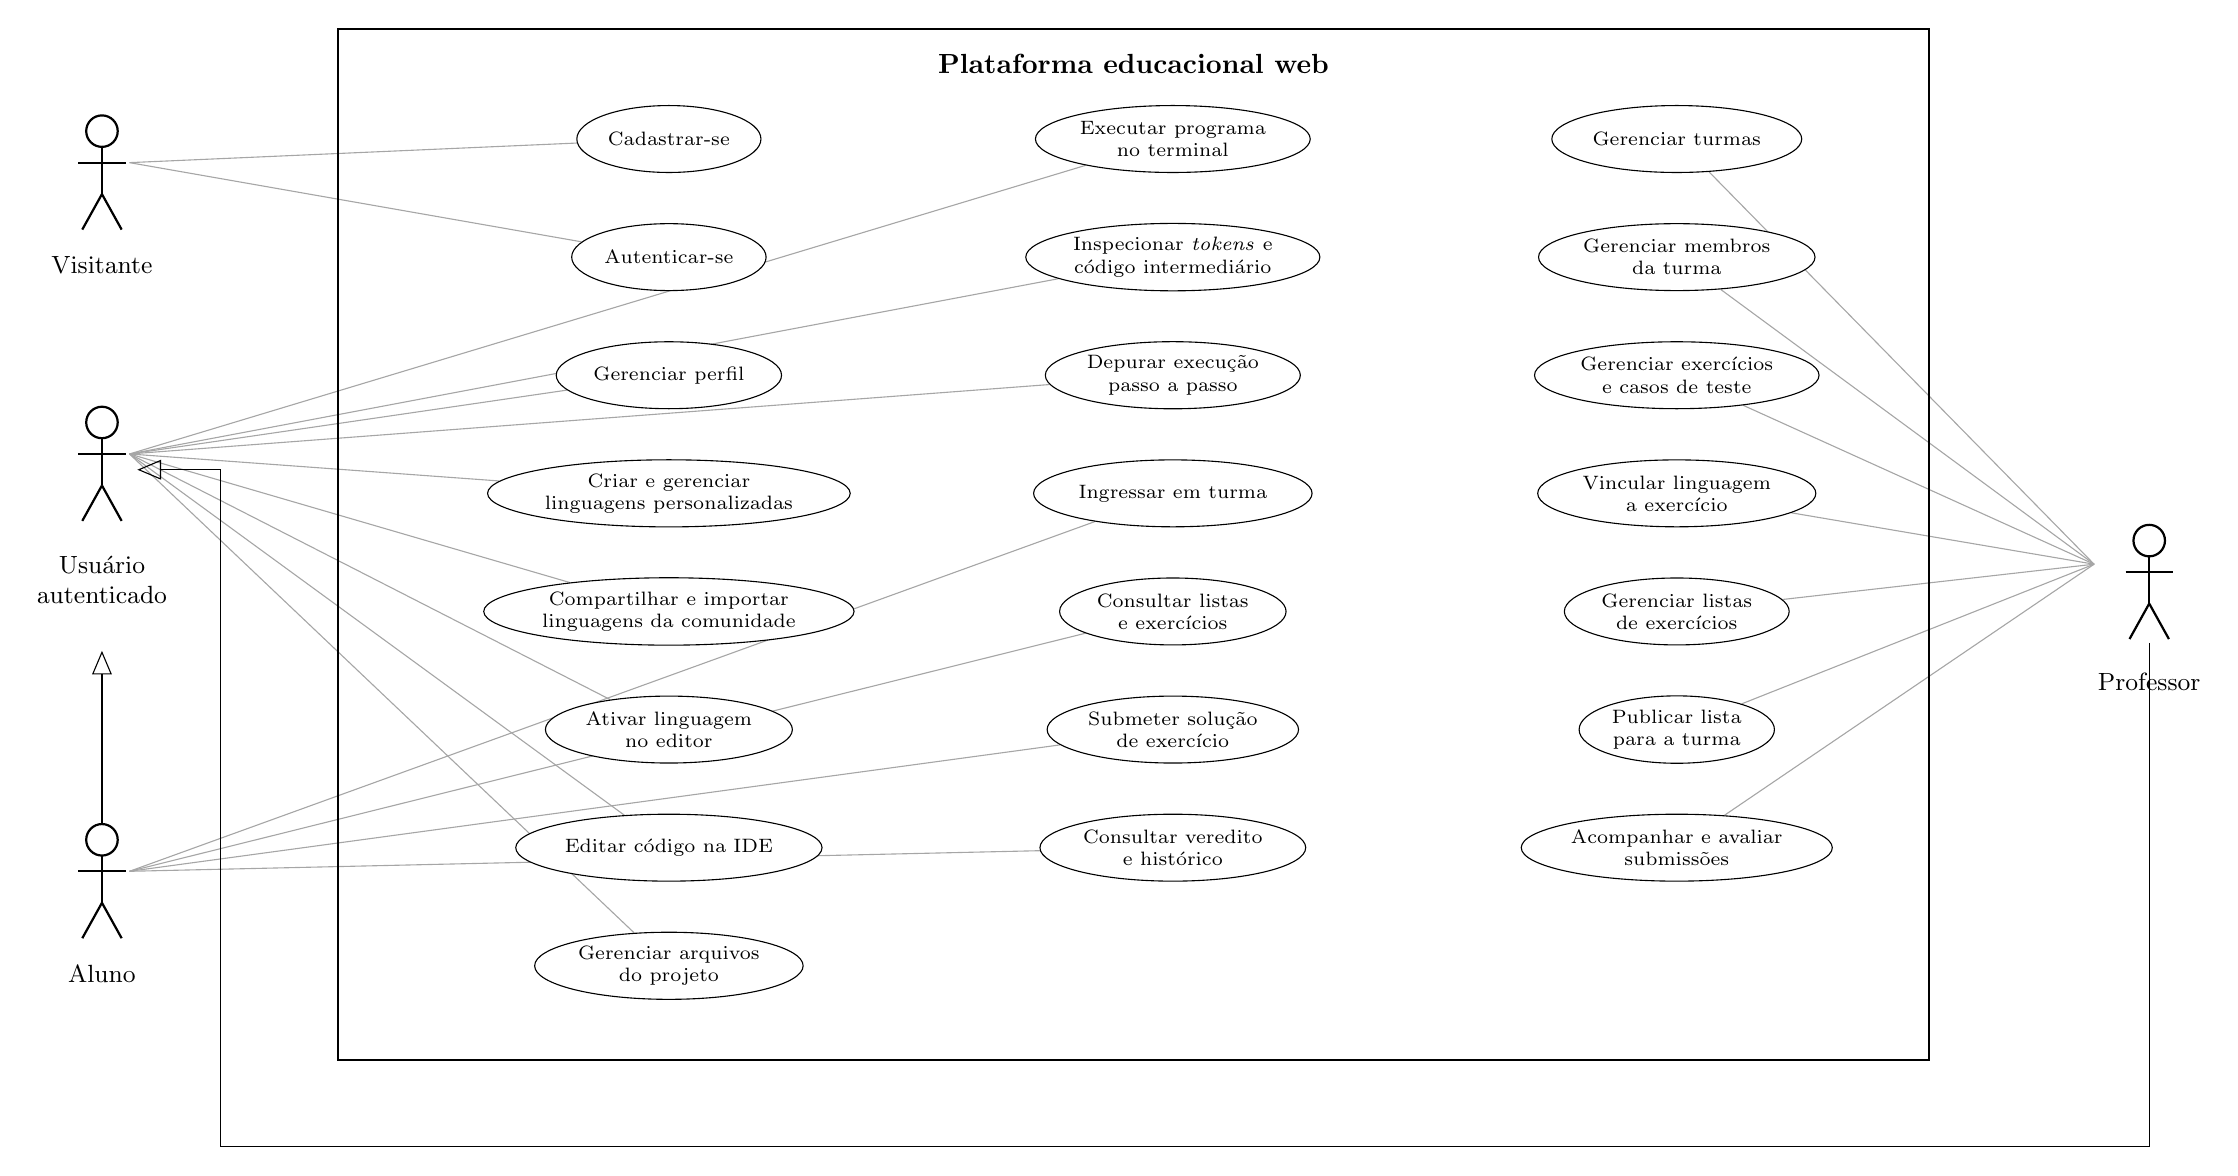
\begin{tikzpicture}[x=1cm,y=1cm]

    %% ---------- fronteira do sistema ----------
    \draw[thick] (3.0,5.9) rectangle (23.2,-7.2);
    \node[font=\bfseries, anchor=north] at (13.1,5.7) {Plataforma educacional web};

    %% ---------- atores ----------
    \pic at (0,4.6) {ator};  \node[font=\small, align=center] at (0,2.9) {Visitante};
    \pic at (0,0.9) {ator};  \node[font=\small, align=center] at (0,-1.1) {Usuário\\autenticado};
    \pic at (0,-4.4) {ator}; \node[font=\small, align=center] at (0,-6.1) {Aluno};
    \pic at (26.0,-0.6) {ator};  \node[font=\small, align=center] at (26.0,-2.4) {Professor};

    %% generalizacao: Aluno e Professor sao Usuarios autenticados.
    %% A do Professor e roteada abaixo da fronteira para nao cruzar os casos de uso.
    \draw[heranca] (0,-4.2) -- (0,-2.0);
    \draw[heranca] (26.0,-1.9) -- (26.0,-8.3) -- (1.5,-8.3) -- (1.5,0.3) -- (0.45,0.3);

    %% ---------- coluna A: acesso, conta e linguagem ----------
    \node[uc] (ucCad)  at (7.2, 4.5)  {Cadastrar-se};
    \node[uc] (ucAut)  at (7.2, 3.0)  {Autenticar-se};
    \node[uc] (ucPer)  at (7.2, 1.5)  {Gerenciar perfil};
    \node[uc] (ucLing) at (7.2, 0.0)  {Criar e gerenciar\\linguagens personalizadas};
    \node[uc] (ucCom)  at (7.2,-1.5)  {Compartilhar e importar\\linguagens da comunidade};
    \node[uc] (ucAtiv) at (7.2,-3.0)  {Ativar linguagem\\no editor};
    \node[uc] (ucEdit) at (7.2,-4.5)  {Editar código na IDE};
    \node[uc] (ucArq)  at (7.2,-6.0)  {Gerenciar arquivos\\do projeto};

    %% ---------- coluna B: ambiente de desenvolvimento e aluno ----------
    \node[uc] (ucExec) at (13.6, 4.5) {Executar programa\\no terminal};
    \node[uc] (ucTok)  at (13.6, 3.0) {Inspecionar \textit{tokens} e\\código intermediário};
    \node[uc] (ucDep)  at (13.6, 1.5) {Depurar execução\\passo a passo};
    \node[uc] (ucIng)  at (13.6, 0.0) {Ingressar em turma};
    \node[uc] (ucCons) at (13.6,-1.5) {Consultar listas\\e exercícios};
    \node[uc] (ucSub)  at (13.6,-3.0) {Submeter solução\\de exercício};
    \node[uc] (ucVer)  at (13.6,-4.5) {Consultar veredito\\e histórico};

    %% ---------- coluna C: gestao pedagogica ----------
    \node[uc] (ucTur)  at (20.0, 4.5) {Gerenciar turmas};
    \node[uc] (ucMem)  at (20.0, 3.0) {Gerenciar membros\\da turma};
    \node[uc] (ucEx)   at (20.0, 1.5) {Gerenciar exercícios\\e casos de teste};
    \node[uc] (ucVinc) at (20.0, 0.0) {Vincular linguagem\\a exercício};
    \node[uc] (ucLis)  at (20.0,-1.5) {Gerenciar listas\\de exercícios};
    \node[uc] (ucPub)  at (20.0,-3.0) {Publicar lista\\para a turma};
    \node[uc] (ucAva)  at (20.0,-4.5) {Acompanhar e avaliar\\submissões};

    %% ---------- associacoes (camada de fundo: passam atras das elipses) ----------
    \begin{scope}[on background layer]
      \foreach \d in {ucCad,ucAut}
        \draw[liga] (0.35,4.2) -- (\d);
      \foreach \d in {ucPer,ucLing,ucCom,ucAtiv,ucEdit,ucArq,ucExec,ucTok,ucDep}
        \draw[liga] (0.35,0.5) -- (\d);
      \foreach \d in {ucIng,ucCons,ucSub,ucVer}
        \draw[liga] (0.35,-4.8) -- (\d);
      \foreach \d in {ucTur,ucMem,ucEx,ucVinc,ucLis,ucPub,ucAva}
        \draw[liga] (25.3,-0.9) -- (\d);
    \end{scope}

    \end{tikzpicture}}
    \legend{Fonte: elaborado pelo autor.}
\end{figure}
\end{landscape}

A partir desses casos de uso, consolidaram-se os requisitos que orientaram a construção da plataforma. A Tabela~\ref{tab:requisitos-funcionais} relaciona os requisitos funcionais, isto é, o que o sistema deve fazer; a Tabela~\ref{tab:requisitos-nao-funcionais}, os requisitos não funcionais, que estabelecem as qualidades esperadas da solução e os critérios sob os quais ela será verificada.

\begin{table}[htbp]
    \centering
    \caption{Requisitos funcionais da plataforma.}
    \label{tab:requisitos-funcionais}
    \footnotesize
    \setlength{\tabcolsep}{4pt}
    \renewcommand{\arraystretch}{1.15}
    \begin{tabular}{|c|>{\raggedright\arraybackslash}p{12.3cm}|}
        \hline
        \textbf{ID} & \textbf{Descrição} \\
        \hline
        RF01 & Permitir o cadastro e a autenticação de usuários, distinguindo os papéis de aluno e de professor \\
        \hline
        RF02 & Permitir ao usuário autenticado consultar e editar os dados de seu perfil \\
        \hline
        RF03 & Oferecer um assistente guiado, organizado em etapas independentes, para a criação de uma linguagem personalizada \\
        \hline
        RF04 & Permitir a redefinição dos elementos da linguagem relacionados na Tabela~\ref{tab:elementos-configuraveis} \\
        \hline
        RF05 & Validar preventivamente cada configuração, impedindo colisões entre palavras-chave, operadores, literais, delimitadores e terminador de instrução \\
        \hline
        RF06 & Exibir, em tempo real, a pré-visualização de um programa exemplo sob a configuração corrente \\
        \hline
        RF07 & Persistir localmente a customização ativa e remotamente as linguagens nomeadas pelo usuário \\
        \hline
        RF08 & Permitir publicar uma linguagem no catálogo comunitário e importar linguagens publicadas por terceiros \\
        \hline
        RF09 & Oferecer edição de código com realce de sintaxe e sugestão automática ajustados à linguagem ativa \\
        \hline
        RF10 & Manter um sistema de arquivos virtual que permita criar, renomear, remover e alternar entre arquivos \\
        \hline
        RF11 & Executar o programa produzido no editor, com entrada e saída conectadas ao terminal integrado \\
        \hline
        RF12 & Exibir ao usuário a tabela de \textit{tokens} reconhecidos e o código intermediário gerado \\
        \hline
        RF13 & Oferecer execução passo a passo, destacando no editor a instrução em processamento \\
        \hline
        RF14 & Relatar erros léxicos, sintáticos, semânticos e de execução no vocabulário da linguagem ativa e no idioma selecionado \\
        \hline
        RF15 & Permitir ao professor criar e gerir turmas, e ao aluno ingressar em uma turma \\
        \hline
        RF16 & Permitir ao professor criar e gerir exercícios, com casos de teste de entrada e saída esperada \\
        \hline
        RF17 & Permitir vincular uma configuração de linguagem a um exercício, restringindo o vocabulário disponível ao aluno \\
        \hline
        RF18 & Permitir organizar exercícios em listas e publicá-las para uma turma \\
        \hline
        RF19 & Avaliar automaticamente a submissão do aluno contra os casos de teste do exercício \\
        \hline
        RF20 & Permitir ao professor acompanhar as submissões da turma e atribuir nota \\
        \hline
    \end{tabular}
    \legend{Fonte: elaborado pelo autor.}
\end{table}

\begin{table}[htbp]
    \centering
    \caption{Requisitos não funcionais da plataforma.}
    \label{tab:requisitos-nao-funcionais}
    \footnotesize
    \setlength{\tabcolsep}{4pt}
    \renewcommand{\arraystretch}{1.15}
    \begin{tabular}{|c|>{\raggedright\arraybackslash}p{12.3cm}|}
        \hline
        \textbf{ID} & \textbf{Descrição} \\
        \hline
        RNF01 & \textbf{Acessibilidade:} os componentes de interface devem observar as diretrizes WAI-ARIA \cite{w3c2023aria}, com navegação por teclado, leitura por tecnologias assistivas e gerenciamento de foco \\
        \hline
        RNF02 & \textbf{Responsividade:} as composições de tela devem reorganizar-se conforme a faixa de resolução do dispositivo \\
        \hline
        RNF03 & \textbf{Internacionalização:} toda cadeia visível ao usuário deve estar externalizada, com suporte aos idiomas \textit{pt-BR}, \textit{pt-PT}, \textit{es} e \textit{en} \\
        \hline
        RNF04 & \textbf{Autonomia de execução:} edição, análise léxica e sintática, geração de código intermediário e interpretação devem permanecer funcionais na ausência de conexão com o serviço de persistência \\
        \hline
        RNF05 & \textbf{Latência:} a execução do núcleo de tradução deve ocorrer sem ciclo de requisição e resposta a servidor remoto \\
        \hline
        RNF06 & \textbf{Consistência visual:} os temas claro e escuro devem manter paridade de contraste e legibilidade, inclusive no editor \\
        \hline
        RNF07 & \textbf{Testabilidade:} as construções críticas devem ser cobertas por testes automatizados, executados localmente e no \textit{pipeline} de integração contínua \\
        \hline
        RNF08 & \textbf{Segregação de acesso:} as rotas e operações restritas devem verificar o papel do usuário antes de permitir o acesso \\
        \hline
    \end{tabular}
    \legend{Fonte: elaborado pelo autor.}
\end{table}


Conforme definido na pré-proposta, a metodologia foi organizada em seis macroetapas complementares. Essas etapas não devem ser entendidas como blocos completamente isolados, pois o desenvolvimento de uma plataforma interativa exige revisões sucessivas entre interface, interpretador e experiência de uso. Ainda assim, elas delimitam com clareza o percurso técnico e acadêmico do projeto:

\begin{itemize}
    \item \textbf{Revisão bibliográfica:} levantamento das bases conceituais sobre interpretadores, compiladores e ferramentas educacionais relacionadas, com o objetivo de sustentar tanto as decisões de projeto quanto a posterior análise comparativa;
    \item \textbf{Definição de requisitos e arquitetura:} consolidação dos elementos configuráveis da linguagem, da modelagem das camadas da plataforma e dos contratos de comunicação entre o núcleo do interpretador e a IDE;
    \item \textbf{Desenvolvimento da plataforma:} implementação da aplicação web, contemplando os fluxos de edição, navegação, personalização, autenticação e uso educacional da IDE;
    \item \textbf{Implementação da análise dinâmica léxica e sintática:} integração entre o código escrito na IDE e as fases de reconhecimento de \textit{tokens} e validação sintática com suporte às regras configuradas pelo usuário;
    \item \textbf{Geração e interpretação do código intermediário:} disponibilização, no ambiente da IDE, da execução do código intermediário e do retorno de avisos, erros e resultados ao usuário;
    \item \textbf{Integração e testes entre plataforma e interpretador:} validação dos fluxos principais, com atenção à consistência da experiência, à acessibilidade, à responsividade e à preparação para os estudos com usuários.
\end{itemize}

A distribuição temporal dessas atividades ao longo dos doze meses que compreendem o TCC~I e o TCC~II é apresentada na Tabela~\ref{tab:cronograma}, conforme o cronograma registrado na pré-proposta. Cada coluna numerada corresponde a um mês corrido das duas etapas e cada célula marcada com ``X'' sinaliza a previsão de execução da respectiva atividade no período indicado.

\begin{table}[H]
    \centering
    \caption{Cronograma de desenvolvimento do trabalho de conclusão de curso.}
    \label{tab:cronograma}
    \footnotesize
    \setlength{\tabcolsep}{4pt}
    \renewcommand{\arraystretch}{1.2}
    \resizebox{\textwidth}{!}{%
    \begin{tabular}{|p{6.5cm}|c|c|c|c|c|c|c|c|c|c|c|c|}
        \hline
        \multirow{2}{*}{\textbf{Atividade}} & \multicolumn{6}{c|}{\textbf{TCC I}} & \multicolumn{6}{c|}{\textbf{TCC II}} \\
        \cline{2-13}
         & \textbf{01} & \textbf{02} & \textbf{03} & \textbf{04} & \textbf{05} & \textbf{06} & \textbf{07} & \textbf{08} & \textbf{09} & \textbf{10} & \textbf{11} & \textbf{12} \\
        \hline
        Revisão Bibliográfica & X & X & X & X & & & & & & & & \\
        \hline
        Escrita da Introdução e Revisão de Literatura & & X & X & X & & & & & & & & \\
        \hline
        Predefinição de escopo e Especificação dos comandos dinâmicos & & & X & X & & & & & & & & \\
        \hline
        Escrita da Metodologia & & & X & & X & X & & & & & & \\
        \hline
        Arquitetura e Modelagem da Plataforma & & & X & X & & & & & & & & \\
        \hline
        Customização dinâmica de \textit{tokens} e sintaxe & & & & X & X & & & & & & & \\
        \hline
        Execução da Análise Léxica e Sintática com o código da IDE & & & & & X & X & & & & & & \\
        \hline
        Execução do código intermediário no Terminal da IDE com \textit{feedback} (avisos e erros) & & & & & & X & X & X & & & & \\
        \hline
        Finalização de fluxos, acessibilidade e responsividade & & & & & & X & X & X & & & & \\
        \hline
        Testes, Validação com Usuários e Coleta de \textit{Feedback} & & & & & & & & & X & X & X & \\
        \hline
        Escrita do TCC (Resultados, Discussão e Conclusão) & & & & & & & & & X & X & X & X \\
        \hline
    \end{tabular}%
    }
    \legend{Fonte: elaborado pelo autor.}
\end{table}

Convém retomar, neste ponto, o regime de trabalho em dupla já apresentado na introdução (Capítulo~\ref{cap:introducao_modelo}), dada sua influência direta sobre o escopo do projeto e sobre os capítulos subsequentes. A pré-proposta aprovada para este Trabalho de Conclusão de Curso prevê a \textbf{participação conjunta em todas as etapas} do desenvolvimento, mas com funções complementares. Em respeito a esse compromisso, as decisões de arquitetura, os ciclos de revisão de código e as etapas de integração foram conduzidos de modo colaborativo pelos dois integrantes da dupla. Cabe ressaltar que, por se tratar de uma equipe reduzida, não houve especialização de papéis: ambos os integrantes acumularam as atribuições de levantamento de requisitos, projeto, implementação, teste e revisão. Adotaram-se, de forma pragmática, as práticas técnicas do \textit{Extreme Programming} discutidas no referencial teórico, sem ciclos de duração fixa: partiu-se de um conjunto mínimo de requisitos e o sistema avançou por acréscimos funcionais, incorporando as melhorias identificadas durante a própria implementação \cite{beck2004,wildt2015}.

A partir dessa base comum, a divisão complementar de eixos de aprofundamento manifesta-se nos capítulos de redação acadêmica e nas evoluções incrementais subsequentes. No presente documento, o autor concentra a investigação na plataforma e na customização de comandos: arquitetura da aplicação web, concepção do assistente de personalização, experiência de uso da IDE, execução do código no terminal integrado e procedimentos de coleta de \textit{feedback} junto aos estudantes. O detalhamento aprofundado da evolução do núcleo do interpretador, incluindo a geração de código intermediário e sua integração técnica ao restante da plataforma, é desenvolvido em paralelo pelo estudante Victor de Souza Vilela da Silva. Essa divisão de eixos não fragmenta o produto: o que se distribui é a profundidade analítica de cada autor sobre partes específicas do mesmo artefato, conduzido pelos dois em todas as etapas. Tal arranjo justifica-se pela amplitude do escopo, que, individualmente, tenderia a resultar em um interpretador simplificado ou em uma plataforma incompleta, restrita a um terminal.

Concluídas as etapas cobertas por este documento, dedicadas à fundamentação teórica, à modelagem da plataforma, à customização dinâmica de \textit{tokens} e sintaxe, à execução das análises léxica e sintática a partir da IDE e à execução do código intermediário no terminal integrado, a fase subsequente direcionará seus esforços à consolidação da plataforma e à definição do protocolo de avaliação: os instrumentos de coleta, as métricas e os critérios que permitirão, posteriormente, aferir em que medida a personalização da linguagem contribui para a aprendizagem. A aplicação desse protocolo junto a estudantes, com a consequente coleta de evidências empíricas em sala de aula, não integra o escopo deste trabalho e é registrada como encaminhamento futuro. O próximo capítulo, dedicado à modelagem, descreve o estado em que o sistema se encontra ao término do TCC~I.


\chapter{METODOLOGIA} \label{cap:metodologia}

Este capítulo apresenta a abordagem metodológica adotada para o desenvolvimento da plataforma web proposta neste trabalho, detalhando a arquitetura do Ambiente de Desenvolvimento Integrado (IDE), as estratégias empregadas para a customização dinâmica de tokens e sintaxe, os mecanismos de integração com o núcleo do interpretador e os fluxos de execução, avaliação e \textit{feedback} ao usuário. A condução do trabalho seguiu rigorosamente as etapas previstas no cronograma do projeto, contemplando, nesta primeira fase do Trabalho de Conclusão de Curso, a revisão bibliográfica, a especificação do escopo dos comandos dinâmicos, a modelagem da arquitetura da plataforma, a implementação da customização interativa da linguagem, a execução das análises léxica e sintática a partir do código produzido na IDE, a apresentação dos resultados intermediários no terminal embutido e a finalização dos fluxos principais, com atenção à acessibilidade e à responsividade.

O desenvolvimento foi conduzido de forma incremental e iterativa, em conformidade com os princípios do desenvolvimento ágil discutidos por \citeonline{agile2012} e \citeonline{sabbagh2014}. Em razão da elevada quantidade de telas, componentes interativos e estados compartilhados característicos de uma IDE web, cada fluxo da plataforma, desde a autenticação do usuário até a submissão de exercícios, foi tratado como uma unidade autônoma de entrega, modelada, implementada e validada antes da agregação à etapa seguinte. Essa abordagem foi sustentada por testes automatizados unitários e de integração escritos com o \textit{framework} Vitest, conforme as práticas de Desenvolvimento Guiado por Testes consolidadas por \citeonline{aniche2012} e \citeonline{martin_coder}, permitindo a verificação contínua de regressões diante das frequentes mudanças impostas pela natureza altamente interativa da plataforma.

\section{Modelagem da Arquitetura da Plataforma}
\label{sec:arquitetura-plataforma}

A organização da plataforma foi concebida sob a ótica da Separação de Responsabilidades defendida por \citeonline{martin_clean}, dividindo o projeto em três camadas independentes e bem delimitadas: o pacote \texttt{compiler}, responsável pelo núcleo do interpretador; o pacote \texttt{ide}, responsável pela camada de apresentação e por toda a interação com o usuário; e o serviço de \textit{back-end}, responsável pela persistência das entidades de domínio do Ambiente Virtual de Aprendizagem. Os pacotes \texttt{compiler} e \texttt{ide} são versionados em um único repositório no formato \textit{monorepo}, viabilizando o consumo direto do compilador como dependência local da IDE, sem qualquer empacotamento intermediário e sem comunicação remota entre as duas camadas. Essa decisão arquitetural reduz drasticamente a latência da execução de programas no navegador e simplifica a propagação de mudanças no compilador para a interface.

O \textit{front-end} foi implementado com o \textit{framework} Next.js, em sua arquitetura de \textit{Pages Router}, sobre a biblioteca React 19, utilizando TypeScript em todo o código-fonte para garantir a verificação estática de tipos discutida por \citeonline{martin_clean_code}. A estilização foi conduzida com Tailwind CSS em sua quarta versão, complementada por componentes acessíveis das bibliotecas \textit{shadcn/ui} e \textit{Radix UI}, escolhidos por implementarem as recomendações da \textit{Web Accessibility Initiative} (WAI-ARIA) por padrão. O gerenciamento de estado assíncrono foi delegado à biblioteca \textit{TanStack React Query}, responsável pela orquestração de cache, sincronização e revalidação dos dados consumidos das rotas HTTP, enquanto a validação de formulários foi modelada com a biblioteca \textit{Zod}, integrada ao \textit{React Hook Form}.

A camada de \textit{back-end} foi implementada em Python sobre o \textit{framework} FastAPI, escolhido pelas características de alto desempenho, validação automática via \textit{Pydantic} e geração automatizada de documentação OpenAPI discutidas por \citeonline{fastapi2026}. A persistência foi sustentada pelo ORM SQLAlchemy assíncrono, com versionamento de \textit{schema} via Alembic, isolando o modelo de dados das regras de negócio em conformidade com os princípios de Arquitetura Limpa apresentados por \citeonline{martin_clean}. Essa separação garante que o banco de dados seja tratado estritamente como um detalhe de infraestrutura, permitindo que o núcleo de compilação e a interface web permaneçam agnósticos em relação à camada de armazenamento.

O fluxo geral de comunicação entre as camadas, ilustrado pela Figura \ref{fig:arquitetura-plataforma}, foi estruturado de modo que a execução do código submetido pelo usuário ocorra integralmente nos limites do servidor Next.js. A IDE invoca rotas HTTP locais sob o caminho \texttt{/api}, que importam diretamente as classes \texttt{Lexer}, \texttt{TokenIterator} e \texttt{Interpreter} do pacote \texttt{compiler}. As requisições destinadas à persistência são, por sua vez, delegadas ao serviço FastAPI por meio do cliente HTTP \textit{axios}. Essa segregação confere à plataforma a flexibilidade de executar programas mesmo na ausência de conexão com o serviço de persistência, mantendo plenamente funcionais os recursos de edição, análise léxica, geração de código intermediário e interpretação.

\begin{figure}[H]
    \centering
    \caption{Arquitetura geral da plataforma e fluxos de comunicação entre as camadas.}
    \label{fig:arquitetura-plataforma}
    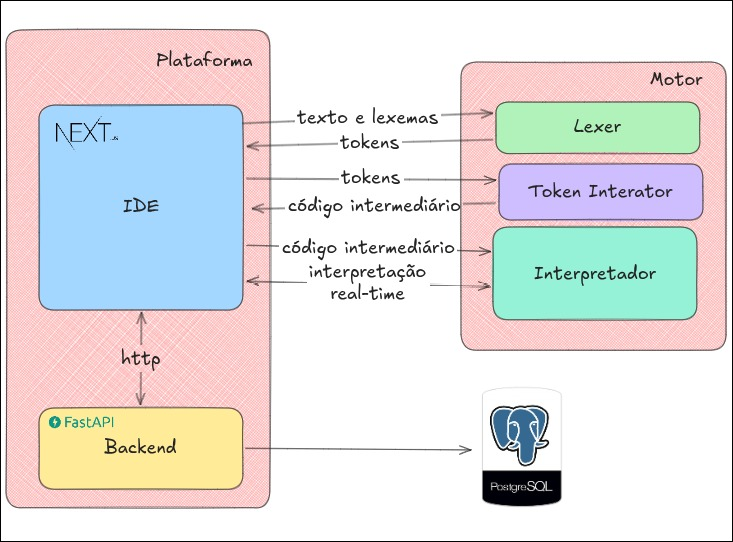
\includegraphics[width=0.95\textwidth]{Figuras/arquitetura-plataforma.jpeg}
    \legend{Fonte: elaborado pelo autor.}
\end{figure}

A organização interna do código da IDE seguiu a topologia clássica de aplicações Next.js, com diretórios dedicados para páginas (\texttt{pages}), componentes reutilizáveis (\texttt{components}), \textit{contexts} de estado global (\texttt{contexts}), \textit{hooks} personalizados (\texttt{hooks}), entidades de domínio (\texttt{entities}), bibliotecas de apoio (\texttt{lib}) e composições de tela (\texttt{views}). Essa segmentação materializa o princípio da coesão funcional discutido por \citeonline{silveira2012}, isolando responsabilidades específicas em módulos compactos e favorecendo tanto a legibilidade quanto a testabilidade do sistema.

\section{Interpretador}
\label{sec:interpretador-nucleo}

O interpretador constitui o núcleo de tradução comum a este projeto e foi desenvolvido de forma colaborativa pelos dois autores, Victor de Souza Vilela da Silva e Igor Lamoia Queiroz, conforme a divisão de responsabilidades registrada no Apêndice~\ref{ap:plano}. Implementado em TypeScript e consumido pela IDE como dependência local, conforme descrito na Seção~\ref{sec:arquitetura-plataforma}, o núcleo encadeia as fases de análise léxica, análise sintática, geração de código intermediário em três endereços e execução pelo interpretador, recebendo dinamicamente a configuração da linguagem definida pelo usuário (palavras-chave, operadores em forma de palavra, literais booleanos, delimitadores de bloco e terminador de instrução).

Por se tratar da base técnica compartilhada entre os dois volumes, o detalhamento interno de cada fase do núcleo, incluindo as estratégias de varredura léxica, a análise sintática por descida recursiva, a geração de código de três endereços e o funcionamento do interpretador, é objeto do trabalho complementar de autoria de Victor de Souza Vilela da Silva. Este volume concentra-se na forma como a IDE aciona e integra esse núcleo, detalhada nas seções seguintes.

\section{Customização Dinâmica de Tokens e Sintaxe}
\label{sec:customizacao-dinamica}

A funcionalidade central da plataforma, que consiste na possibilidade de o usuário personalizar dinamicamente a sintaxe e o vocabulário da linguagem, foi materializada em um conjunto coordenado de componentes, \textit{contexts} e utilitários. O elemento central dessa funcionalidade é o \texttt{KeywordContext}, um \textit{context} do React que mantém, em memória e na camada de armazenamento local do navegador, o estado completo da customização ativa, incluindo o mapeamento de palavras-chave personalizadas, os operadores em forma de palavra, os literais booleanos, os delimitadores de bloco e o terminador de instrução.

O contrato técnico que sustenta a customização é definido pelo módulo \texttt{config.ts} do pacote \texttt{compiler}, que declara, por meio de tipos TypeScript, todos os elementos da linguagem passíveis de personalização. O Trecho de Código~\ref{lst:lexer-config} apresenta esses tipos, que funcionam como a interface formal entre a camada de interface, responsável pela coleta das preferências do usuário, e o núcleo do tradutor, responsável pela construção da gramática efetiva no momento da varredura léxica.

\begin{lstlisting}[language=typescript, caption={Tipos que descrevem a configuração customizável do lexer.}, label={lst:lexer-config}, captionpos=b]
export type KeywordMap = Record<string, number>;

export type OperatorWordMap = {
  logical_or?: string;     logical_and?: string;
  logical_not?: string;    less?: string;
  less_equal?: string;     greater?: string;
  greater_equal?: string;  equal_equal?: string;
  not_equal?: string;
};

export type BooleanLiteralMap = {
  true?: string;
  false?: string;
};

export type LexerBlockDelimiters = {
  open: string;
  close: string;
};

export type LexerConfig = {
  customKeywords?: KeywordMap;
  operatorWordMap?: OperatorWordMap;
  booleanLiteralMap?: BooleanLiteralMap;
  statementTerminatorLexeme?: string;
  blockDelimiters?: LexerBlockDelimiters;
  locale?: string;
  indentationBlock?: boolean;
  tabWidth?: number;
};
\end{lstlisting}

A definição de quais elementos da linguagem seriam exibidos como configuráveis foi guiada pelos achados empíricos de \citeonline{stefik2013}, segundo os quais a sintaxe tradicional derivada da família C atua como uma barreira significativa para estudantes iniciantes. Foram disponibilizadas para customização as palavras-chave de declarações de tipo (\texttt{int}, \texttt{float}, \texttt{bool}, \texttt{string}), de controle de fluxo (\texttt{if}, \texttt{else}, \texttt{for}, \texttt{while}, \texttt{break}, \texttt{continue}, \texttt{return}, \texttt{switch}, \texttt{case}), as operações de entrada e saída (\texttt{print}, \texttt{scan}), os operadores lógicos (\texttt{\&\&}, \texttt{||}, \texttt{!}) e relacionais (\texttt{==}, \texttt{!=}, \texttt{>}, \texttt{>=}, \texttt{<}, \texttt{<=}), os literais booleanos (\texttt{true}, \texttt{false}), os delimitadores de bloco (chaves ou indentação) e o terminador de instrução. Essas opções abrangem precisamente os elementos que oneram a carga cognitiva inicial discutidos por \citeonline{stefik2013}, mantendo intactos os aspectos estruturais responsáveis pela consistência das demais fases do compilador.

A consolidação do estado da customização no \texttt{KeywordContext} é exposta às demais camadas da aplicação por meio do utilitário \texttt{buildLexerConfig}, apresentado no Trecho de Código~\ref{lst:build-lexer-config}. Esse utilitário traduz o estado em memória, contendo os mapeamentos de palavras-chave, os operadores, os literais booleanos, os delimitadores de bloco e o terminador de instrução, em um descritor compatível com o tipo \texttt{LexerConfig} do pacote \texttt{compiler}, atuando como a fronteira efetiva entre o estado da interface e a invocação do tradutor.

\begin{lstlisting}[language=typescript, caption={Utilitário \texttt{buildLexerConfig} do \texttt{KeywordContext}, que materializa a configuração corrente em um descritor consumível pelo lexer.}, label={lst:build-lexer-config}, captionpos=b]
const buildKeywordMap = useCallback((): Record<string, number> => {
  const map: Record<string, number> = {};
  for (const m of customization.mappings) {
    map[m.custom] = m.tokenId;
  }
  return map;
}, [customization.mappings]);

const buildLexerConfig = useCallback((): IDECompilerConfigPayload => {
  return buildLexerConfigFromCustomization(customization);
}, [customization]);
\end{lstlisting}

A interface de customização foi implementada como um assistente progressivo no formato \textit{wizard}, materializado no componente \texttt{keyword-customizer}, que conduz o usuário por etapas independentes, cada uma responsável por um aspecto específico da personalização. O fluxo é controlado pelo \texttt{wizard-model}, que mantém o estado de navegação e valida cada passo antes de permitir o avanço. A declaração formal das etapas do assistente é apresentada no Trecho de Código~\ref{lst:wizard-steps}, no qual cada elemento do arranjo \texttt{WIZARD\_STEPS} associa um identificador, um título exibido na barra de progresso, uma descrição textual e um ícone semântico, oferecendo ao usuário um mapa visual contínuo do fluxo de personalização.

\begin{lstlisting}[language=typescript, caption={Declaração do arranjo \texttt{WIZARD\_STEPS}, que organiza as etapas do assistente de personalização.}, label={lst:wizard-steps}, captionpos=b]
export const WIZARD_STEPS = [
  { id: "identity",  title: "Identidade",
    description: "Escolha o ponto de partida da linguagem.",
    icon: "fingerprint" },
  { id: "IO",        title: "Entrada/Saida",
    description: "Defina saida, leitura e a linguagem das variaveis.",
    icon: "cable" },
  { id: "types",     title: "Tipagem",
    description: "Defina leitura, escrita e o vocabulario usado para declarar variaveis.",
    icon: "book-open-text" },
  { id: "structure", title: "Estrutura",
    description: "Configure blocos, delimitadores e o fim das instrucoes.",
    icon: "blocks" },
  { id: "rules",     title: "Operadores",
    description: "Ajuste os operadores, literais booleanos e regras de decisao.",
    icon: "sigma" },
  { id: "flow",      title: "Fluxo",
    description: "Customize o vocabulario de controle.",
    icon: "route" },
  { id: "review",    title: "Revisao",
    description: "Confira o resumo final antes de salvar.",
    icon: "clipboard-check" },
] as const;
\end{lstlisting}

A cada alteração proposta pelo usuário, o componente \texttt{preview-builder} produz, em tempo real, um trecho de código exemplificativo que reflete a customização corrente, oferecendo uma visualização imediata do impacto das mudanças sobre a aparência dos programas. O Trecho de Código~\ref{lst:preview-builder} ilustra a função \texttt{buildDelimiterSnippet}, responsável por interpolar, em um molde fixo, as palavras-chave e os delimitadores efetivamente escolhidos pelo usuário, produzindo um pequeno programa exemplificativo coerente com a configuração corrente.

\begin{lstlisting}[language=typescript, caption={Função \texttt{buildDelimiterSnippet}, que gera o \textit{preview} dinâmico exibido durante a personalização.}, label={lst:preview-builder}, captionpos=b]
export function buildDelimiterSnippet(
  draft: StoredKeywordCustomization,
): string {
  const print = getKeyword(draft, "print");
  const scan = getKeyword(draft, "scan");
  const lineEnding = buildLineEnding(draft);
  const funcao = getKeyword(draft, "funcao");
  const baseCodeSnippet = `${funcao} main()`;

  const open = draft.blockDelimiters.open.trim() || "{";
  const close = draft.blockDelimiters.close.trim() || "}";

  return `${baseCodeSnippet}${open}\n\t${print}("Ola Mundo!")${lineEnding}
  ${scan}(nome)${lineEnding}\n\t${print}("Me chamo:", nome)\n${close}`;
}
\end{lstlisting} Essa estratégia de \textit{feedback} contínuo segue as recomendações de \citeonline{nystrom2021} para ambientes interativos de aprendizagem, reduzindo a distância cognitiva entre a configuração e o resultado observável.

A validação das customizações é centralizada em um conjunto de funções utilitárias dedicadas, hospedadas no diretório \texttt{contexts/keyword/keyword-validator.ts}. A função \texttt{validateCustomKeyword} garante que palavras-chave personalizadas atendam às restrições léxicas elementares e não colidam entre si; \texttt{validateBlockDelimiters} verifica a consistência dos delimitadores de bloco. Toda a verificação ocorre de forma preventiva, no momento da alteração pelo usuário, impedindo que configurações inválidas sejam persistidas ou propagadas ao analisador léxico, em conformidade com os princípios de detecção precoce de erros discutidos por \citeonline{cooper2012}.

O Trecho de Código~\ref{lst:validate-delimiters} ilustra a estratégia de verificação aplicada aos delimitadores de bloco. A função encadeia as restrições elementares (ambos os delimitadores preenchidos, conformidade com o formato de identificadores, distinção entre o delimitador de abertura e o de fechamento e ausência de colisão com palavras reservadas), devolvendo, em caso de violação, a mensagem internacionalizada correspondente. Quando todas as restrições são atendidas, a função retorna \texttt{null}, sinalizando à interface que a configuração pode ser persistida.

\begin{lstlisting}[language=typescript, caption={Função \texttt{validateBlockDelimiters}, responsável pela verificação preventiva dos delimitadores de bloco.}, label={lst:validate-delimiters}, captionpos=b]
export function validateBlockDelimiters(
  value: BlockDelimiters,
): string | null {
  const open = value.open.trim();
  const close = value.close.trim();

  if (!open && !close) return null;
  if (!open || !close) {
    return ui.validation_fill_delimiters;
  }

  if (!WORD_REGEX.test(open) || !WORD_REGEX.test(close)) {
    return ui.validation_invalid_delimiter_format;
  }

  if (open === close) {
    return ui.validation_delimiters_must_differ;
  }

  if (
    ORIGINAL_KEYWORDS.includes(open) ||
    ORIGINAL_KEYWORDS.includes(close)
  ) {
    return ui.validation_delimiters_reserved;
  }

  return null;
}
\end{lstlisting}

A persistência da customização foi modelada em duas camadas complementares. As configurações ativas no editor são salvas localmente, no \textit{localStorage} do navegador, por meio do utilitário \texttt{keyword-language-storage}, garantindo que o estado da personalização sobreviva ao recarregamento da página e à navegação entre rotas da aplicação. Linguagens nomeadas e exportadas pelo usuário, por sua vez, são persistidas no \textit{back-end} via API, viabilizando o compartilhamento entre dispositivos e a vinculação de linguagens específicas a exercícios oferecidos pelo professor. O utilitário \texttt{language-creator-navigation} orquestra as transições entre as etapas de criação, gravação e ativação de linguagens, mantendo coesão entre o estado em memória, o estado no \textit{localStorage} e o estado remoto.

Por fim, o impacto visual imediato da customização sobre o editor Monaco é mediado pela função \texttt{updateJavaMMKeywords}. Essa função reconstrói dinamicamente a gramática léxica registrada no editor cada vez que o \texttt{KeywordContext} sinaliza uma alteração na customização, refletindo de imediato o realce de sintaxe, a sugestão automática de palavras-chave e a documentação contextual exibida pelo Monaco. O Trecho de Código~\ref{lst:update-monaco} apresenta sua assinatura, evidenciando o desacoplamento entre o módulo de personalização e o módulo de edição: a função recebe a instância do Monaco, o conjunto atualizado de mapeamentos e as opções de linguagem, delegando à função interna \texttt{registerJavaMMLanguage} o registro completo do dialeto sob o identificador \texttt{java--}. Essa abordagem evita a necessidade de reinicializar o editor a cada mudança e oferece ao usuário uma sensação de continuidade absoluta no ato de personalização.

\begin{lstlisting}[language=typescript, caption={Função \texttt{updateJavaMMKeywords}, ponto de integração entre o estado da customização e o Monaco Editor.}, label={lst:update-monaco}, captionpos=b]
export const JAVAMM_LANGUAGE_ID = "java--";

export type JavaMMKeywordMapping = {
  original: string;
  custom: string;
  tokenId: number;
};

export function updateJavaMMKeywords(
  monaco: typeof monacoEditor,
  keywordMappings: JavaMMKeywordMapping[],
  options: JavaMMLanguageOptions = {},
) {
  registerJavaMMLanguage(monaco, keywordMappings, options);
}
\end{lstlisting}

\section{Edição de Código e Sistema de Arquivos Virtual}
\label{sec:edicao-codigo}

A experiência de edição foi construída em torno do \textit{Microsoft Monaco Editor}, o mesmo motor de edição utilizado pelo Visual Studio Code, integrado à aplicação por meio do pacote \texttt{@monaco-editor/loader}. A linguagem personalizada do projeto foi registrada sob o identificador \texttt{java--}, e dois temas próprios, \texttt{editor-glass-dark} e \texttt{editor-glass-light}, foram modelados a partir do módulo \texttt{EditorThemes.ts} para harmonizar visualmente o editor com o restante da identidade da plataforma, em ambas as variações de tema claro e escuro.

O gerenciamento do editor foi encapsulado no \texttt{EditorContext}, que abriga a referência da instância Monaco, o código-fonte corrente, o nome do arquivo ativo, os marcadores de linha utilizados para destacar erros e o conjunto de configurações de exibição. A interação entre o usuário e o editor foi enriquecida pelo \textit{hook} \texttt{useDebugger}, responsável por sinalizar visualmente, durante a execução passo a passo, qual instrução do código intermediário está sendo processada pelo interpretador, em consonância com o requisito pedagógico de tornar visível o processo de tradução.

A persistência local dos arquivos do usuário foi modelada pelo \textit{hook} \texttt{useFileSystem}, que implementa um sistema de arquivos virtual sustentado pelo \textit{localStorage} do navegador. Essa abordagem permite que múltiplos arquivos sejam criados, renomeados, removidos e alternados sem qualquer dependência de servidor remoto, mantendo a plataforma plenamente funcional inclusive em cenários de uso \textit{offline}. O \textit{hook} \texttt{useEditorWithFileSystem} combina o estado do editor com o sistema de arquivos virtual, garantindo a sincronização bidirecional entre o conteúdo exibido no Monaco e o conteúdo persistido localmente. Complementarmente, os \textit{hooks} \texttt{useExplorer} e \texttt{useSearch} oferecem, no painel lateral, navegação por estrutura de arquivos e busca textual sobre todos os arquivos do projeto, replicando as funcionalidades essenciais de uma IDE profissional.

\section{Execução das Análises Léxica e Sintática a partir da IDE}
\label{sec:execucao-analises}

A invocação das análises do compilador a partir da IDE foi modelada por meio de \textit{hooks} dedicados que encapsulam toda a interação entre a camada de interface e o núcleo de tradução. Diferentemente da estratégia adotada por ferramentas como a plataforma Laila, discutida no referencial teórico, na qual o código submetido pelo usuário é encaminhado a um serviço remoto para processamento, neste trabalho a execução das análises foi modelada inteiramente no navegador, sem intermediação de rotas HTTP. Essa decisão arquitetural foi viabilizada pela organização \textit{monorepo} descrita na Seção~\ref{sec:arquitetura-plataforma}, que permite à IDE consumir o pacote \texttt{compiler} como dependência local e instanciar suas classes diretamente no contexto de execução do cliente.

O \textit{hook} \texttt{useLexerAnalyse} concentra a orquestração da fase léxica. A cada solicitação do usuário, o \textit{hook} recupera o código-fonte corrente, consulta o \texttt{KeywordContext} para obter a configuração ativa da linguagem dinâmica, normaliza o mapeamento efetivo de palavras-chave por meio do utilitário \texttt{buildEffectiveKeywordMap} e instancia uma nova classe \texttt{Lexer} do pacote \texttt{compiler}, passando como parâmetros o mapa de palavras-chave personalizadas, os operadores em forma de palavra, os literais booleanos, o terminador de instrução, os delimitadores de bloco e o \textit{locale} ativo. A varredura é então executada pelo método \texttt{scanTokens}, e a coleção de \textit{tokens} resultante, juntamente com eventuais avisos e mensagens informativas coletadas pelo sistema de \textit{issues}, é devolvida diretamente ao componente que originou a invocação, sem qualquer ida ao servidor.

O Trecho de Código~\ref{lst:run-lexer} evidencia essa instanciação direta. Observa-se a importação do símbolo \texttt{Lexer} a partir do pacote local \texttt{@ts-compilator-for-java/compiler}, viabilizada pela organização em \textit{monorepo}, e a construção do analisador com a configuração derivada do \texttt{KeywordContext}, sem qualquer chamada HTTP intermediária.

\begin{lstlisting}[language=typescript, caption={Função \texttt{runLexerAnalyse}, que instancia o lexer diretamente no cliente.}, label={lst:run-lexer}, captionpos=b]
import { Lexer } from "@ts-compilator-for-java/compiler/src/lexer";

async function runLexerAnalyse(
  input: RunLexerAnalyseInput,
): Promise<TLexerAnalyseData> {
  try {
    const effectiveKeywordMap = buildEffectiveKeywordMap(input.keywordMap);
    const lexer = new Lexer(input.sourceCode, {
      customKeywords: effectiveKeywordMap,
      operatorWordMap: input.operatorWordMap,
      booleanLiteralMap: input.booleanLiteralMap,
      statementTerminatorLexeme: input.statementTerminatorLexeme,
      blockDelimiters: input.blockDelimiters,
      locale: input.locale,
      indentationBlock: input.indentationBlock,
    });
    const tokens = lexer.scanTokens();
    return {
      message: "Lexical Analysis completed",
      tokens,
      warnings: lexer.warnings,
      infos: lexer.infos,
      error: null,
    };
  } catch (error) {
    if (error instanceof IssueError) throw error;
    throw new Error((error as Error).message || "Codigo nao suportado");
  }
}
\end{lstlisting}

Os \textit{tokens} obtidos por essa execução local são renderizados na IDE como cartões interativos pelo componente \texttt{token-card}, oferecendo ao usuário uma visualização direta do resultado da fase léxica, incluindo o lexema original, sua categoria e sua posição no código-fonte. Essa exposição direta atende ao propósito pedagógico de tornar visíveis as etapas internas do processo de tradução, característica diferencial da plataforma em relação às ferramentas analisadas no referencial teórico. Eventuais erros lançados pelo lexer, encapsulados pela classe \texttt{IssueError}, são interceptados pelo \textit{hook} e materializados tanto no terminal quanto no editor, por meio dos utilitários \texttt{showLineIssues} e do mecanismo de marcadores discutido na Seção~\ref{sec:terminal-feedback}.

O \textit{hook} \texttt{useIntermediatorCode} segue uma abordagem análoga. Após reaproveitar a tabela de \textit{tokens} produzida pela fase léxica, o \textit{hook} instancia um \texttt{TokenIterator} e aciona o analisador sintático diretamente no cliente, integrado a um \texttt{Emitter} responsável pela geração das instruções de código intermediário em três endereços. A lista de instruções resultante é igualmente exibida na IDE em um painel dedicado, permitindo ao estudante inspecionar a tradução do código-fonte para uma forma de representação intermediária. Essa execução também ocorre integralmente no navegador, sem qualquer requisição HTTP intermediária.

A escolha por executar as análises léxica e sintática diretamente no cliente, em vez de delegá-las ao servidor por meio de rotas internas do Next.js, atende a três objetivos correlacionados. Primeiro, minimiza a latência percebida pelo usuário, ao eliminar o ciclo de requisição e resposta exigido por uma arquitetura cliente-servidor convencional. Segundo, permite que a plataforma permaneça plenamente funcional mesmo na ausência de conectividade com o servidor de persistência, sustentando os recursos essenciais de edição, análise e interpretação. Terceiro, simplifica a manutenção do código, uma vez que a lógica do compilador é consumida como dependência direta, sem necessidade de empacotamento, serialização ou conversão de tipos entre cliente e servidor. As rotas HTTP do servidor Next.js, situadas sob o caminho \texttt{/api}, são reservadas exclusivamente ao subsistema de validação automatizada de submissões e à intermediação das chamadas ao \textit{back-end} FastAPI, conforme detalhado na Seção~\ref{sec:sistema-correcao}.

Por fim, o \textit{hook} \texttt{use-api-queries} consolida, por meio do \textit{TanStack React Query}, todas as consultas relacionadas a turmas, exercícios, listas de exercícios e submissões, oferecendo cache automático, revalidação em segundo plano e tratamento padronizado de erros para toda a aplicação. Essas consultas, distintamente das análises locais discutidas anteriormente, são as únicas que envolvem comunicação remota efetiva com o serviço de persistência, mantendo claras as fronteiras entre a execução local do compilador e o consumo de recursos do Ambiente Virtual de Aprendizagem.

\section{Execução do Código Intermediário e \textit{Feedback} no Terminal}
\label{sec:terminal-feedback}

O componente \texttt{terminal}, hospedado em \texttt{components/terminal}, foi modelado como o canal primário de \textit{feedback} interativo entre o programa em execução e o usuário. Sua arquitetura interna é composta por três peças: o componente \texttt{body}, que renderiza o histórico de saídas e o prompt de entrada; o componente \texttt{header}, que apresenta os controles de execução e o estado corrente; e o \textit{hook} \texttt{useKeyboardShortcuts}, que mapeia atalhos teclados às operações de limpeza, foco e interrupção da execução. O terminal é controlado pelo \texttt{TerminalContext}, responsável por gerenciar seu estado de abertura, fechamento e visibilidade na composição da tela.

A execução dos programas foi modelada de modo que as operações \texttt{print} e \texttt{scan} produzidas pelo interpretador sejam diretamente conectadas ao terminal embutido. O \texttt{Interpreter}, instanciado no servidor Next.js, recebe funções de retorno (\texttt{stdout} e \texttt{stdin}) cujo comportamento varia conforme o modo de execução: em modo interativo, as funções são associadas ao terminal da IDE; em modo de validação automatizada de exercícios, são conectadas a \textit{buffers} controlados que capturam a saída para comparação com o resultado esperado. Esse desacoplamento entre o motor de execução e a camada de apresentação atende aos princípios de baixo acoplamento discutidos por \citeonline{martin_clean} e foi inspirado nas abstrações de fluxos de entrada e saída descritas por \citeonline{cooper2012}.

O sistema de \textit{feedback} de erros foi modelado em duas categorias complementares. Os erros estáticos detectados durante a compilação, como falhas léxicas, sintáticas e semânticas, são reportados pelo módulo \texttt{issue} do pacote \texttt{compiler}, que classifica cada ocorrência como \texttt{IssueError} (impede a tradução), \texttt{IssueWarning} (alerta não fatal) ou \texttt{IssueInfo} (informação contextual). Essas mensagens são interceptadas pela IDE e materializadas tanto no terminal, em formato textual, quanto no editor, por meio de marcadores de linha sublinhados, em conformidade com as práticas de relato de erros discutidas por \citeonline{aho1995}. Os erros dinâmicos, detectados pelo interpretador em tempo de execução (como divisões por zero, conversões impossíveis durante a leitura de entrada ou acessos a posições inválidas de \textit{arrays}), são encapsulados pela classe \texttt{RuntimeError} e gerenciados pelo \texttt{RuntimeErrorContext}, que coordena a exibição contextualizada no terminal e o destaque visual no editor.

Para garantir que mensagens de erro sejam pedagogicamente úteis, mesmo quando a linguagem corrente está fortemente personalizada, todas as mensagens passam pelo módulo de internacionalização \texttt{i18n} do pacote \texttt{compiler}, que oferece traduções para os idiomas \textit{pt-BR}, \textit{pt-PT}, \textit{es} e \textit{en}. Adicionalmente, as mensagens são adaptadas ao vocabulário corrente da customização: termos como ``palavra reservada esperada'' são substituídos pela palavra-chave efetivamente esperada na configuração ativa, evitando a exposição ao usuário de termos canônicos que tenham sido propositalmente ocultados pela personalização.

\section{Sistema de Correção e Avaliação Automatizada}
\label{sec:sistema-correcao}

A plataforma incorpora um subsistema de avaliação automatizada inspirado nos juízes \textit{online} discutidos por \citeonline{ferreira2025} e \citeonline{garcia2024}, materializado pela rota \texttt{/api/submissions/validate}. A modelagem do fluxo de submissão de exercícios partiu da estrutura conceitual desses juízes, mas foi adaptada ao contexto da linguagem dinâmica: enquanto os juízes tradicionais exigem que o aluno se adapte à sintaxe rígida de uma linguagem comercial, a plataforma proposta permite que cada exercício carregue sua própria configuração da linguagem, podendo, inclusive, restringir o aluno a um vocabulário específico definido pelo professor.


O modelo de dados que sustenta o Ambiente Virtual de Aprendizagem foi estruturado em torno das entidades \texttt{User}, \texttt{Class}, \texttt{Exercise}, \texttt{ExerciseList}, \texttt{Submission} e \texttt{LanguageImage}. Essa modelagem permite que professores criem turmas, vinculem exercícios estruturados em listas, definam casos de teste com entradas e saídas esperadas, e associem a cada exercício uma ``imagem de linguagem'', isto é, uma configuração da linguagem dinâmica que será imposta ao aluno no momento da resolução. As consultas e mutações sobre essas entidades são tratadas pelo \textit{back-end} FastAPI, com persistência em SQLAlchemy assíncrono, e gerenciadas no \textit{front-end} pelo \textit{TanStack React Query}, que cuida do cache e da revalidação automática.

\section{Acessibilidade, Responsividade e Finalização de Fluxos}
\label{sec:acessibilidade-responsividade}

A finalização dos fluxos da plataforma foi conduzida com especial atenção aos requisitos de acessibilidade e responsividade. A escolha das bibliotecas \textit{shadcn/ui} e \textit{Radix UI} como base dos componentes primitivos, incluindo diálogos, menus, \textit{tooltips}, alertas, abas e \textit{popovers}, garante, por padrão, o cumprimento das diretrizes WAI-ARIA, com suporte nativo à navegação por teclado, à leitura por tecnologias assistivas e ao gerenciamento correto de foco. Essa abordagem alinha-se aos princípios de design inclusivo discutidos por \citeonline{stefik2013} e \citeonline{ladner2019} na concepção da linguagem Quorum, segundo os quais a acessibilidade não pode ser uma camada adicional, mas deve estar incorporada à fundação dos componentes utilizados.

A responsividade da plataforma foi modelada pelo \textit{hook} \texttt{useBreakpoint}, que monitora as dimensões da janela e expõe, de forma reativa, qual \textit{breakpoint} Tailwind está ativo. As composições de tela, hospedadas no diretório \texttt{views}, foram concebidas para reorganizar dinamicamente seus painéis conforme a faixa de resolução: em telas amplas, o editor, o painel lateral e o terminal são apresentados simultaneamente; em telas estreitas, esses componentes assumem disposições alternativas, com a possibilidade de alternância controlada pelo usuário. Essa adaptação foi sustentada pelas utilidades de responsividade do Tailwind CSS v4 e pela função utilitária \texttt{cn}, que compõe classes condicionais com a biblioteca \textit{tailwind-merge}.

O tratamento de temas claro e escuro foi delegado à biblioteca \textit{next-themes}, integrada ao \texttt{ThemeContext}, que mantém o tema corrente sincronizado entre o sistema operacional do usuário, a preferência salva e os múltiplos componentes da aplicação. Os temas do editor Monaco são alternados de forma coordenada, garantindo consistência visual entre o ambiente de edição e o restante da interface. As notificações ao usuário, por sua vez, são gerenciadas pelo \texttt{ToastContext}, oferecendo uma fila padronizada de mensagens com diferentes níveis de severidade.

A internacionalização da plataforma foi implementada por meio do mecanismo nativo do Next.js, com suporte aos locais \textit{pt-BR} (padrão), \textit{pt-PT}, \textit{es} e \textit{en}, organizados em arquivos JSON sob o diretório \texttt{i18n/locales}. Todas as cadeias visíveis ao usuário foram externalizadas para esses arquivos, permitindo que a plataforma seja oferecida em diferentes idiomas e que o conteúdo pedagógico se ajuste ao público-alvo. Essa decisão atende à premissa central do projeto, segundo a qual barreiras linguísticas devem ser sistematicamente reduzidas no contexto da aprendizagem introdutória de programação.

A autenticação de usuários foi modelada por um fluxo simplificado, sustentado pelo \texttt{AuthContext} no \textit{front-end} e pelas rotas \texttt{/api/auth/login}, \texttt{/api/auth/register} e \texttt{/api/auth/me}. As credenciais são propagadas entre as camadas por meio de \textit{cookies} HTTP gerenciados pelo utilitário \texttt{auth-cookies}, e a navegação protegida é controlada pelos \textit{layouts} compartilhados, que verificam a presença de uma sessão válida antes de renderizar páginas restritas. Essa estratégia atende aos requisitos mínimos de segregação entre os papéis de aluno, professor e administrador, e mantém a complexidade do modelo de autenticação compatível com o caráter educacional do projeto.

\section{Apresentação das Telas da Plataforma}
\label{sec:telas-plataforma}

Com o intuito de tornar tangíveis as decisões arquiteturais, os \textit{contexts} de estado, os \textit{hooks} e os componentes discutidos ao longo das seções anteriores, esta seção apresenta as principais telas efetivamente implementadas até o encerramento desta etapa do trabalho. A organização segue o fluxo natural de uso da plataforma: parte-se da identidade visual da página inicial, percorrem-se os painéis dos perfis de aluno e de professor e, por fim, ilustra-se o passo a passo de criação e personalização de uma linguagem dinâmica diretamente na IDE.

\noindent\textbf{Página Inicial e Identidade Visual}

A página inicial materializa a identidade visual da plataforma e funciona como porta de entrada para os fluxos de autenticação, navegação e divulgação dos recursos disponíveis. A composição segue o sistema de temas claro e escuro discutido na Seção~\ref{sec:acessibilidade-responsividade}, com troca controlada pelo \texttt{ThemeContext}, e foi modelada com componentes da biblioteca \textit{shadcn/ui} para garantir consistência tipográfica, contraste adequado e respeito às diretrizes de acessibilidade WAI-ARIA. As Figuras~\ref{fig:home-light} e \ref{fig:home-dark} apresentam, lado a lado, as duas variações de tema, evidenciando o cuidado com a paridade visual entre as versões clara e escura.

\begin{figure}[h]
    \centering
    \begin{subfigure}{0.9\textwidth}
        \centering
        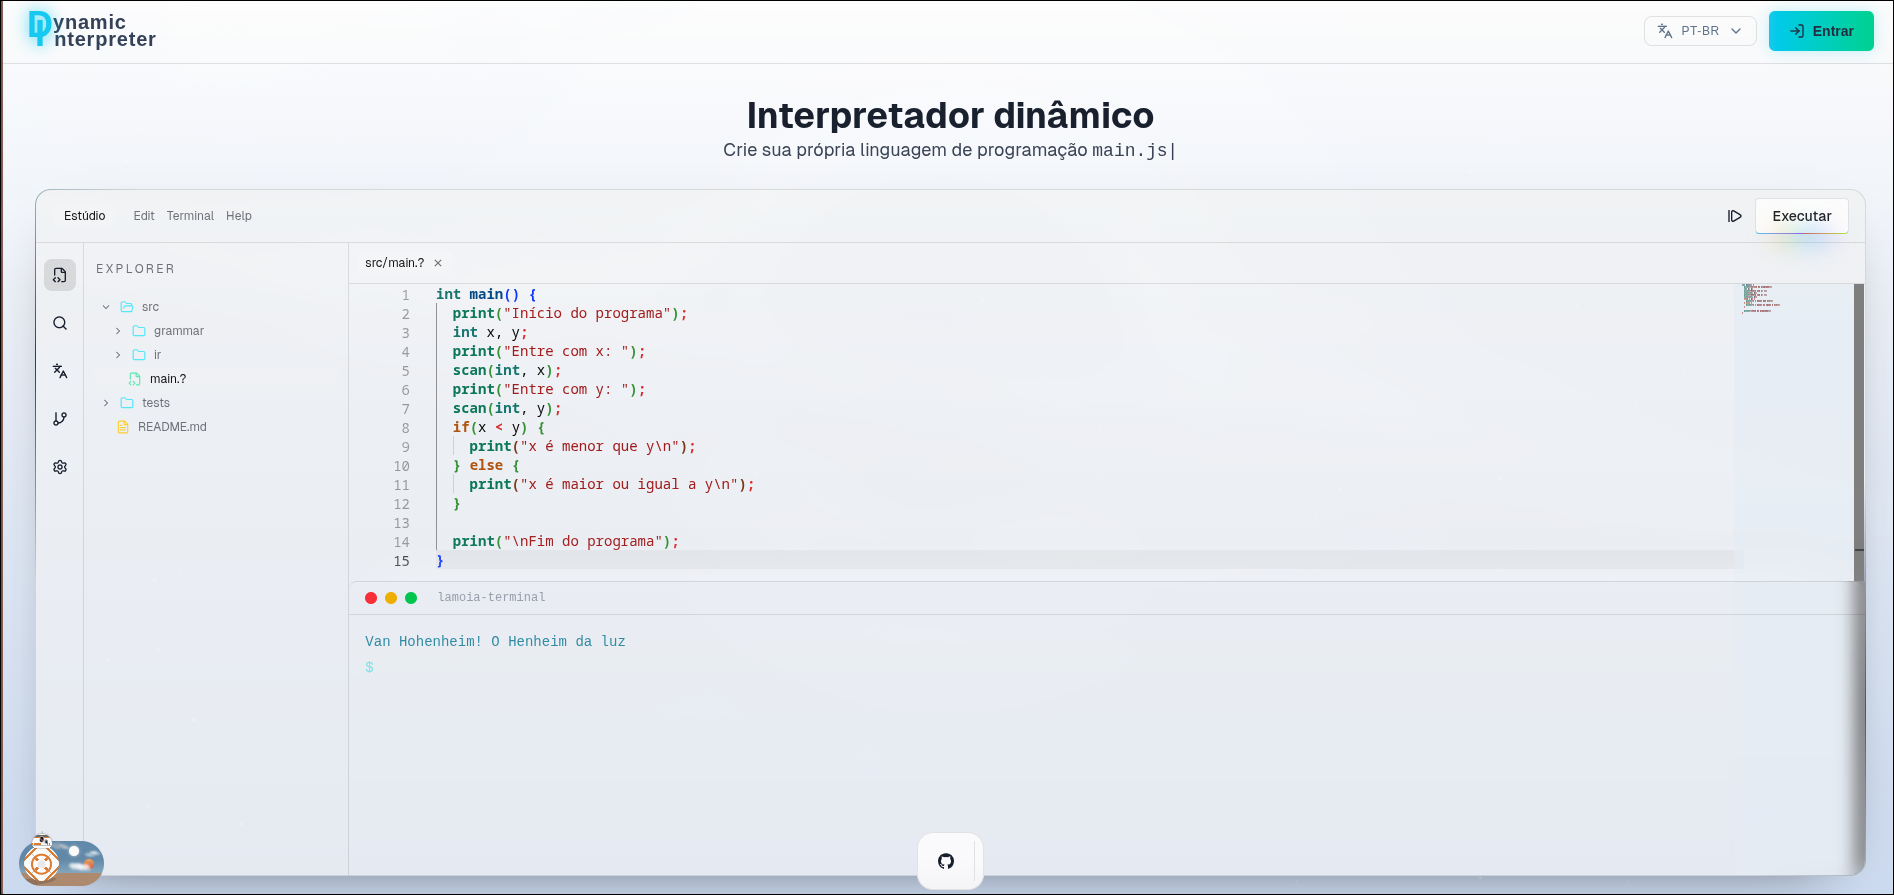
\includegraphics[width=\textwidth]{home_page_light.png}
        \caption{Tema claro.}
        \label{fig:home-light}
    \end{subfigure}

    \vspace{0.8em}

    \begin{subfigure}{0.9\textwidth}
        \centering
        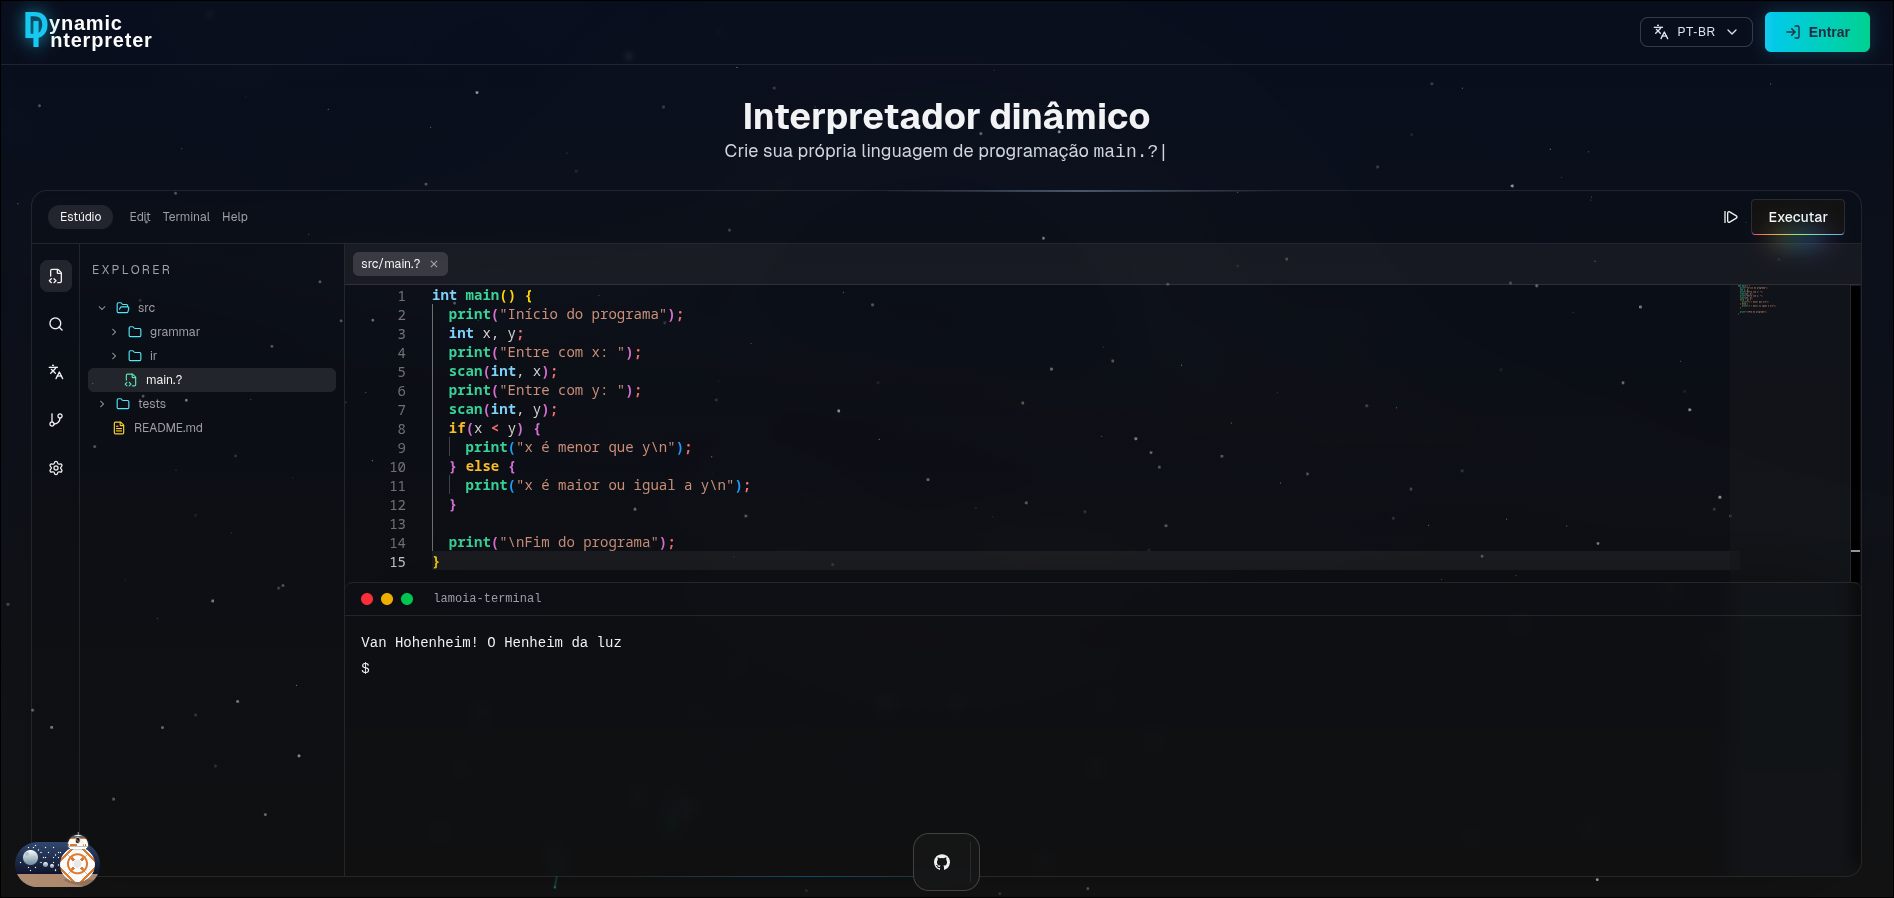
\includegraphics[width=\textwidth]{home_page_dark.png}
        \caption{Tema escuro.}
        \label{fig:home-dark}
    \end{subfigure}
    \caption{Página inicial da plataforma em suas duas variações de tema.}
    \label{fig:home-page}
    \legend{Fonte: elaborado pelo autor.}
\end{figure}

\FloatBarrier

\noindent\textbf{Painel do Aluno}

O painel do aluno consolida, em uma única tela, todas as turmas em que o estudante está matriculado, as listas de exercícios pendentes e o histórico recente de submissões. A tela foi modelada para reduzir o número de cliques necessários até o exercício seguinte, oferecendo cartões interativos que conduzem o aluno diretamente à composição da IDE com a linguagem dinâmica já configurada pelo professor. A Figura~\ref{fig:painel-aluno} ilustra a disposição geral desse painel.

\begin{figure}[H]
    \centering
    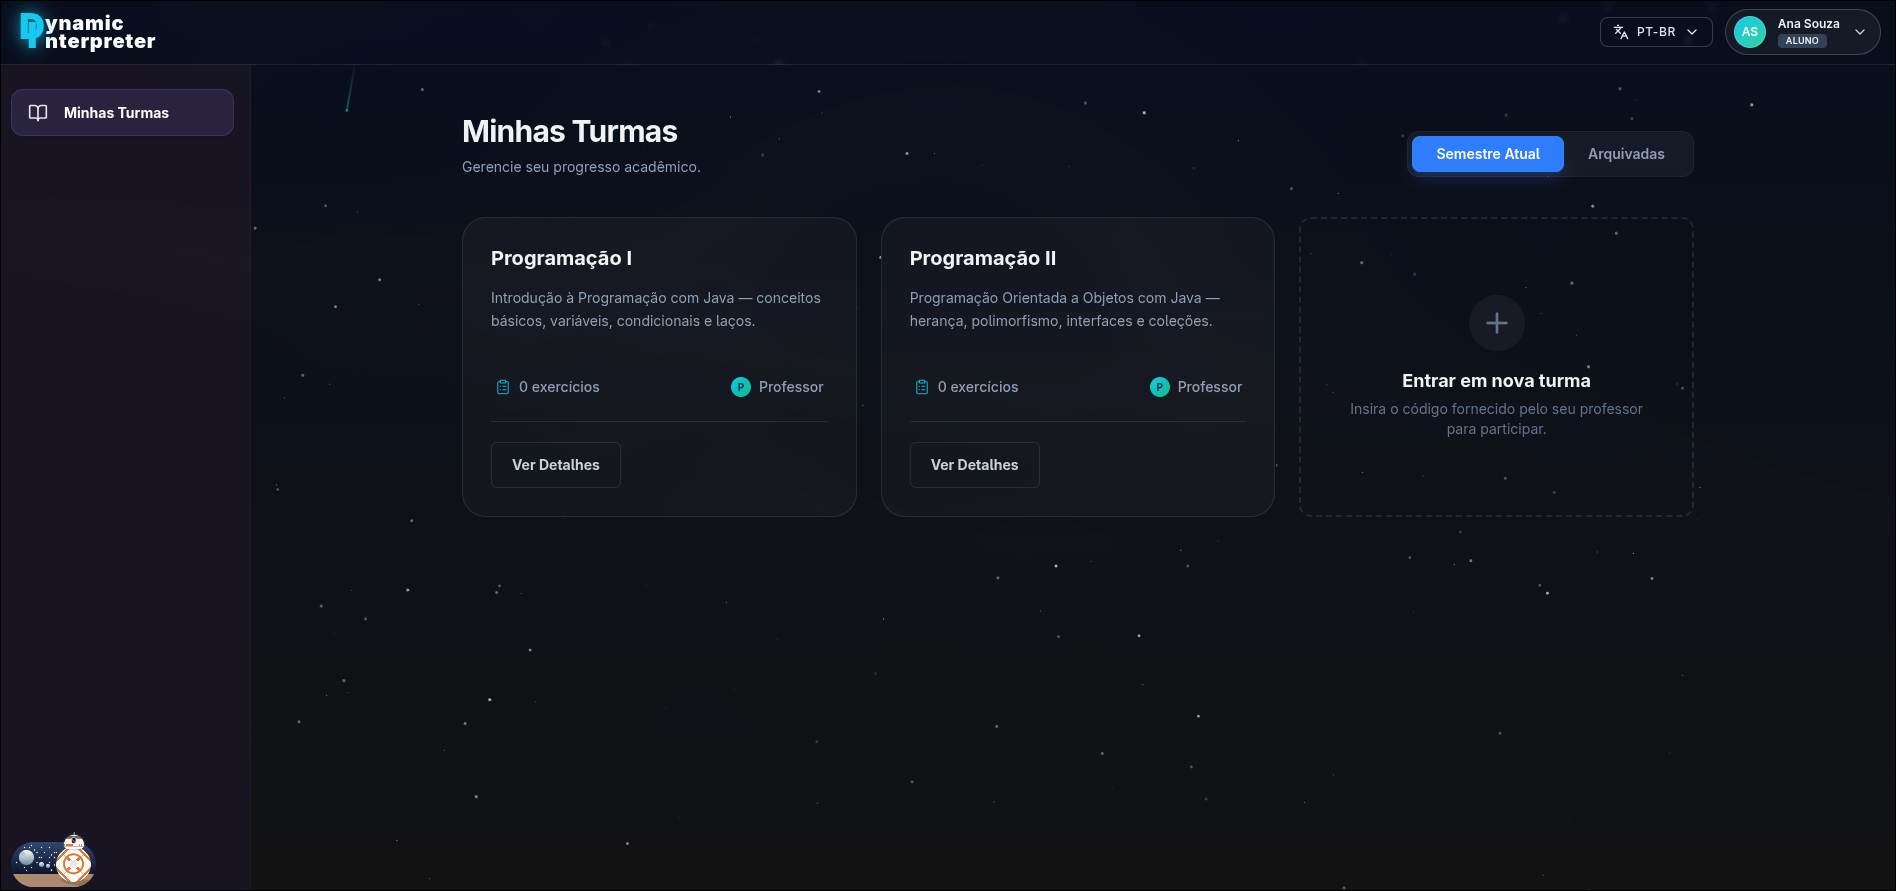
\includegraphics[width=0.85\textwidth]{Aluno/painel_aluno.png}
    \caption{Painel principal do aluno, com acesso às turmas, listas e exercícios.}
    \label{fig:painel-aluno}
    \legend{Fonte: elaborado pelo autor.}
\end{figure}

Ao selecionar uma turma específica, o aluno é conduzido à tela de detalhamento, na qual visualiza informações da disciplina, listas publicadas pelo professor e seu progresso individual em cada exercício. A Figura~\ref{fig:aluno-turma} apresenta essa visão, enquanto a Figura~\ref{fig:aluno-listas} detalha a estrutura interna de uma lista de exercícios, na qual cada item exibe o respectivo estado (não iniciado, em andamento ou submetido) e a configuração da linguagem dinâmica vinculada ao enunciado.

\begin{figure}[h]
    \centering
    \begin{subfigure}{0.9\textwidth}
        \centering
        \includegraphics[width=\textwidth]{Aluno/detail_turma.png}
        \caption{Detalhamento de uma turma do aluno.}
        \label{fig:aluno-turma}
    \end{subfigure}

\end{figure}

\begin{figure}[h]\ContinuedFloat

    \begin{subfigure}{0.9\textwidth}
        \centering
        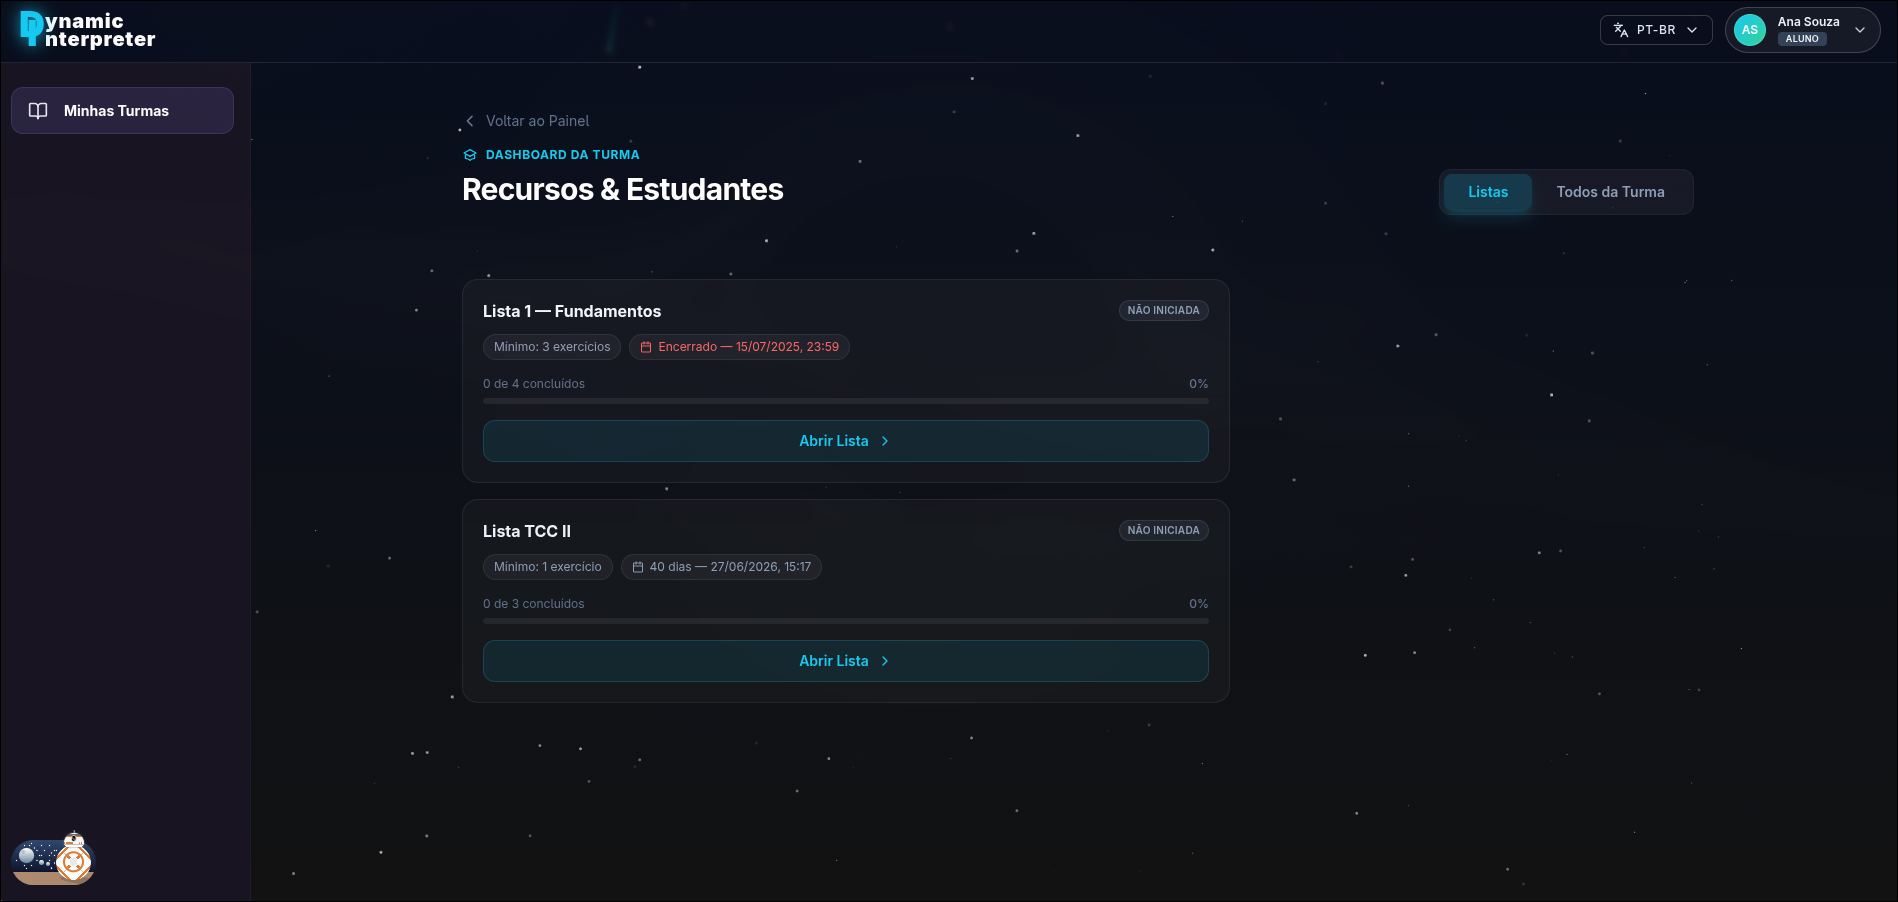
\includegraphics[width=\textwidth]{Aluno/Listas/Listas.png}
        \caption{Lista de exercícios sob a ótica do aluno.}
        \label{fig:aluno-listas}
    \end{subfigure}
    \caption{Composições da experiência do aluno: visão da turma e visão da lista de exercícios.}
    \label{fig:aluno-fluxo}
    \legend{Fonte: elaborado pelo autor.}
\end{figure}

\FloatBarrier

\noindent\textbf{Painel do Professor}

O painel do professor segue a mesma metáfora de organização do painel do aluno, mas amplia o conjunto de ações disponíveis, incorporando criação e gestão de turmas, listas de exercícios e enunciados. A Figura~\ref{fig:painel-professor} apresenta a visão consolidada do professor, com acesso direto às turmas sob sua responsabilidade. Ao selecionar uma turma, são exibidas as listas associadas, conforme a Figura~\ref{fig:professor-turma}, e o conjunto de listas pode ser inspecionado em maior detalhe pela visão dedicada da Figura~\ref{fig:professor-listas-turma}.

\begin{figure}[H]
    \centering
    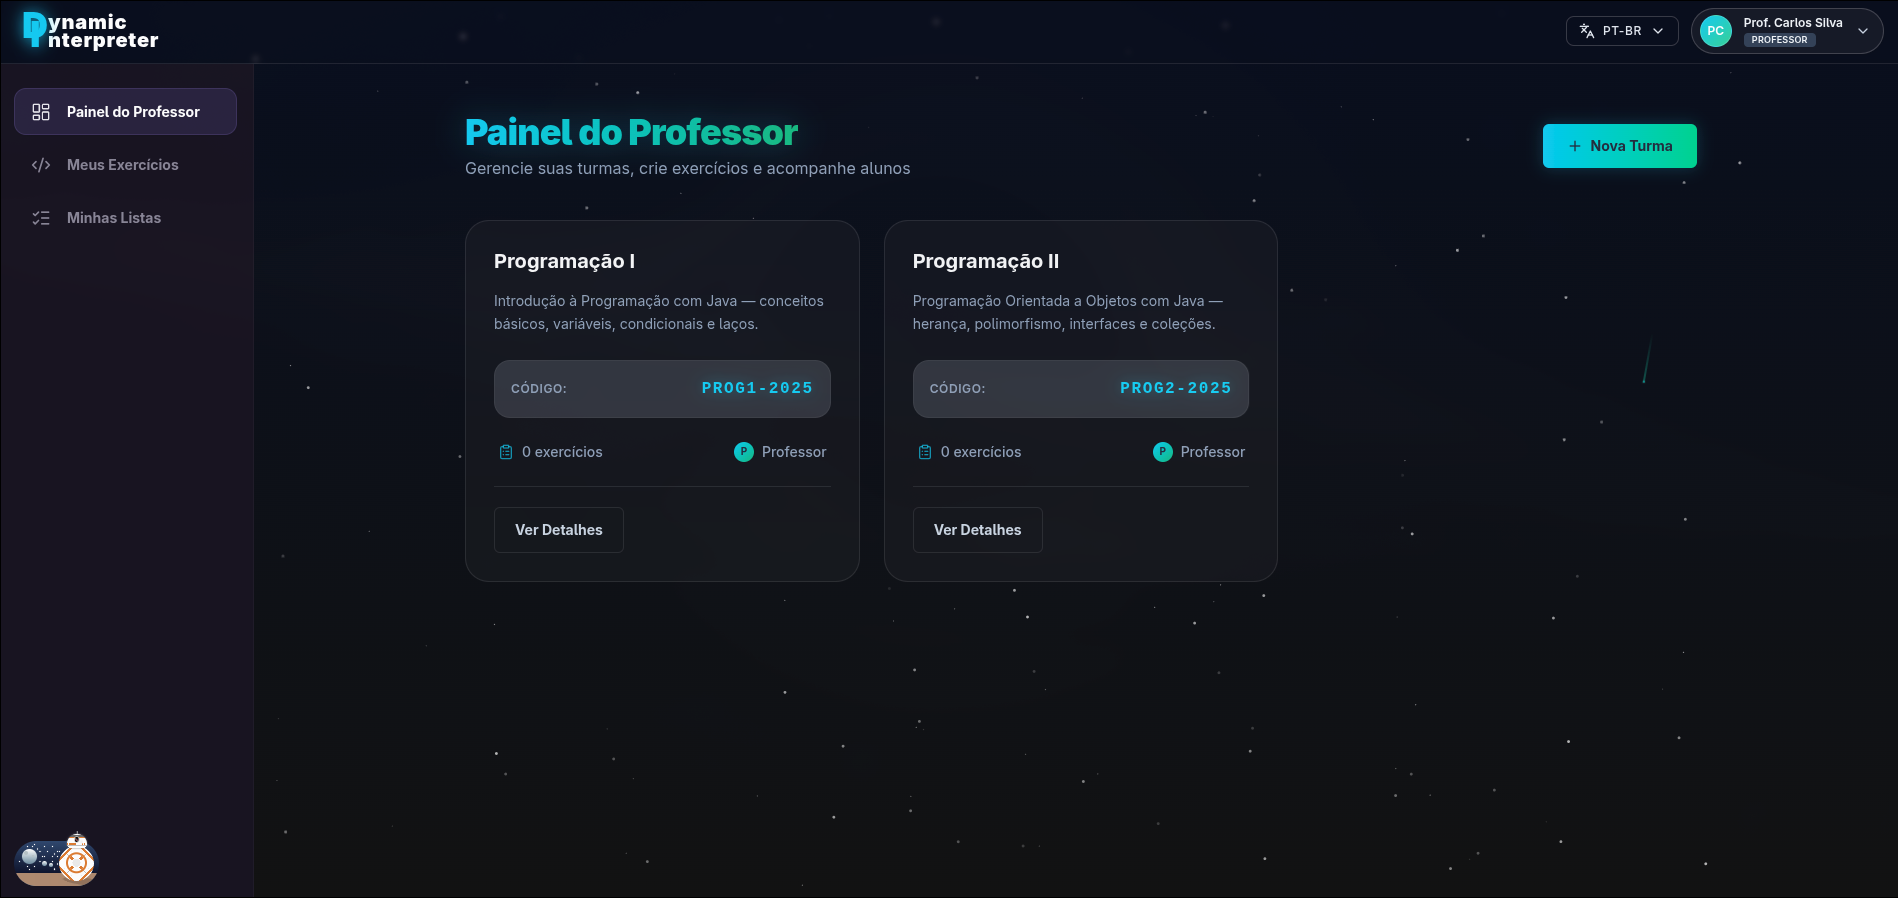
\includegraphics[width=0.85\textwidth]{Professor/painel_professor.png}
    \caption{Painel principal do professor.}
    \label{fig:painel-professor}
    \legend{Fonte: elaborado pelo autor.}
\end{figure}

\begin{figure}[h]
    \centering
    \begin{subfigure}{0.9\textwidth}
        \centering
        \includegraphics[width=\textwidth]{Professor/detail_turma.png}
        \caption{Detalhamento de uma turma do professor.}
        \label{fig:professor-turma}
    \end{subfigure}

\end{figure}

\begin{figure}[h]\ContinuedFloat
\centering
    \begin{subfigure}{0.9\textwidth}
        \centering
        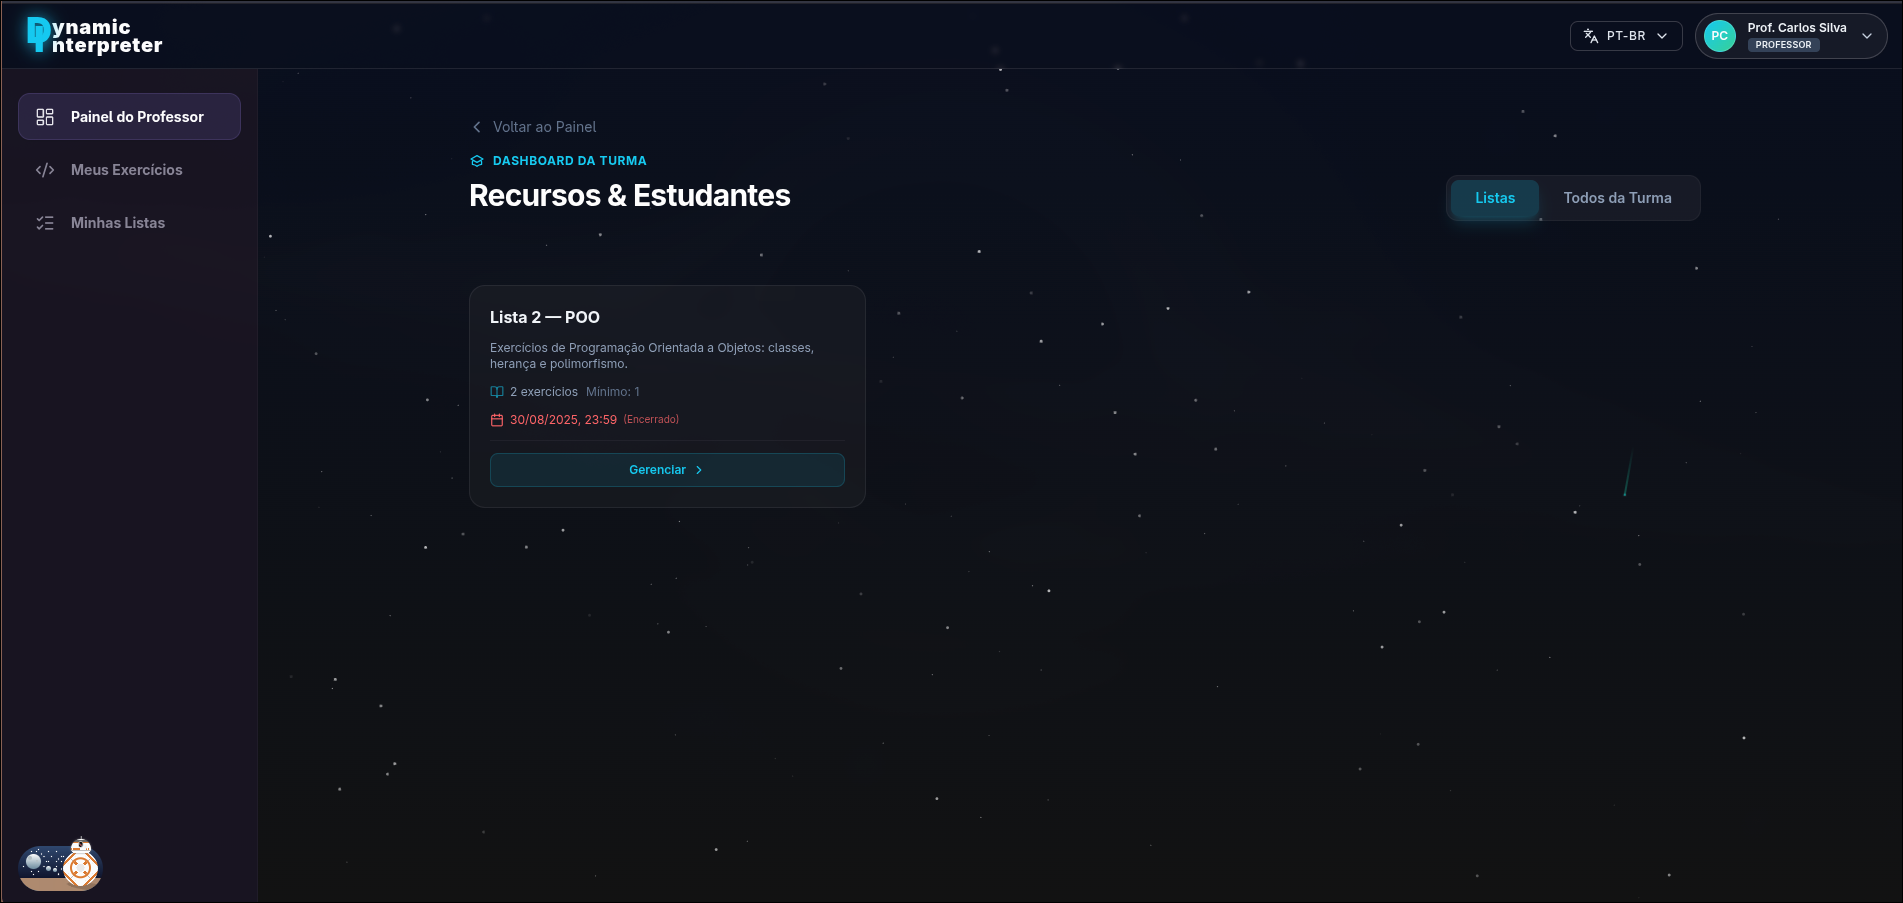
\includegraphics[width=\textwidth]{Professor/listas_turma.png}
        \caption{Listas de exercícios vinculadas à turma.}
        \label{fig:professor-listas-turma}
    \end{subfigure}
    \caption{Composições da experiência do professor: visão da turma e visão das listas associadas.}
    \label{fig:professor-fluxo-turma}
    \legend{Fonte: elaborado pelo autor.}
\end{figure}

\FloatBarrier

\subsubsection*{Gerenciamento de Listas e Exercícios}

A criação e a manutenção de listas pelo professor ocorrem em telas dedicadas que isolam cada operação em um fluxo independente. A Figura~\ref{fig:professor-listas-fluxo} reúne, em uma única composição, as quatro etapas centrais desse processo: a visualização das listas existentes, a configuração dos parâmetros gerais da lista (título, descrição e prazo), a vinculação de exercícios à lista por meio do utilitário de busca e seleção, e a publicação da lista para a turma escolhida.

\begin{figure}[h]
    \centering

    \begin{subfigure}{0.9\textwidth}
        \centering
        
\includegraphics[width=\textwidth]{Professor/Listas/list.png}
        \caption{Listagem das listas existentes.}
        \label{fig:prof-lista-list}
    \end{subfigure}

    \vspace{0.8em}

    \begin{subfigure}{0.9\textwidth}
        \centering
        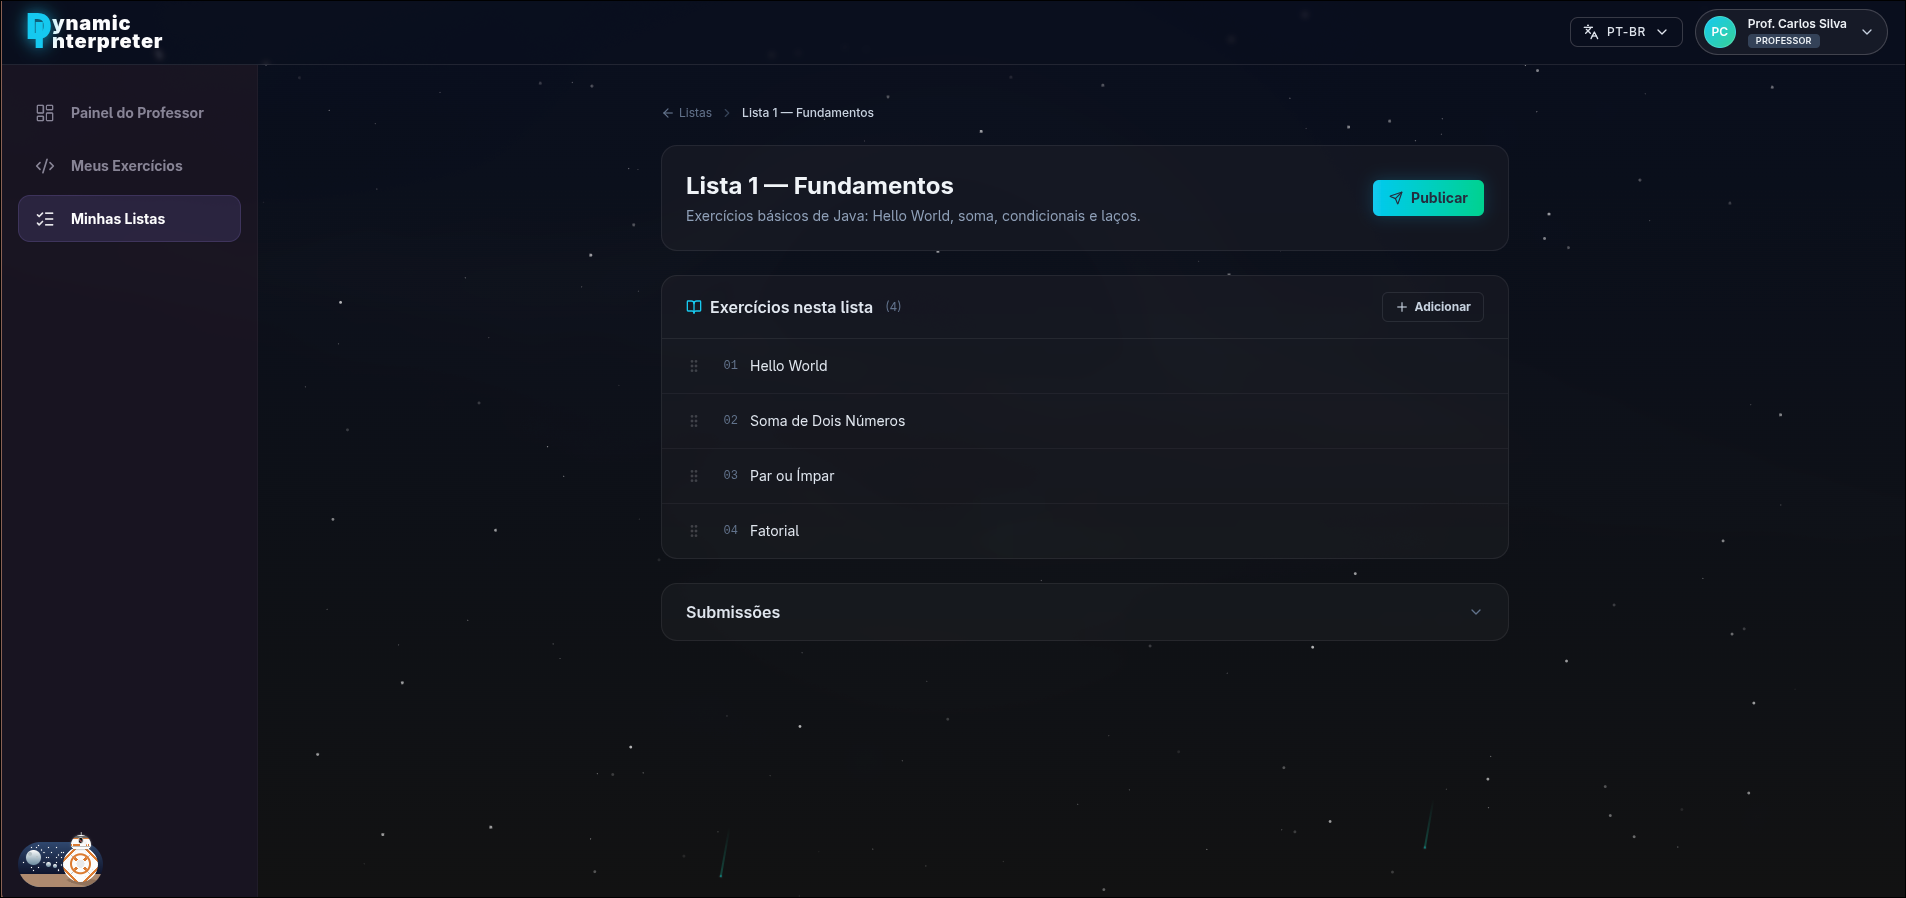
\includegraphics[width=\textwidth]{Professor/Listas/config.png}
        \caption{Configuração dos parâmetros gerais.}
        \label{fig:prof-lista-config}
    \end{subfigure}

\end{figure}

\begin{figure}[p]\ContinuedFloat
    \centering

    \begin{subfigure}{0.9\textwidth}
        \centering
        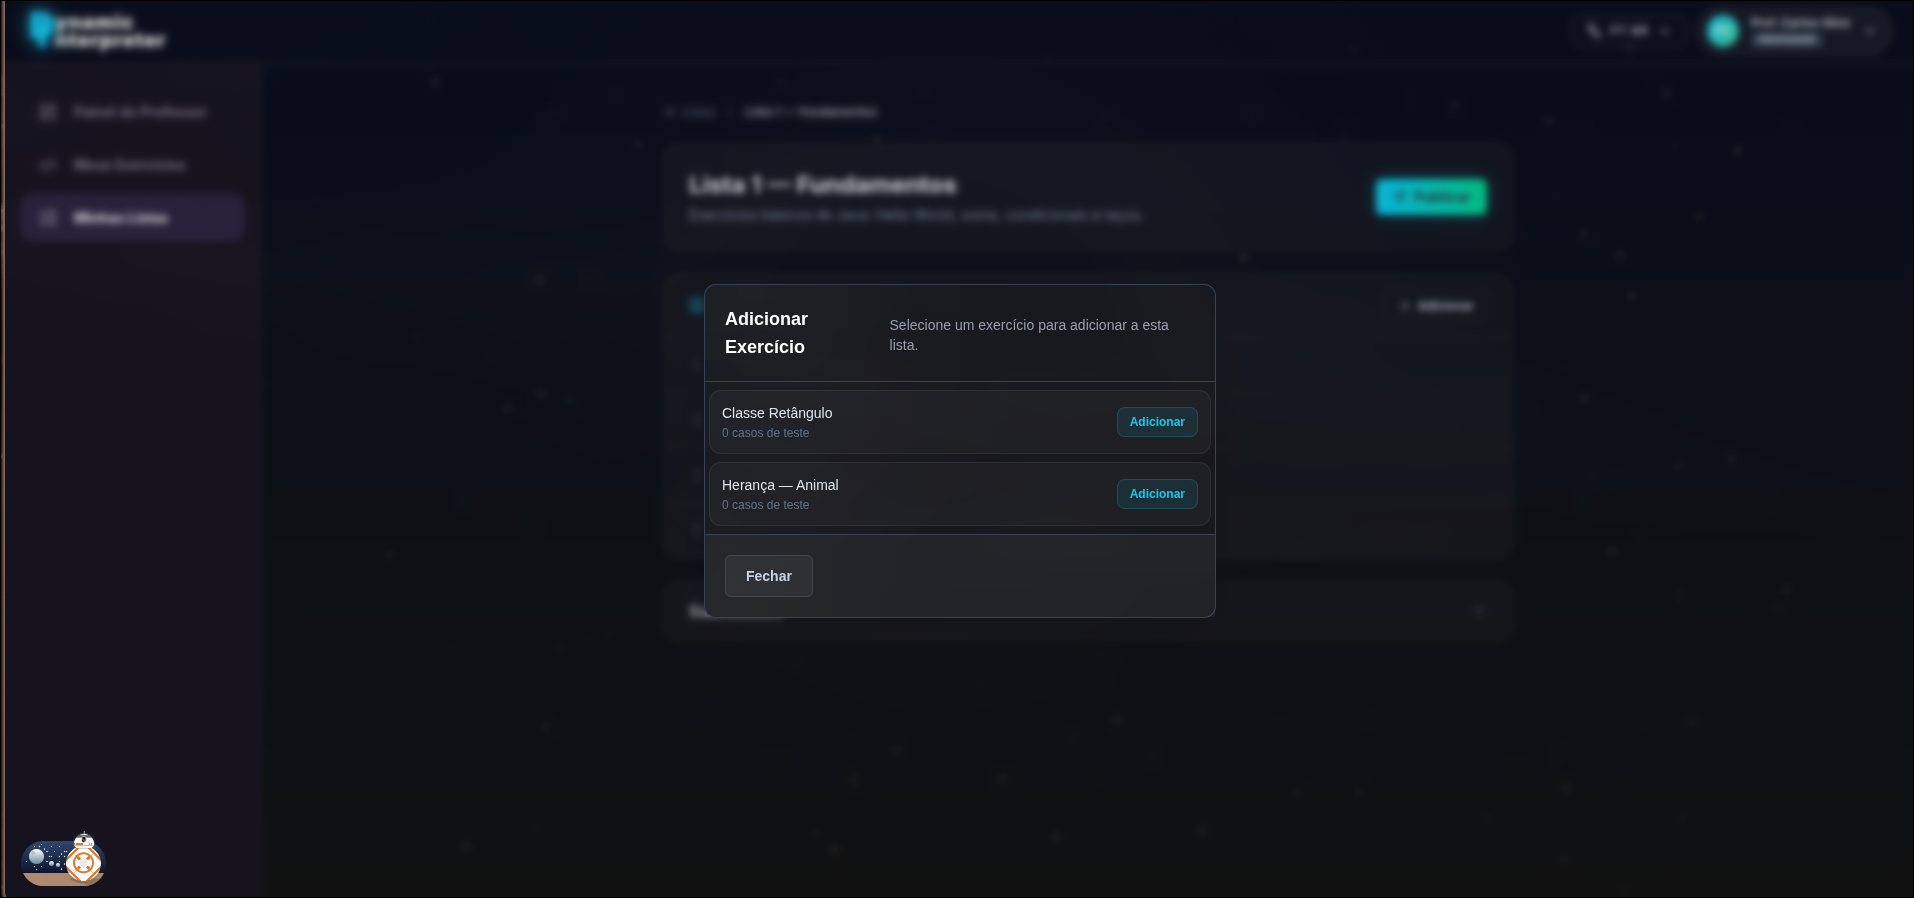
\includegraphics[width=\textwidth]{Professor/Listas/add_exec.png}
        \caption{Vinculação de exercícios à lista.}
        \label{fig:prof-lista-add}
    \end{subfigure}

    \vspace{0.8em}

    \begin{subfigure}{0.9\textwidth}
        \centering
        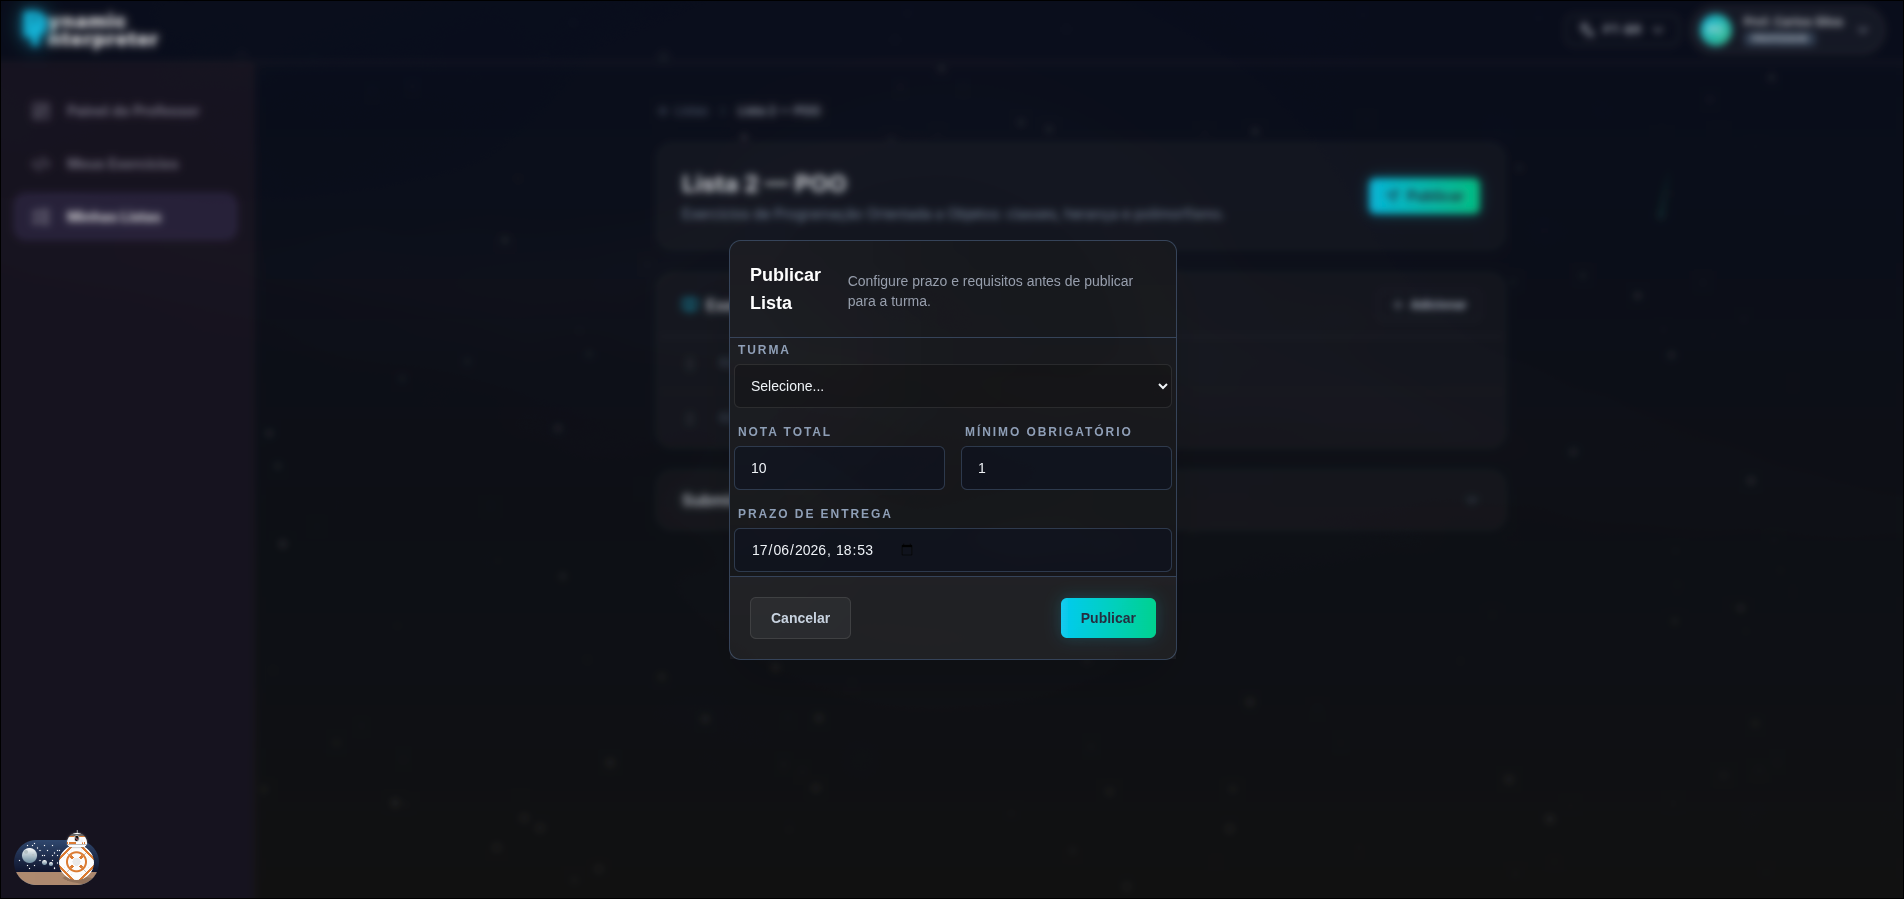
\includegraphics[width=\textwidth]{Professor/Listas/publish.png}
        \caption{Publicação da lista para a turma.}
        \label{fig:prof-lista-publish}
    \end{subfigure}

    \caption{Fluxo de criação e gestão de listas de exercícios pelo professor.}
    \label{fig:professor-listas-fluxo}
    \legend{Fonte: elaborado pelo autor.}
\end{figure}

\FloatBarrier

A gestão dos enunciados individuais ocorre em um conjunto análogo de telas, ilustrado pela Figura~\ref{fig:professor-exercicios-fluxo}. A tela de listagem permite a busca, a filtragem e a ordenação dos enunciados; a tela de criação centraliza, em um único formulário, a descrição do problema, os casos de teste com entradas e saídas esperadas e a vinculação a uma imagem de linguagem que delimita o vocabulário disponível ao aluno; a tela de detalhamento mostra a composição final do exercício; e a tela de submissões consolida todas as resoluções enviadas pelos alunos, com os respectivos vereditos do subsistema de avaliação automatizada discutido na Seção~\ref{sec:sistema-correcao}.

\begin{figure}[h]
    \centering
    \begin{subfigure}{0.9\textwidth}
        \centering
        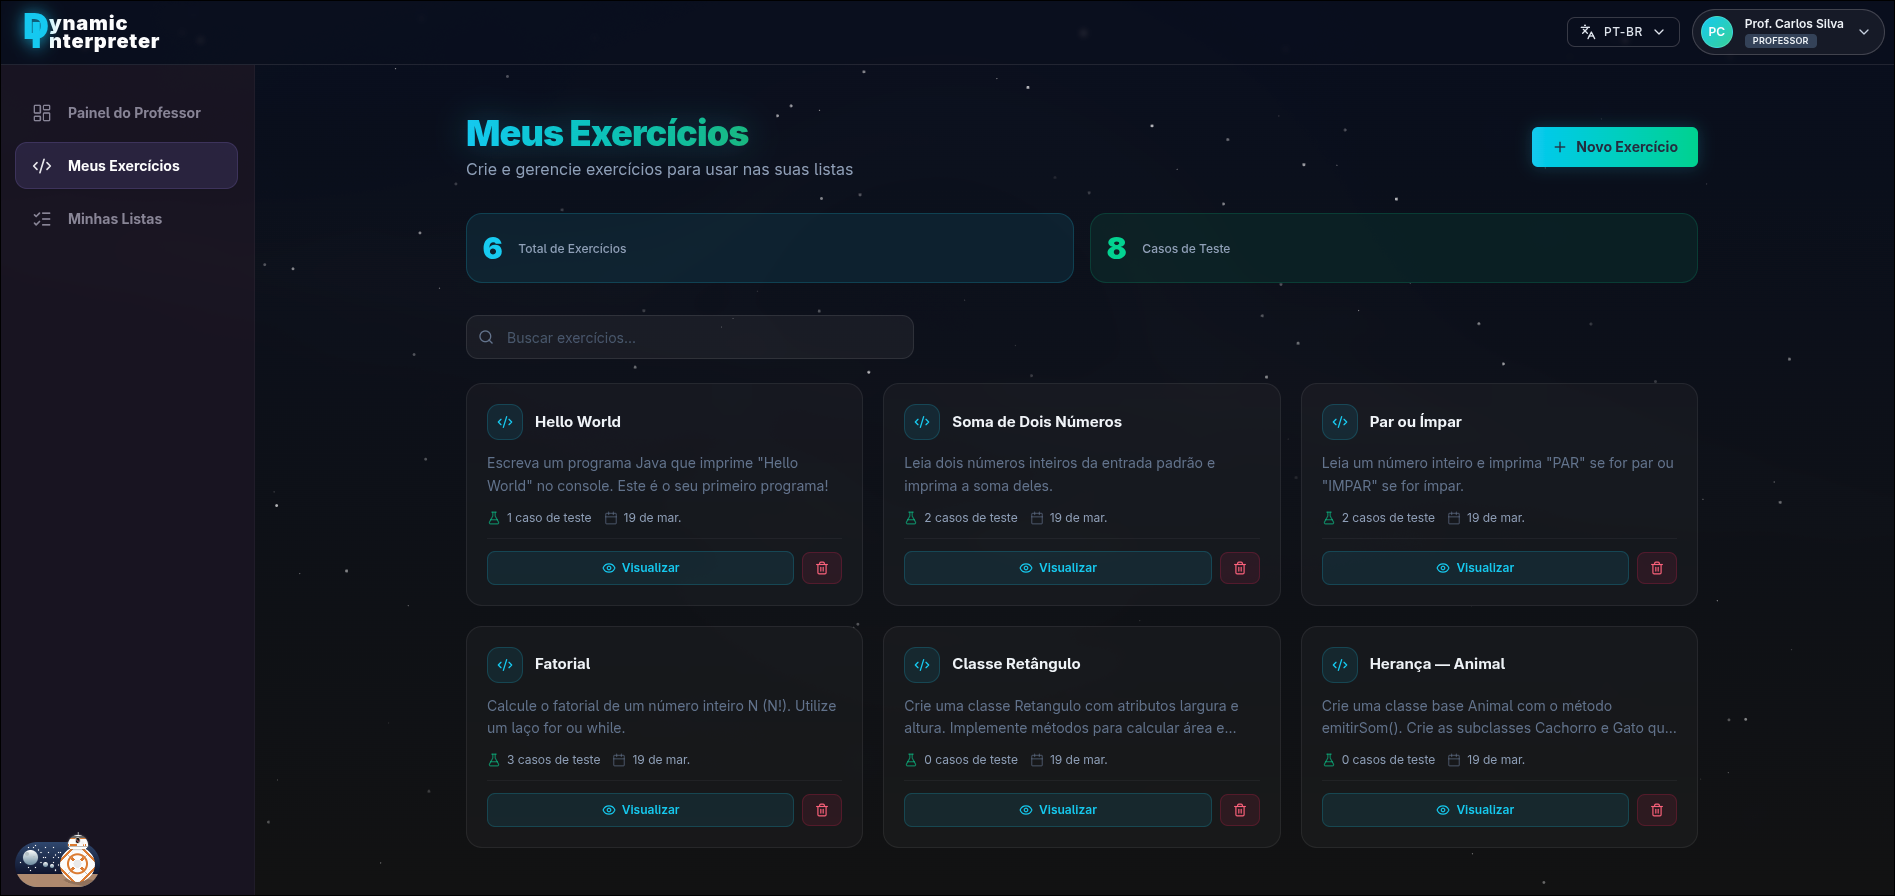
\includegraphics[width=\textwidth]{Professor/Exercicios/list.png}
        \caption{Listagem dos enunciados existentes.}
        \label{fig:prof-exec-list}
    \end{subfigure}

    \vspace{0.8em}

    \begin{subfigure}{0.9\textwidth}
        \centering
        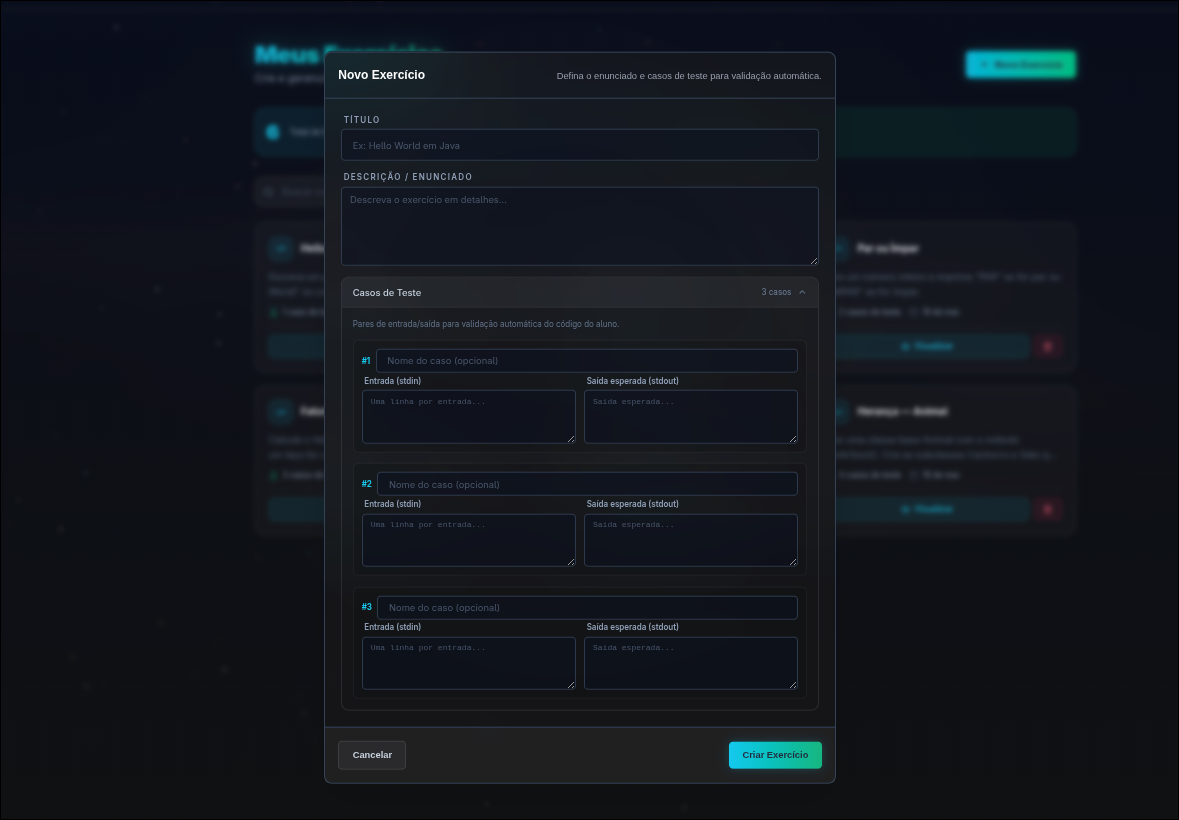
\includegraphics[width=\textwidth]{Professor/Exercicios/create.png}
        \caption{Criação de um novo enunciado.}
        \label{fig:prof-exec-create}
    \end{subfigure}

\end{figure}

\begin{figure}[p]\ContinuedFloat
    \centering

    \begin{subfigure}{0.9\textwidth}
        \centering
        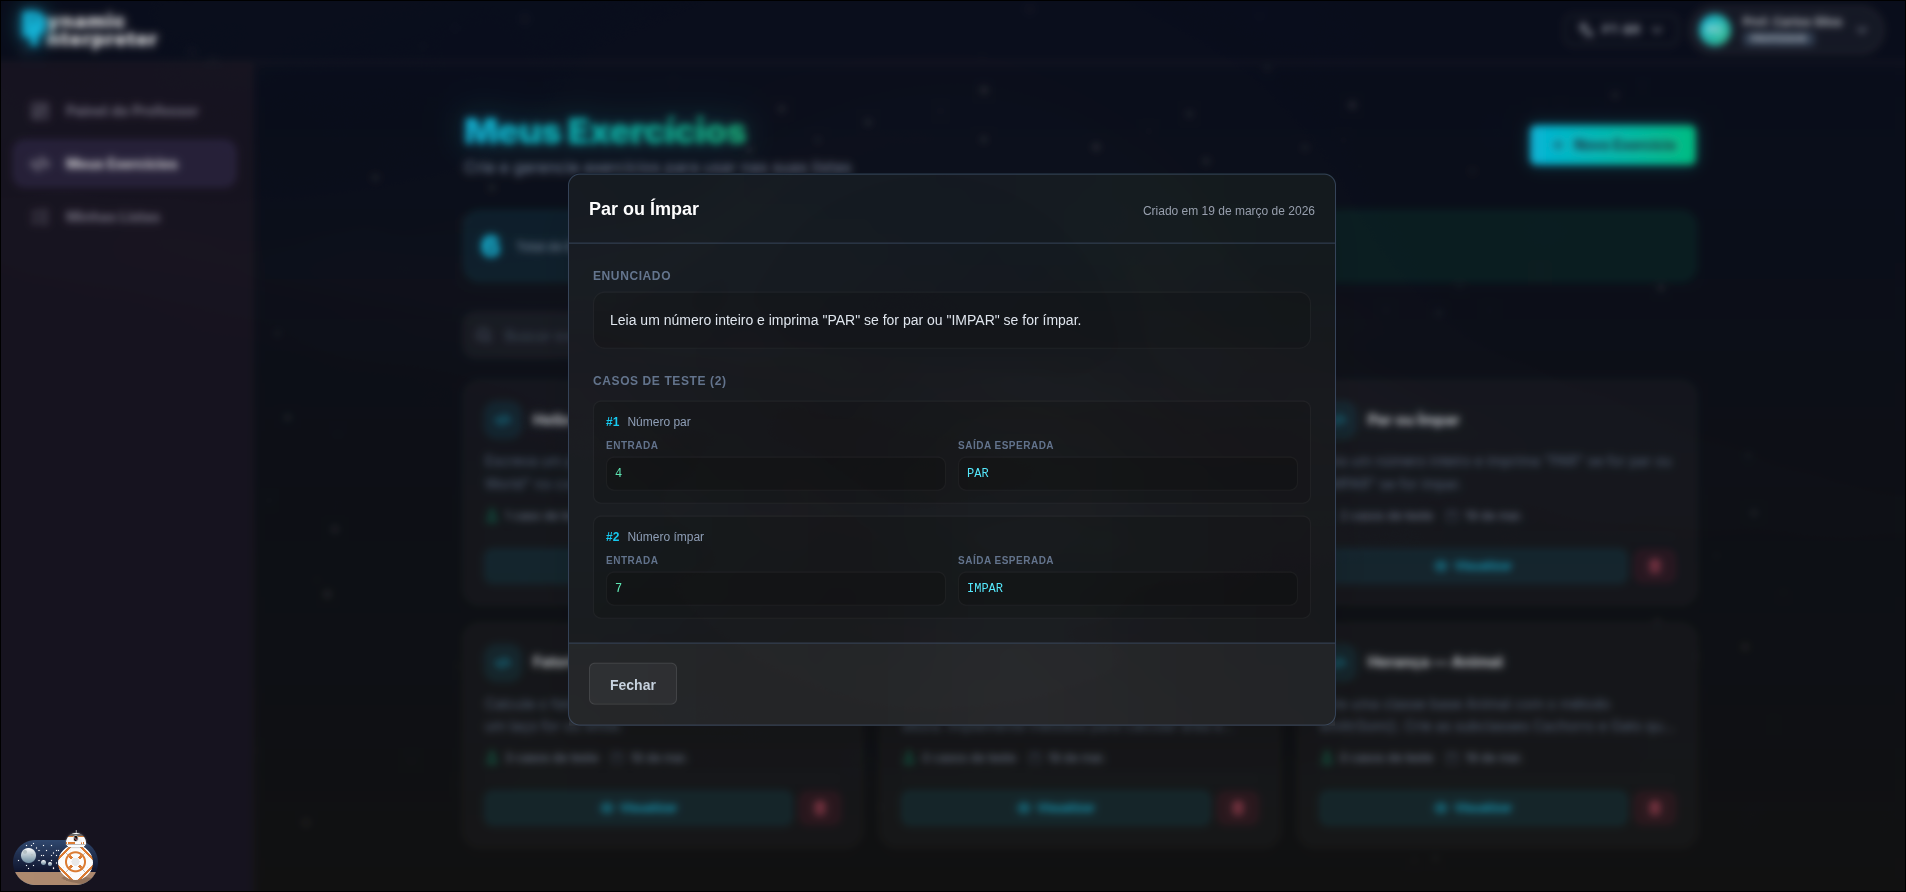
\includegraphics[width=\textwidth]{Professor/Exercicios/detail.png}
        \caption{Detalhamento de um exercício.}
        \label{fig:prof-exec-detail}
    \end{subfigure}

    \vspace{0.8em}

    \begin{subfigure}{0.9\textwidth}
        \centering
        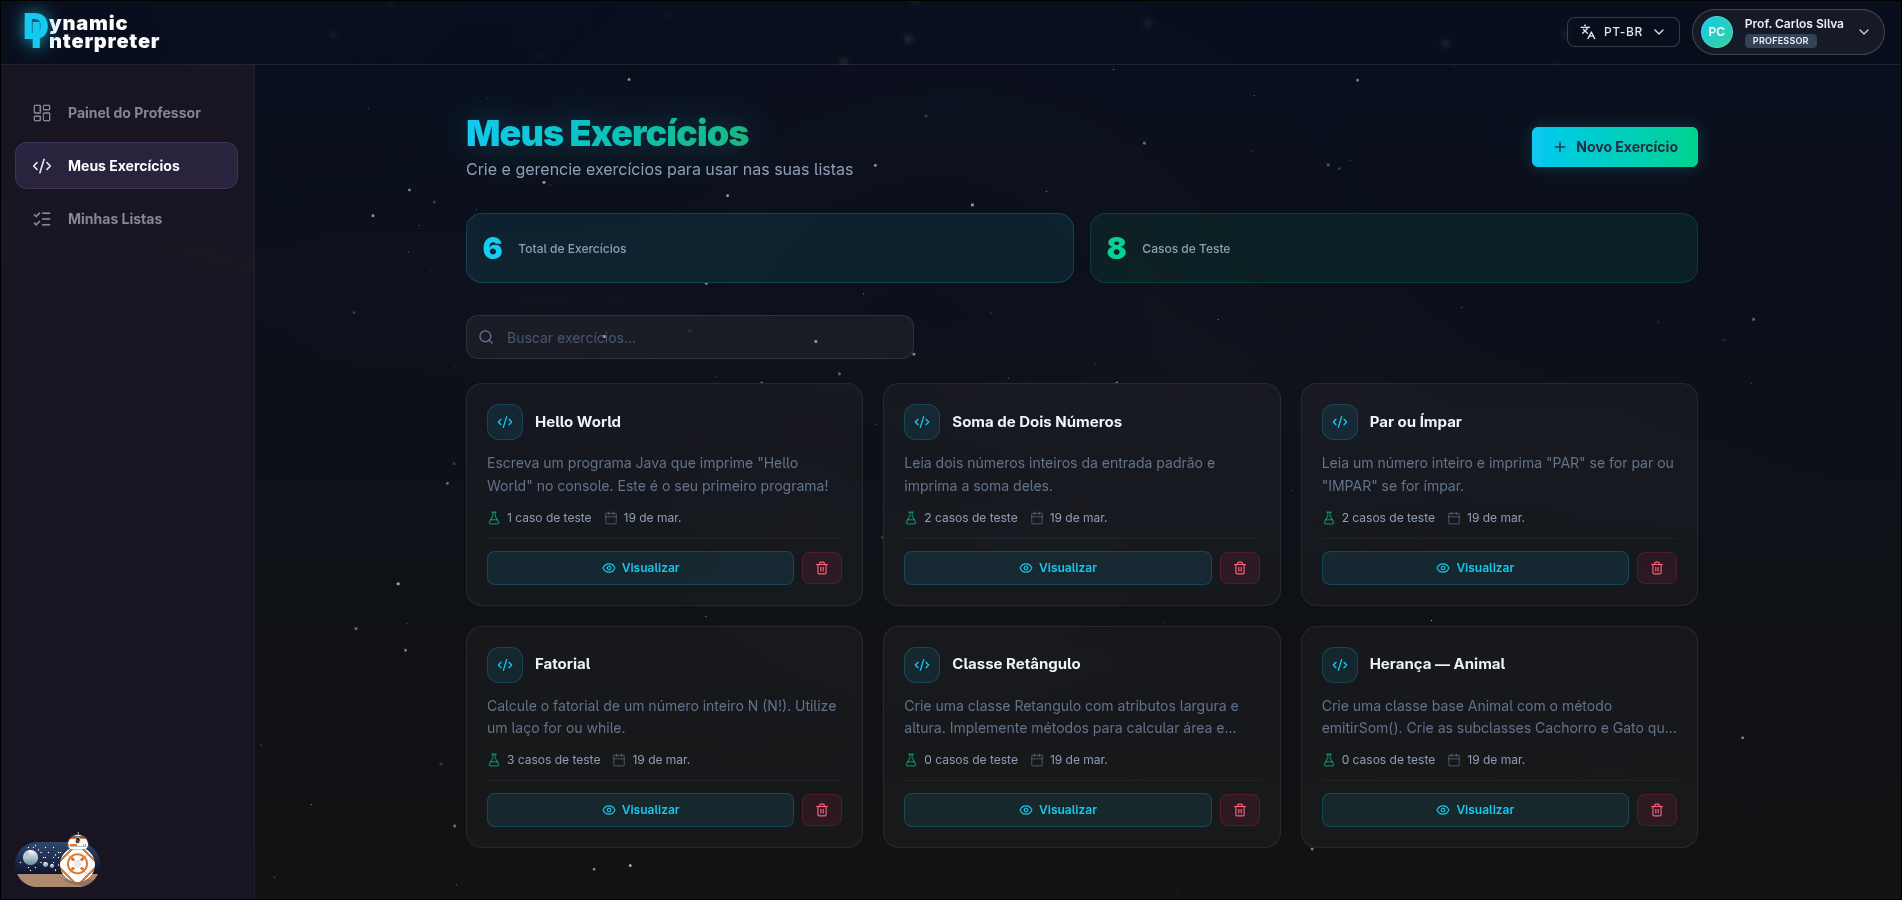
\includegraphics[width=\textwidth]{Professor/Exercicios/execs.png}
        \caption{Submissões dos alunos para o exercício.}
        \label{fig:prof-exec-execs}
    \end{subfigure}
    \caption{Fluxo de criação e acompanhamento dos enunciados pelo professor.}
    \label{fig:professor-exercicios-fluxo}
    \legend{Fonte: elaborado pelo autor.}
\end{figure}

\FloatBarrier

\subsection{Fluxo de Personalização da Linguagem Dinâmica}

A funcionalidade central da plataforma, que corresponde à personalização dinâmica do vocabulário e das regras estruturais da linguagem, foi materializada em um assistente progressivo composto por seis etapas sequenciais. Esse \textit{wizard}, discutido na Seção~\ref{sec:customizacao-dinamica}, conduz o usuário por escolhas independentes, validadas isoladamente, com geração de \textit{preview} em tempo real do código resultante. As figuras a seguir documentam, em ordem, cada uma das etapas efetivamente implementadas.

\begin{figure}[h]
    \centering
    \begin{subfigure}{0.9\textwidth}
        \centering
        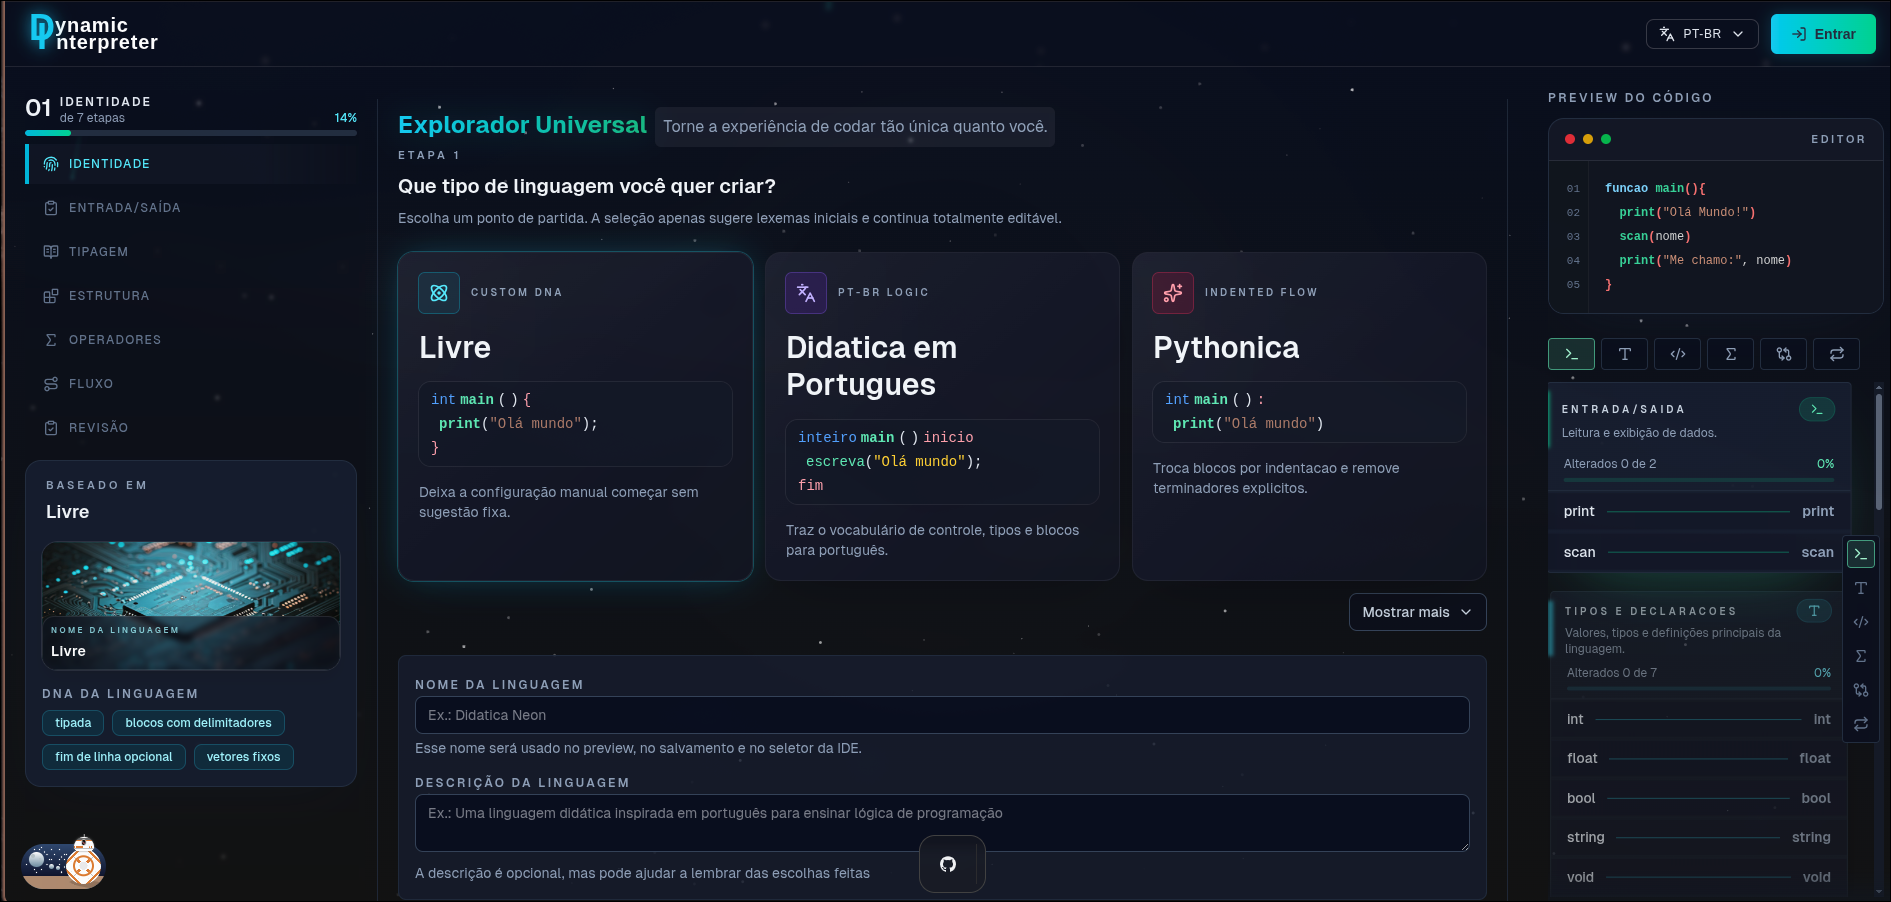
\includegraphics[width=\textwidth]{Etapas/etapa1.png}
        \caption{Etapa 1: definição do nome da linguagem e da identidade da customização.}
        \label{fig:etapa1}
    \end{subfigure}

    \vspace{0.8em}

    \begin{subfigure}{0.9\textwidth}
        \centering
        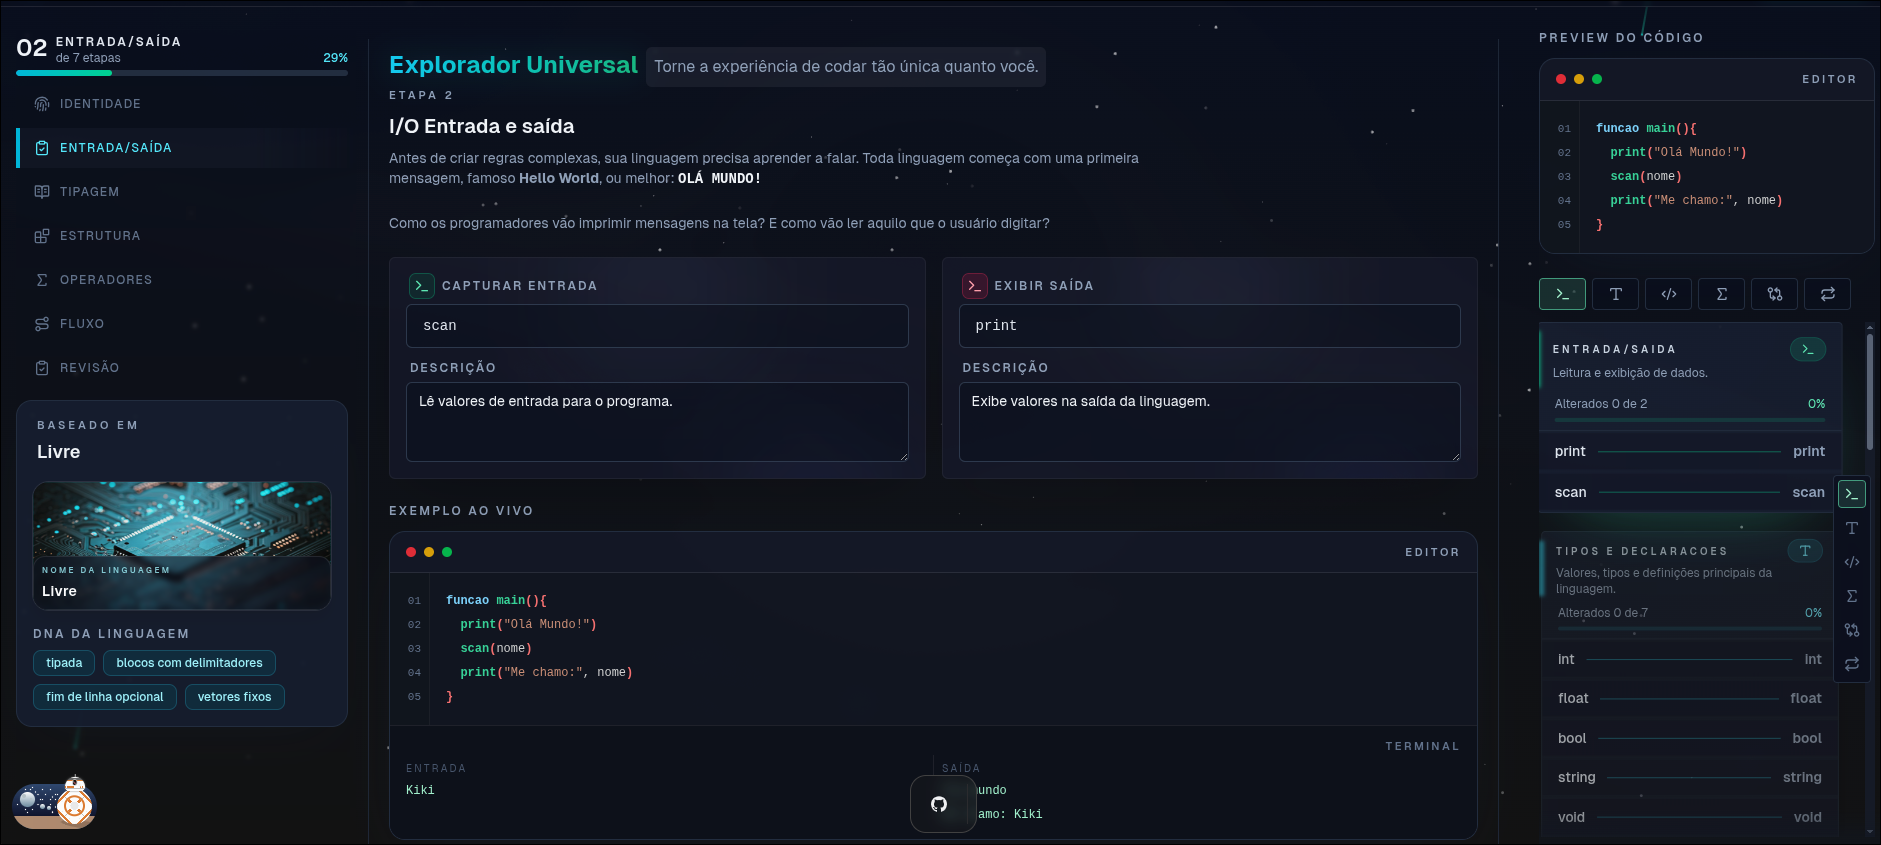
\includegraphics[width=\textwidth]{Etapas/etapa2.png}
        \caption{Etapa 2: configuração das palavras-chave de tipos primitivos.}
        \label{fig:etapa2}
    \end{subfigure}
      \caption{Etapas 1 e 2 do assistente de personalização da linguagem dinâmica.}
      \label{fig:etapas-1-2}
      \legend{Fonte: elaborado pelo autor.}
\end{figure}

\FloatBarrier

A terceira etapa concentra-se na personalização das palavras-chave de controle de fluxo, oferecendo ao usuário a possibilidade de redefinir comandos como \texttt{if}, \texttt{else}, \texttt{for}, \texttt{while}, \texttt{break}, \texttt{continue} e \texttt{return}. A Figura~\ref{fig:etapas-3} apresenta as duas variações dessa etapa, contemplando a configuração das palavras-chave básicas e a configuração estendida com construtores como \texttt{switch} e \texttt{case}.

\begin{figure}[h]
    \centering
    \begin{subfigure}{0.9\textwidth}
        \centering
        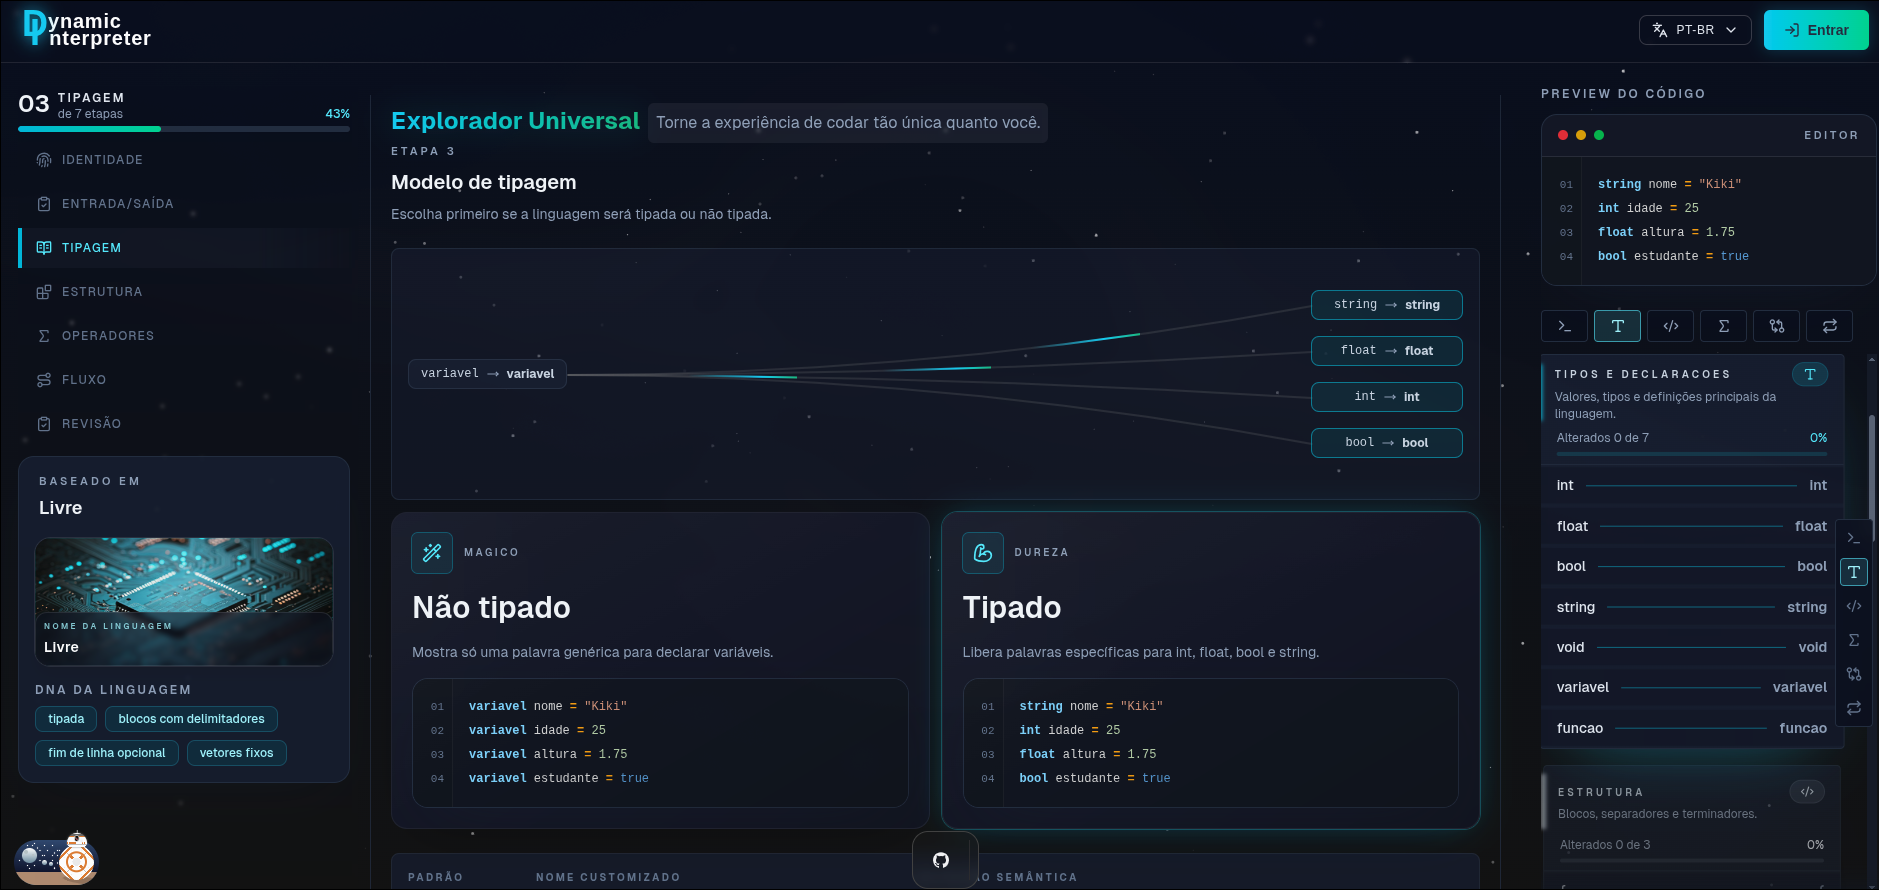
\includegraphics[width=\textwidth]{Etapas/etapa3_1.png}
        \caption{Etapa 3.1: palavras-chave básicas de controle de fluxo.}
        \label{fig:etapa3-1}
    \end{subfigure}

    \vspace{0.8em}

    \begin{subfigure}{0.9\textwidth}
        \centering
        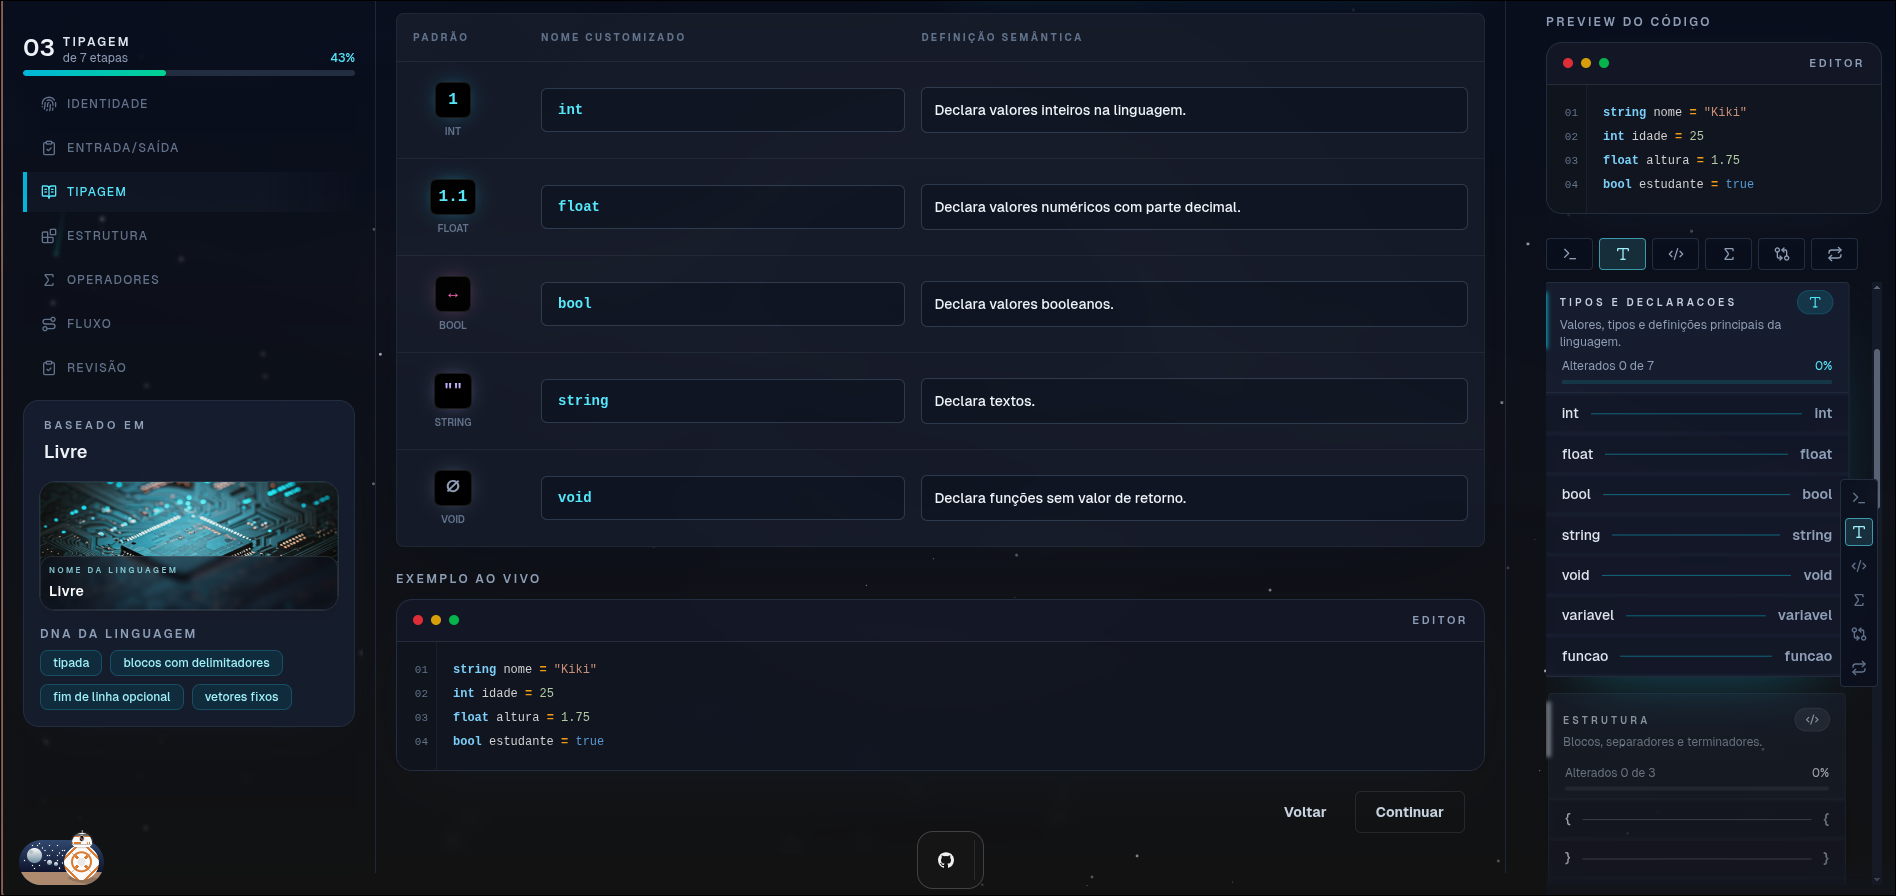
\includegraphics[width=\textwidth]{Etapas/etapa3_2.png}
        \caption{Etapa 3.2: construtores estendidos de controle de fluxo.}
        \label{fig:etapa3-2}
    \end{subfigure}
    \caption{Etapa 3 do assistente, dedicada às palavras-chave de controle de fluxo.}
    \label{fig:etapas-3}
    \legend{Fonte: elaborado pelo autor.}
\end{figure}

\FloatBarrier

A quarta etapa habilita a substituição de operadores lógicos e relacionais por palavras de uso natural, em consonância com os achados empíricos de \citeonline{stefik2013} sobre o impacto de símbolos obscuros na carga cognitiva inicial. A Figura~\ref{fig:etapas-4} ilustra as duas variações dessa etapa, contemplando, primeiro, a definição de operadores lógicos como \texttt{e}, \texttt{ou} e \texttt{não} e, em seguida, a redefinição dos operadores relacionais por meio do mesmo princípio de palavras significativas.

\begin{figure}[p]
    \centering
    \begin{subfigure}{0.9\textwidth}
        \centering
        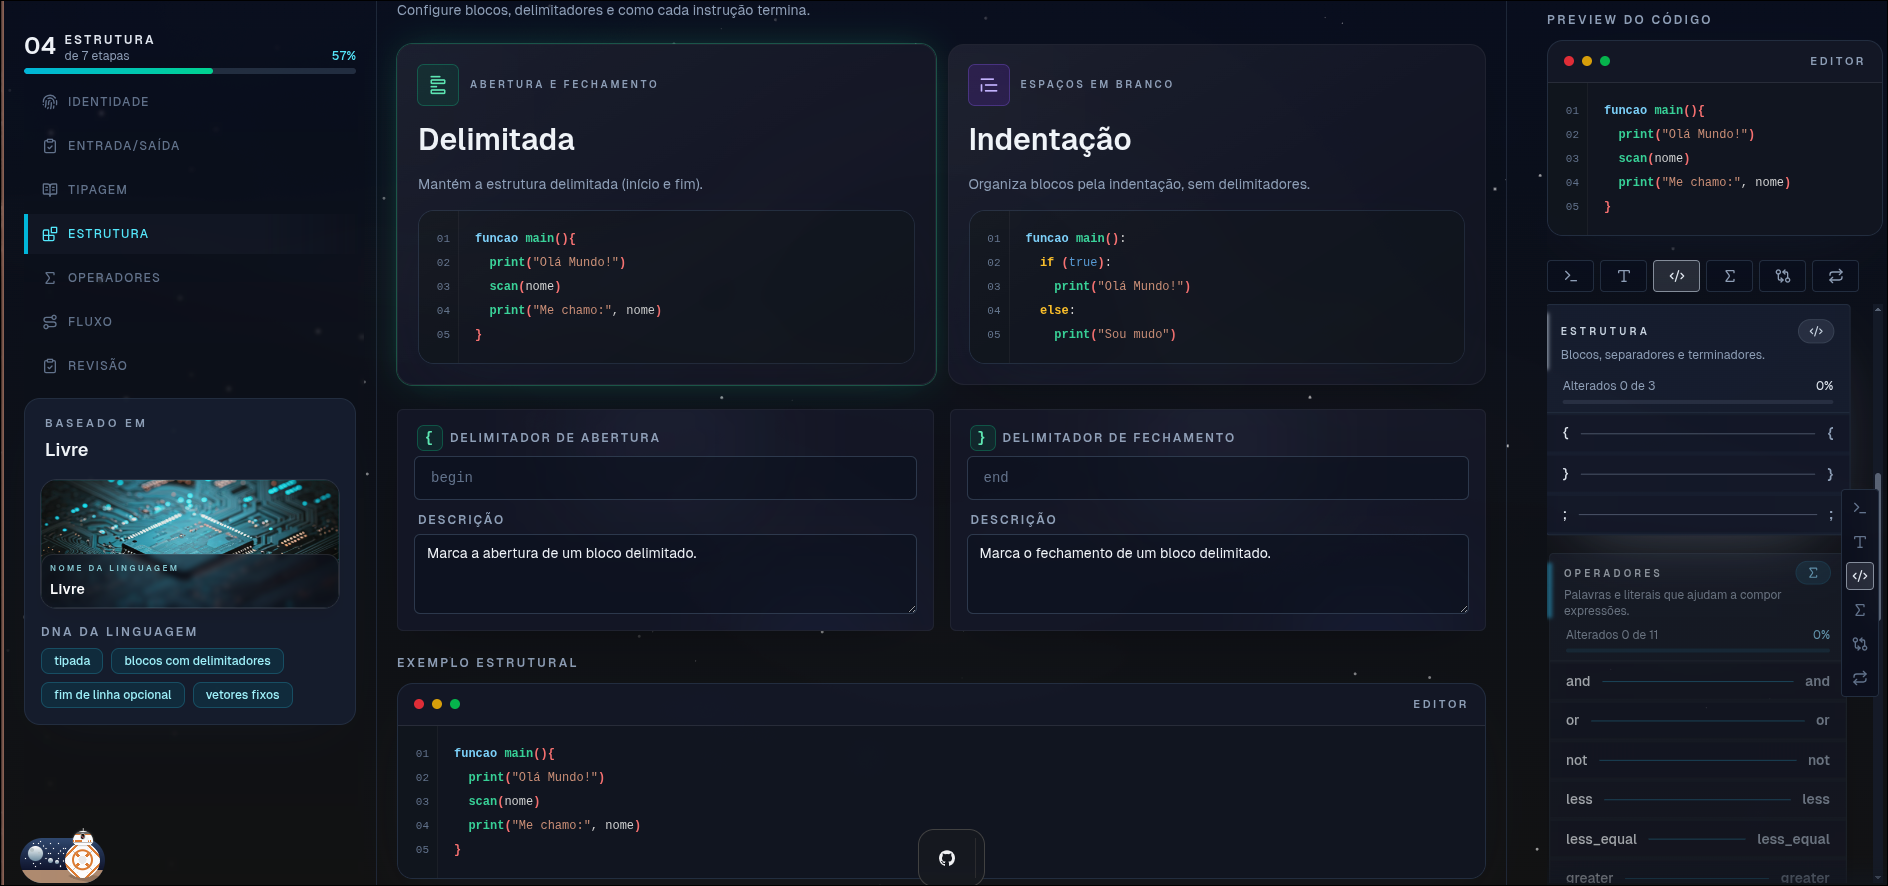
\includegraphics[width=\textwidth]{Etapas/etapa4_1.png}
        \caption{Etapa 4.1: operadores lógicos em forma de palavra.}
        \label{fig:etapa4-1}
    \end{subfigure}

    \vspace{0.8em}

    \begin{subfigure}{0.9\textwidth}
        \centering
        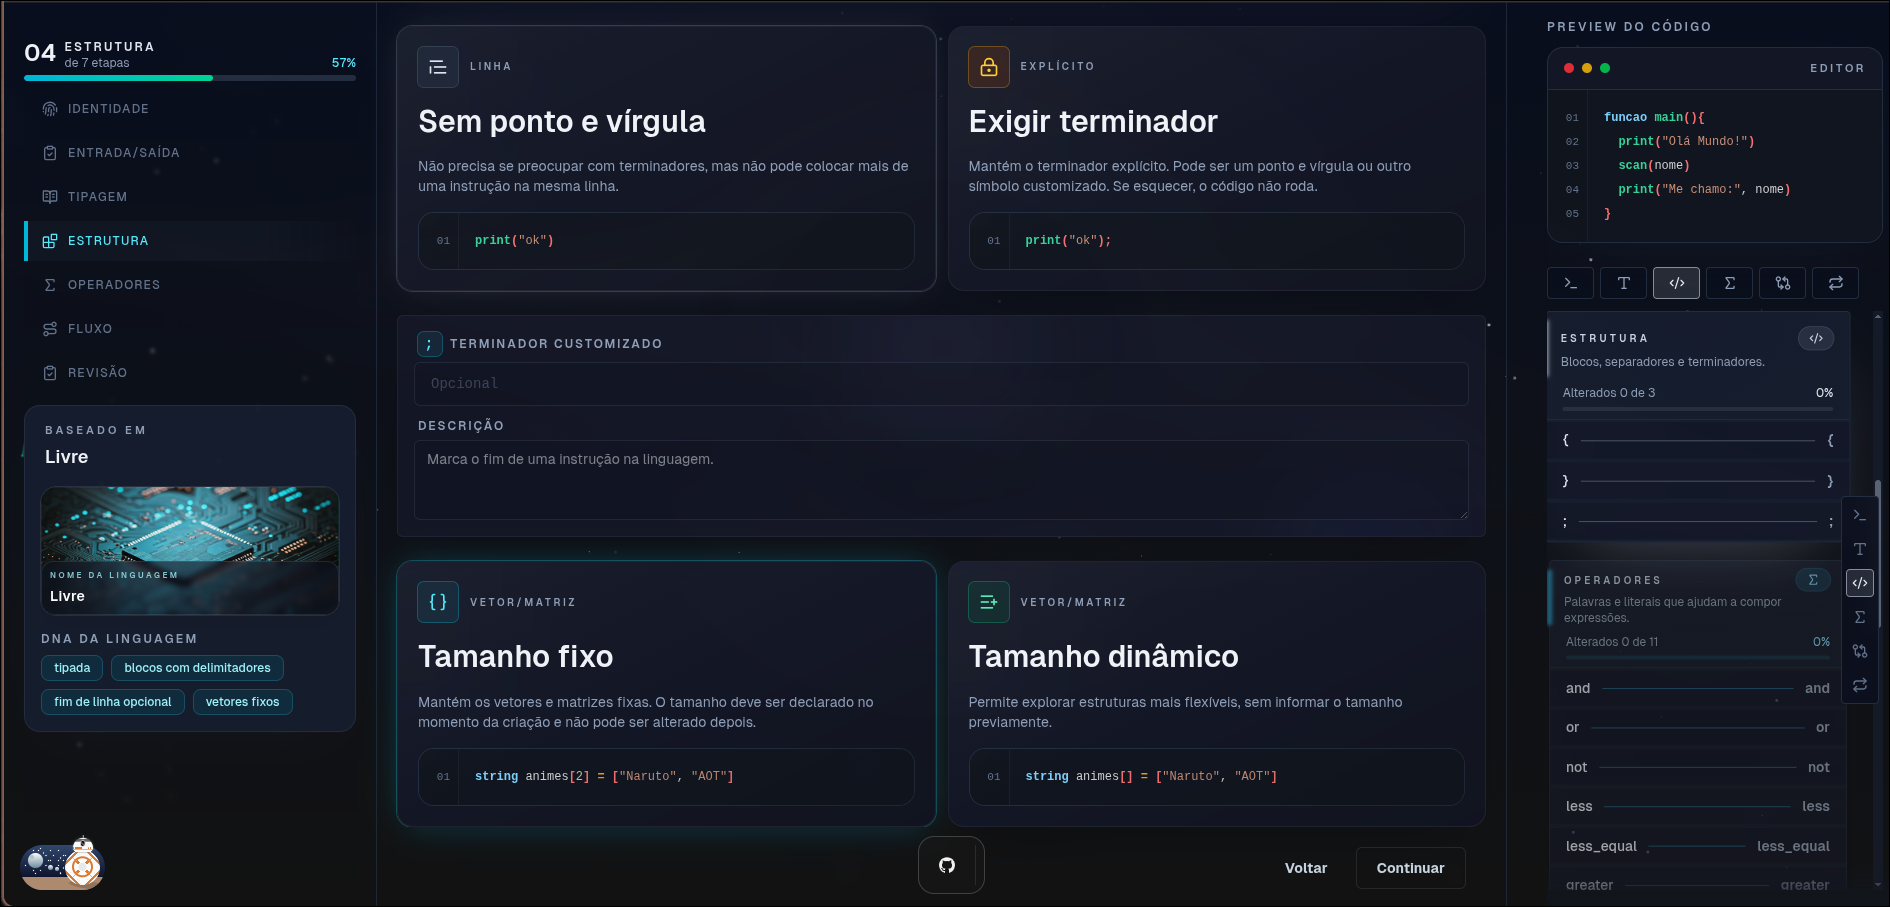
\includegraphics[width=\textwidth]{Etapas/etapa4_2.png}
        \caption{Etapa 4.2: operadores relacionais em forma de palavra.}
        \label{fig:etapa4-2}
    \end{subfigure}
    \caption{Etapa 4 do assistente, dedicada à substituição de operadores por palavras.}
    \label{fig:etapas-4}
    \legend{Fonte: elaborado pelo autor.}
\end{figure}

\FloatBarrier

A quinta etapa, apresentada na Figura~\ref{fig:etapa5}, é responsável pela configuração dos literais booleanos, oferecendo ao usuário a oportunidade de adotar termos como \texttt{verdadeiro} e \texttt{falso} em substituição aos canônicos \texttt{true} e \texttt{false}. A finalização do assistente ocorre na etapa seis, na qual o usuário define os delimitadores de bloco (chaves, palavras-chave ou indentação) e o terminador de instrução, conforme ilustrado pela Figura~\ref{fig:etapas-6}, que reúne as três variações dessa etapa: configuração dos delimitadores, do terminador e da pré-visualização consolidada da linguagem personalizada.

\begin{figure}[H]
    \centering
    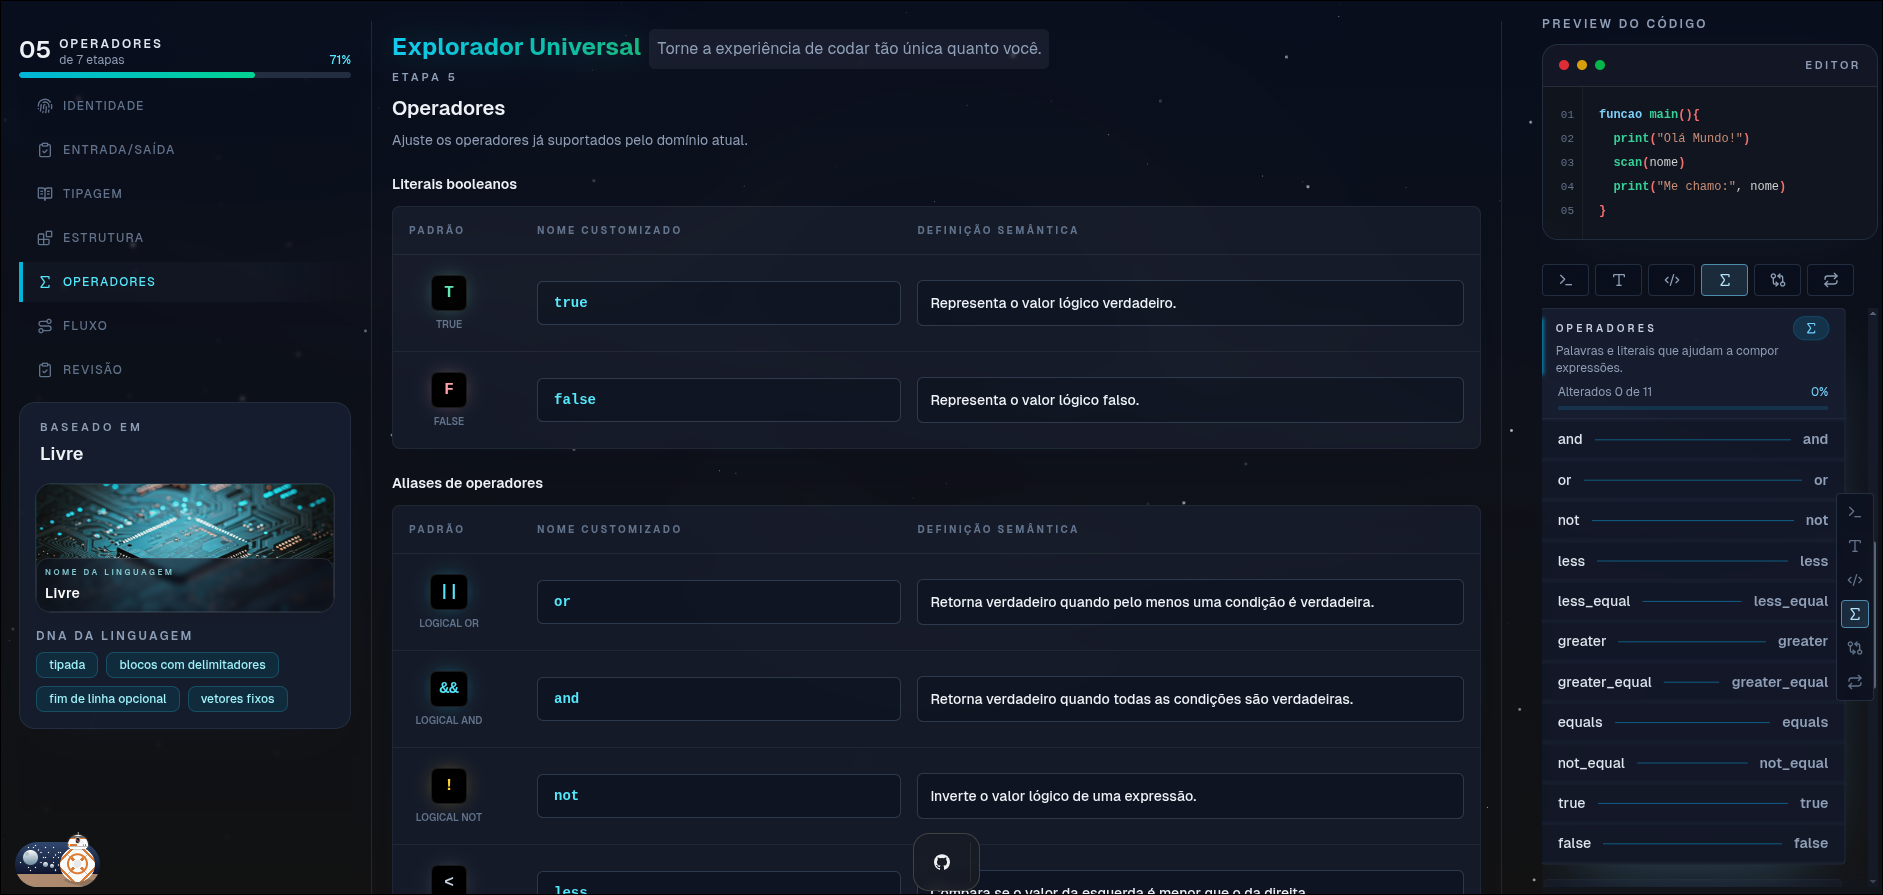
\includegraphics[height=7cm,keepaspectratio]{Etapas/etapa5_1.png}
    \caption{Etapa 5: personalização dos literais booleanos.}
    \label{fig:etapa5}
    \legend{Fonte: elaborado pelo autor.}
\end{figure}

\begin{figure}[p]
    \centering
    \begin{subfigure}{0.9\textwidth}
        \centering
        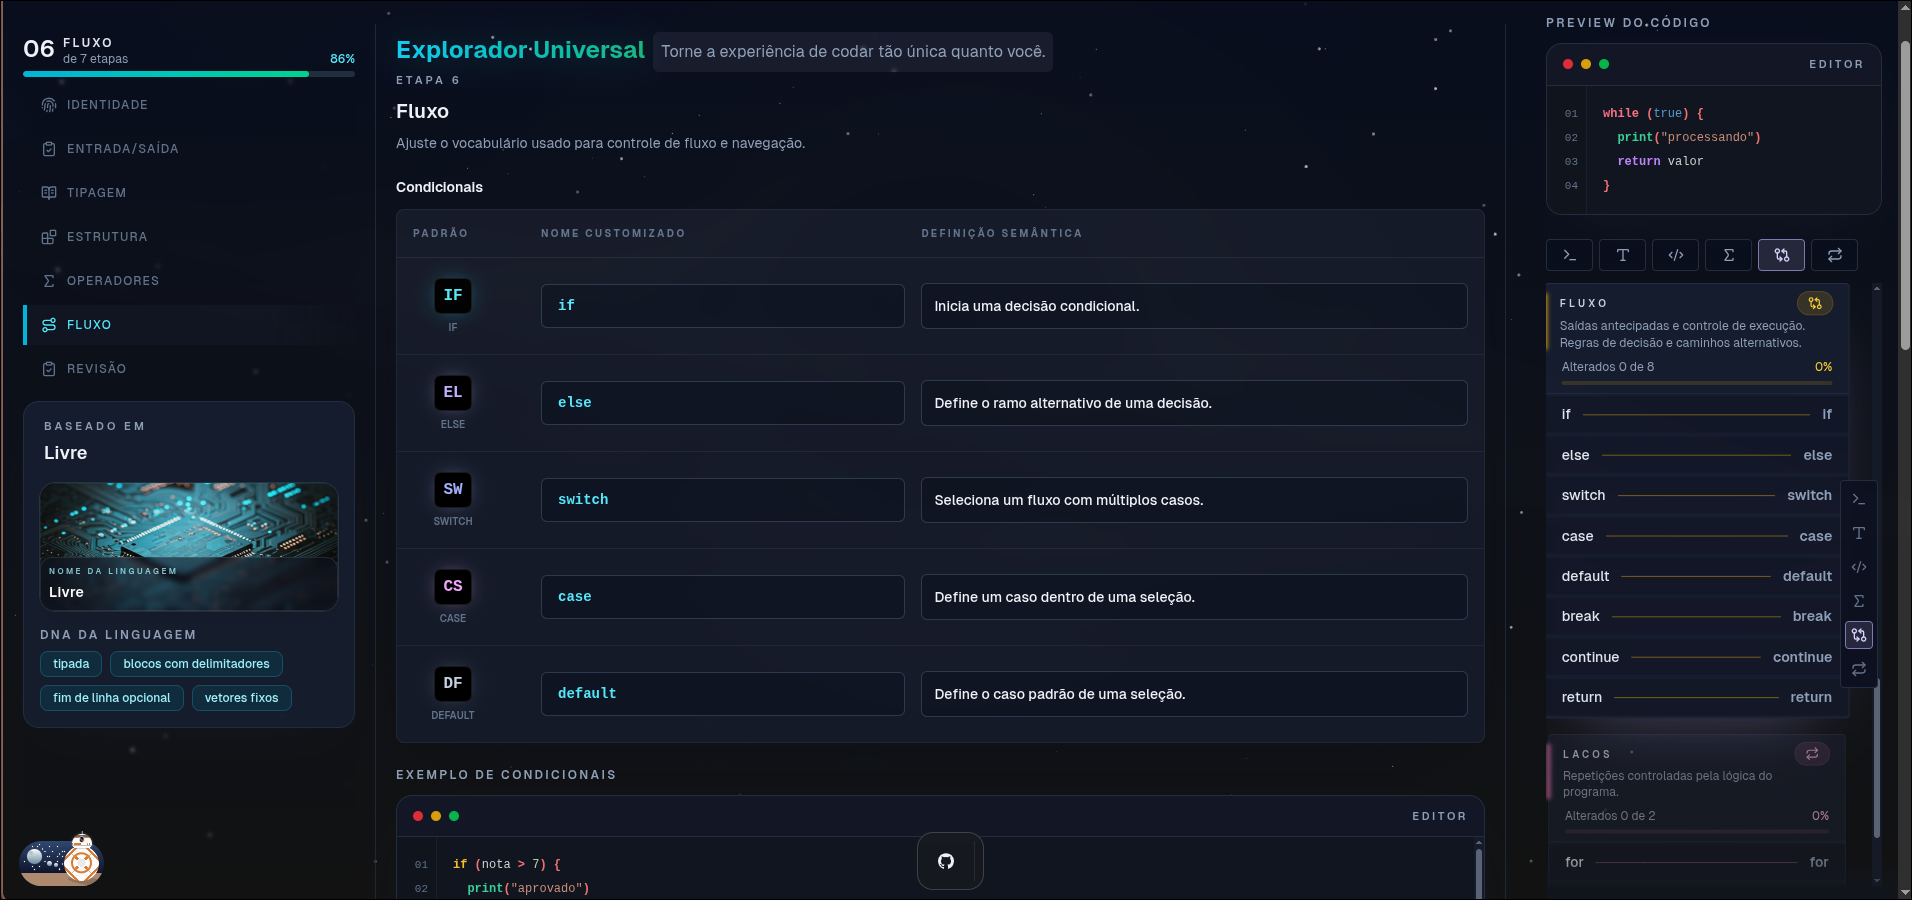
\includegraphics[width=\textwidth]{Etapas/etapa6_1.png}
        \caption{Delimitadores de bloco.}
        \label{fig:etapa6-1}
    \end{subfigure}

    \vspace{0.8em}

    \begin{subfigure}{0.9\textwidth}
        \centering
        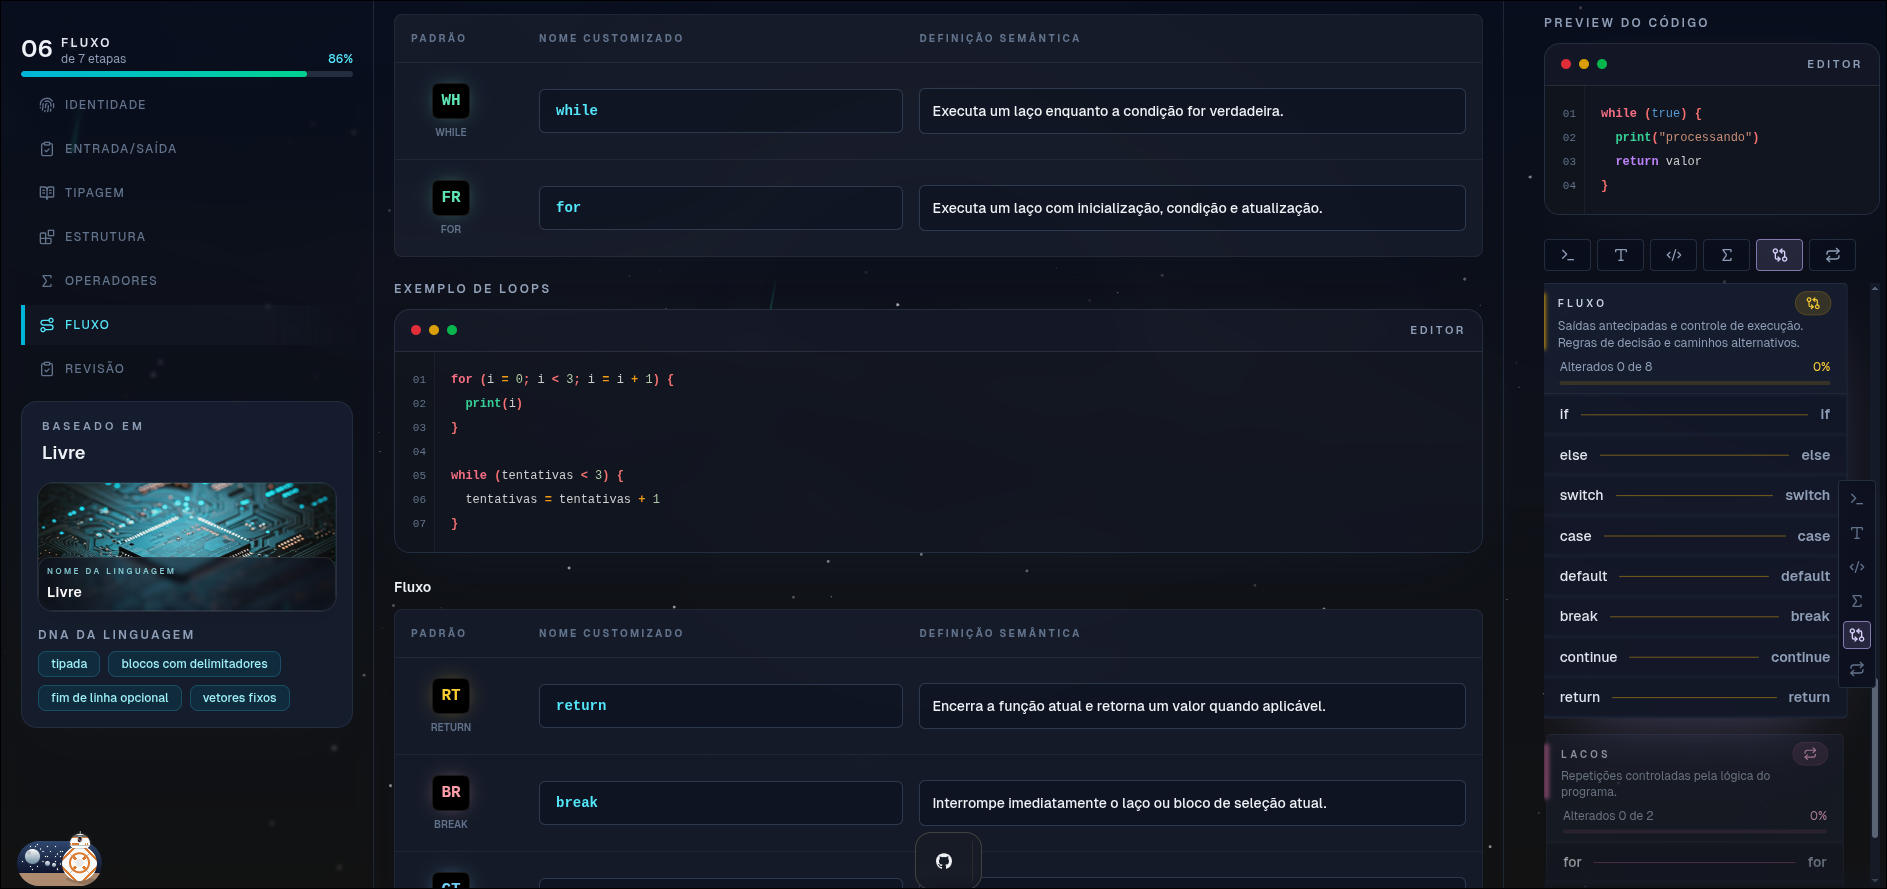
\includegraphics[width=\textwidth]{Etapas/etapa6_2.png}
        \caption{Terminador de instrução.}
        \label{fig:etapa6-2}
    \end{subfigure}

\end{figure}

\begin{figure}[p]\ContinuedFloat
    \centering

    \begin{subfigure}{0.9\textwidth}
        \centering
        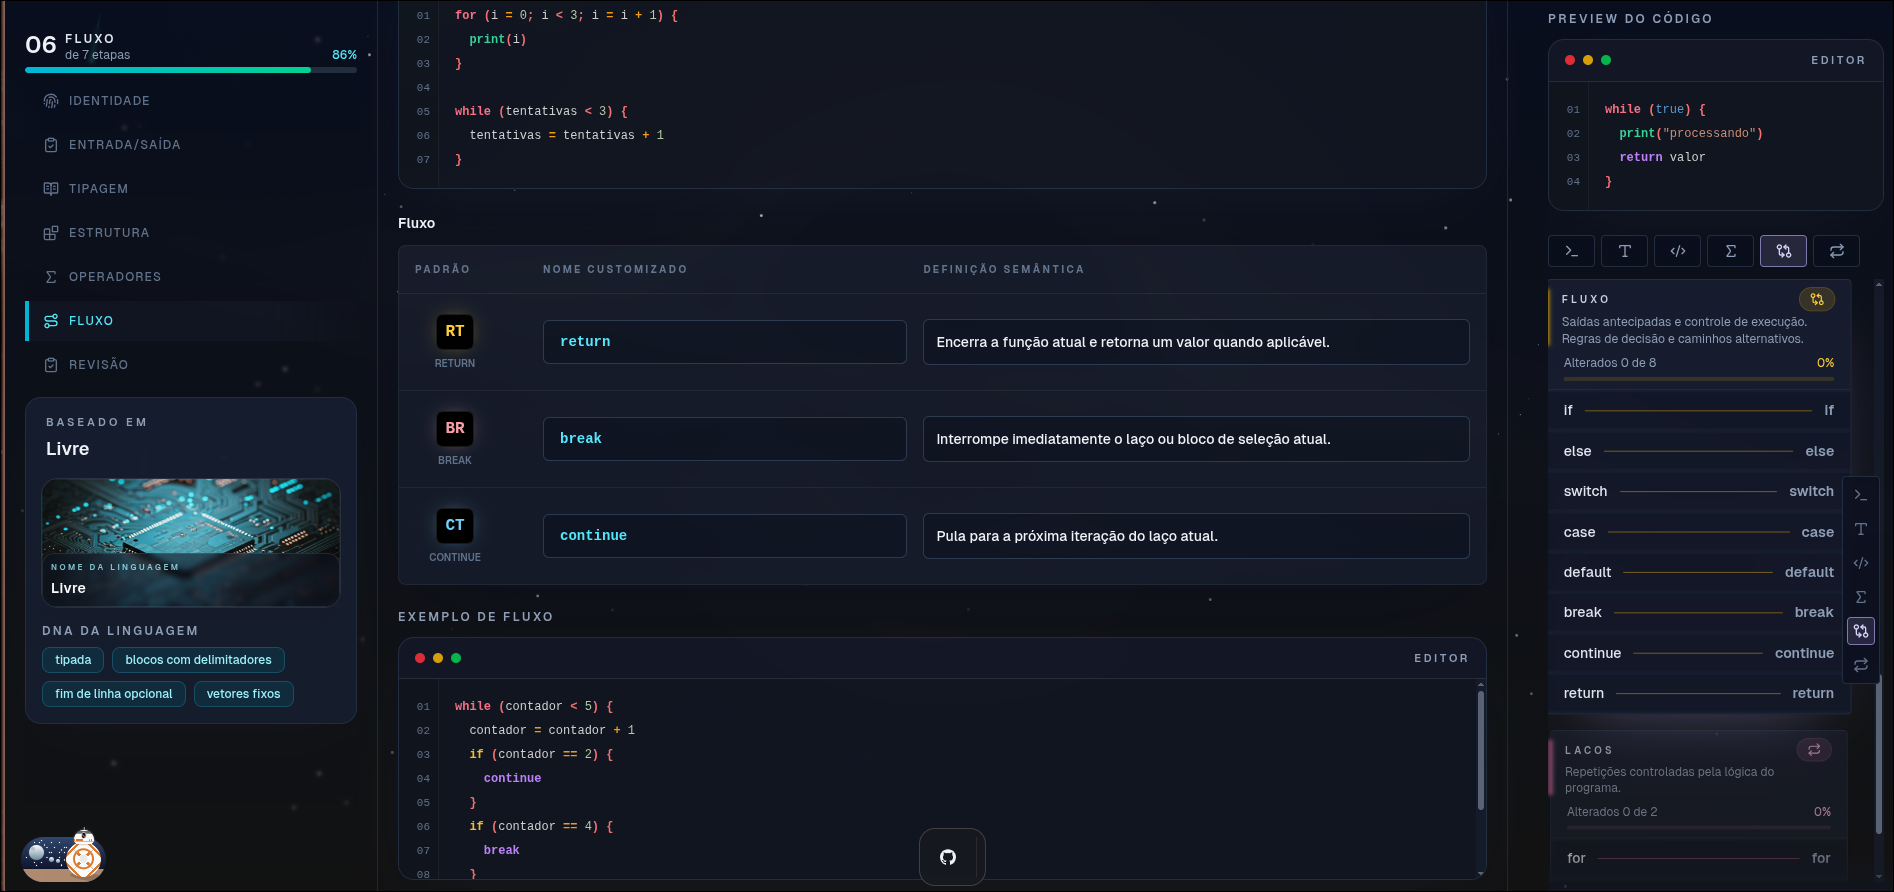
\includegraphics[width=\textwidth]{Etapas/etapa6_3.png}
        \caption{Pré-visualização final.}
        \label{fig:etapa6-3}
    \end{subfigure}
    \caption{Etapa 6 do assistente, dedicada aos delimitadores, ao terminador de instrução e à pré-visualização da linguagem personalizada.}
    \label{fig:etapas-6}
    \legend{Fonte: elaborado pelo autor.}
\end{figure}

\FloatBarrier

O conjunto de telas apresentado consolida, sob o ponto de vista visual, as decisões arquiteturais e de modelagem discutidas ao longo deste capítulo. A organização das informações, a coerência entre os perfis de aluno e professor, a granularidade do assistente de personalização e o cuidado com a paridade entre os temas claro e escuro evidenciam o esforço consciente em alinhar a experiência de uso da plataforma aos princípios de UX e de design inclusivo discutidos no referencial teórico.

\section{Estratégia de Testes Automatizados}
\label{sec:testes-plataforma}

A validação contínua da plataforma foi sustentada por uma suíte de testes automatizados construída com o \textit{framework} Vitest, complementada por \textit{jsdom} para simulação do ambiente de navegador em testes que envolvem componentes React. A organização dos testes refletiu a topologia interna do projeto: testes unitários acompanham diretamente os módulos correspondentes em diretórios \texttt{\_\_tests\_\_}, enquanto testes de integração foram concentrados em arquivos com sufixos \texttt{.spec.ts} ou \texttt{.spec.tsx} próximos aos componentes que validam.

A adoção do TDD discutido por \citeonline{aniche2012} foi particularmente útil em construções críticas, como o validador de palavras-chave personalizadas, o construtor de \textit{preview} interativo da customização, o adaptador do grafo de gramática e o \textit{pipeline} de validação de submissões. Nesses pontos, pequenas alterações na lógica poderiam comprometer fluxos inteiros da plataforma, e a presença de testes automatizados garantiu a estabilidade do comportamento mesmo diante de refatorações estruturais frequentes. Em conformidade com a pirâmide de testes discutida por \citeonline{martin_clean}, a maior parte da suíte concentra-se no nível unitário, garantindo execuções rápidas e \textit{feedback} imediato, enquanto os testes de integração verificam o comportamento agregado entre componentes, \textit{contexts} e \textit{hooks}.

Os mesmos testes são executados localmente durante o desenvolvimento e também acionados pelo \textit{pipeline} de integração contínua antes da incorporação de qualquer mudança ao ramo principal do repositório, assegurando que as características essenciais da plataforma, como a consistência da customização ativa entre recarregamentos, a sincronização correta entre o editor e o sistema de arquivos virtual, a fidelidade do \textit{feedback} de erros ao usuário e a correção dos resultados das submissões, sejam preservadas ao longo de toda a evolução incremental do projeto.



\chapter{CONSIDERAÇÕES FINAIS} \label{cap:consideracoes}
Este capítulo retoma os objetivos, os resultados técnicos apresentados nesta revisão para o TCC~II e as limitações que ainda condicionam a avaliação da plataforma.

\section{Retomada dos Objetivos}

O objetivo geral foi projetar, implementar e integrar uma IDE web ao núcleo de tradução e execução configurável. Os fluxos apresentados no Capítulo~\ref{cap:metodologia} documentam o assistente de personalização, a edição de código, a execução e depuração, a gestão de linguagens e os recursos educacionais de turmas e exercícios.

A especificação dos elementos configuráveis está consolidada na Tabela~\ref{tab:elementos-configuraveis} e na descrição das variantes de análise. A implementação do assistente e dos recursos de edição e execução é apresentada por trechos de código e capturas de tela. A integração utiliza o pacote \texttt{compiler} no navegador e, para a validação de submissões, no servidor Next.js, conforme a Figura~\ref{fig:arquitetura-plataforma}.

A disponibilização técnica permite executar os fluxos locais no navegador. Nesta revisão, 120 testes selecionados pela configuração de integração da IDE foram aprovados, e a Seção~\ref{sec:acessibilidade-responsividade} registra uma verificação delimitada da interface. Os resultados não permitem considerar concluídos os requisitos de acessibilidade, contraste e internacionalização integral, nem demonstram a disponibilidade de uma implantação pública específica.

O objetivo de propor um protocolo de avaliação foi atendido pela Seção~\ref{sec:protocolo-avaliacao}, que relaciona tarefas, decisões de interface, medidas e instrumentos de coleta. A proposta ainda requer definição da amostra, revisão dos instrumentos e encaminhamento institucional antes de sua aplicação. Não se trata de uma avaliação já realizada.

\section{Limitações}

A principal limitação é a ausência de dados de estudantes. O artefato permite investigar a personalização da linguagem, mas ainda não responde empiricamente em que medida essa personalização reduz a barreira sintática. Não se apresentam resultados de aprendizagem, redução de carga cognitiva ou aumento de engajamento.

A verificação de acessibilidade abrange um recorte do assistente, em um navegador, com testes automatizados e uma transição por teclado. Os problemas encontrados exigem ajustes na aplicação; faltam a inspeção dos processos completos e a verificação com tecnologias assistivas. O uso de bibliotecas de componentes não sustenta uma presunção de conformidade.

A configuração de testes utilizada não inclui todos os arquivos existentes, e o fluxo de implantação versionado não demonstra execução automática do Vitest. Também não foram conduzidas medições de desempenho nem auditoria de segurança. A configuração do token em \textit{cookie} acessível por JavaScript e a ausência de isolamento de processo na avaliação de programas são aspectos que exigem análise técnica específica antes de ampliar o cenário de uso.

A linguagem oferece construções imperativas e variantes de tipagem e de arranjos implementadas no núcleo. Não permite acrescentar gramáticas arbitrárias, orientação a objetos ou modularização de um programa em múltiplos arquivos de código-fonte. O sistema de arquivos virtual da IDE organiza documentos, sem representar, por si só, um mecanismo de módulos da linguagem.

\section{Encaminhamentos}

Os próximos passos técnicos são corrigir os problemas de acessibilidade documentados, verificar os fluxos completos de teclado e leitor de tela, revisar os textos ainda não internacionalizados e integrar a execução dos testes ao processo de incorporação de mudanças. As capturas históricas da implementação devem ser atualizadas conforme a interface se estabilize para a apresentação final.

No plano metodológico, a continuidade consiste em revisar e aplicar o protocolo proposto, depois de definir participantes, instrumentos e procedimentos institucionais. Só então será possível discutir resultados de uso e investigar a contribuição pedagógica da personalização. O compartilhamento de linguagens, já implementado no catálogo comunitário e na vinculação a exercícios e listas, poderá ser estudado como recurso didático em turmas; a exportação para uso fora da plataforma permanece outro possível desdobramento.


%% -----------Elementos  Pós-Textuais --------------

\postextual

\bibliography{referencias.bib}

\appendix

\chapter[APÊNDICE A -- PLANO DE TRABALHO: DIVISÃO DE RESPONSABILIDADES]{{\centering APÊNDICE A \textendash{} PLANO DE TRABALHO: DIVISÃO DE RESPONSABILIDADES}}  \label{ap:plano}

Este apêndice detalha a divisão de responsabilidades entre os dois autores, conforme a pré-proposta aprovada e o plano de trabalho entregue à Coordenação do Curso de Engenharia de Computação do Centro Federal de Educação Tecnológica de Minas Gerais, Unidade Leopoldina.

\section{Atividades Desenvolvidas em Regime Colaborativo}

As atividades listadas a seguir foram conduzidas de forma conjunta por Igor Lamoia Queiroz e Victor de Souza Vilela da Silva, com participação efetiva de ambos os integrantes nas etapas de especificação, implementação, integração e revisão:

\begin{itemize}
    \item Revisão bibliográfica sobre interpretadores, compiladores e ferramentas educacionais relacionadas;
    \item Definição dos requisitos funcionais e não funcionais e da arquitetura geral do sistema;
    \item Participação na implementação e validação do núcleo do compilador, incluindo análise léxica, análise sintática, geração e execução de código intermediário;
    \item Especificação dos mecanismos de injeção dinâmica de regras gramaticais e integração desses mecanismos à experiência de personalização da IDE;
    \item Integração do núcleo do interpretador com a plataforma web e definição dos contratos de comunicação entre os módulos;
    \item Revisão mútua de código e tomada de decisões arquiteturais nas etapas de refatoração e evolução do sistema.
\end{itemize}

\section{Eixos de Aprofundamento Individual}

A partir da base técnica construída em conjunto, cada autor concentrou seu aprofundamento acadêmico em eixos específicos, conforme estabelecido na pré-proposta.

\subsection{Igor Lamoia Queiroz (este documento)}

\begin{itemize}
    \item Detalhamento da arquitetura da aplicação web (Next.js, Pages Router) e da integração com o Monaco Editor para edição de código com realce de sintaxe configurável;
    \item Documentação da customização dinâmica de \textit{tokens} e sintaxe por meio do assistente de personalização da linguagem (\textit{wizard}), incluindo o modelo de etapas, a lógica de validação preventiva e o mecanismo de pré-visualização em tempo real;
    \item Análise da experiência de uso da plataforma, dos contextos React que governam o estado da aplicação e das mediações pedagógicas oferecidas pela interface ao estudante iniciante;
    \item Descrição da execução das análises léxica e sintática com o código produzido na IDE e da apresentação do código intermediário no terminal integrado;
    \item Estudos de caso centrados na usabilidade, no engajamento dos estudantes e no \textit{feedback} coletado em ambiente educacional.
\end{itemize}

\subsection{Victor de Souza Vilela da Silva (documento complementar)}

\begin{itemize}
    \item Detalhamento das fases de análise léxica e do sistema de varredura por escâneres especializados (\textit{factory pattern});
    \item Descrição aprofundada da análise sintática por descida recursiva e da correspondência entre as produções do analisador e a gramática formal da linguagem Java-{}-;
    \item Documentação da geração de código de três endereços: instrução a instrução, tabela de temporários e tabela de rótulos;
    \item Análise do funcionamento do interpretador, da tabela de símbolos e do despacho das chamadas de sistema de entrada e saída;
    \item Desenvolvimento do \textit{back-end} da plataforma em FastAPI, incluindo a modelagem das entidades de domínio, a implementação das rotas REST, a persistência com SQLAlchemy assíncrono e o suporte a autenticação, turmas, exercícios, listas e submissões;
    \item Estudos de caso centrados na validade técnica do núcleo de tradução e no comportamento do interpretador frente a programas de teste elaborados para cobrir as construções da linguagem.
\end{itemize}


%%% ---
\end{document}
